従来手法となる遅延評価法,本稿で提案したLE-Q,LE-QD,ALE-Qの性能を比較する評価実験を行った.
各実験において,
\begin{enumerate}
    \item 実行時間
    \item マッチング判定回数
\end{enumerate}
の比較を行う.また,実験を行う環境として,
Intel(R) Core(TM) i7-6700 CPU @3.40GHz,16GBメモリ,Ubuntu20.04
を用意した.
各実験において以下の設定を用いる.
\begin{itemize}
    \item スライディングウィンドウの大きさ 100
    \item シミュレートする時刻 1から1000
    \item テキスト類似度の閾値$\epsilon_{doc}$を0.1
    \item ユーザ間類似度の閾値$\epsilon_u$を0,10,20,30,40,50,60,70,80,90,100と変化させた.
\end{itemize}

\section{人工データセット}
人工データセットを以下のルールに則って生成した.全ユーザは3単語で構成されるテキストを1000個ずつ持つ.単語集合$\Phi_q,\Phi_{nq}$を用意し,
\begin{itemize}
    \item $\Phi_q \cap \Phi_{nq} = \phi$
    \item $|\Phi_q|=1000$
    \item $|\Phi_{nq}|=1000$
\end{itemize}
とする.
\begin{itemize}
    \item クエリユーザのテキストは$\Phi_q$から重複ありでランダムに選んだ単語で構成する.
    \item データベース側にはユーザを100人用意する.
    $i$番目($1\le i \le 100$)のユーザの時刻$t(1\le t\le 1000)$のテキストは,
    \begin{itemize}
        %\item $0.96^{(i-1)}$の確率で$t-100 \le t' < t+100$を満たす$t'$をランダムに決定し,クエリの時刻$t'$のテキストとする.
        \item $p$の確率で$t-100 \le t' < t+100$を満たす$t'$をランダムに決定し,クエリの時刻$t'$のテキストとする.
        %\item $1-0.96^{(i-1)}$の確率で$\Phi_{nq}$から重複を許してランダムに選んだ単語とする.
        \item $1-p$の確率で$\Phi_{nq}$から重複を許してランダムに選んだ単語とする.
    \end{itemize}
\end{itemize}
以上の条件をもとに以下の6つのデータセットを作成する.
\begin{enumerate}
    \item $p=0.1$としたときのデータセット
    \item $p=0.3$としたときのデータセット
    \item $p=0.5$としたときのデータセット
    \item $p=0.7$としたときのデータセット
    \item $p=0.9$としたときのデータセット
    \item $p=0.96^{(i-1)}$としたときのデータセット
    \begin{itemize}
        \item $i$が小さいほどクエリユーザのテキストを選ぶ確率が大きくなるため,$i$が大きいユーザほど,クエリユーザとの類似度の期待値が小さくなる.
    \end{itemize}
\end{enumerate}
これらのデータセットを用いて,各時刻に1つのテキストが到着する環境をシミュレートする.

\section{CoPhIRデータセット}
実データとしてFlickrアーカイブからメタデータを抽出したCoPhIR(Content-based Photo Image Retrieval)\cite{CoPhIR}\cite{2009}データセットを用いる.
このデータセットの各エントリには以下の内容が含まれている.
\begin{itemize}
    \item Flickr Webサイトの対応するエントリへのリンク
    \item 写真画像のサムネイル
    \item 対応するFlickrエントリ内のFlickrユーザ情報を含むXML構造体
    \begin{itemize}
        \item タイトル
        \item 位置
        \item GPS
        \item タグ
        \item コメント
    \end{itemize}
    \item 5つの標準MPEG-7画像特徴を抽出したXML構造体
    \begin{itemize}
        \item Scalable Colour
        \item Colour Structure
        \item Colour Layout
        \item Edge Histogram
        \item Homogeneous Texture
    \end{itemize}
\end{itemize}


CoPhIRデータセットに含まれる写真のメタデータから写真につけられたタグを単語とみなし,写真1枚に対して1つのテキストとし,本実験に適用した.なお,データセットは9108種類のタグと,100人のユーザから構成される.

ユーザごとに持つ写真の数は異なるが,すべて100個以上であるため,スライディングウィンドウの大きさ以上のテキストを持つ.テキストの数が1000に満たないユーザは古い時刻のテキストから順番に複製し,全ユーザが1000個のテキストを持つデータセットとする.


\section{転置インデクスの性能評価}
\label{exp1}
遅延評価法,LE-Q,LE-QDのアルゴリズムを人工データセット,CoPhIRデータセットを利用し,全ユーザの類似性を各時刻すべてにおいて求める実験を行った.
人工データセットにおける実験結果を図\ref{fig:exp1_art}に示す.
結果よりLE-QはLE-QDよりも高速に動作することが分かった.LE-QDはマッチング比較回数をかなり抑えることができたものの,転置インデクスの構築に時間がかかってしまい,結果的にLE-Qよりも多くの実行時間を要することとなったと考えられる.

\begin{figure}[H]
    \centering
    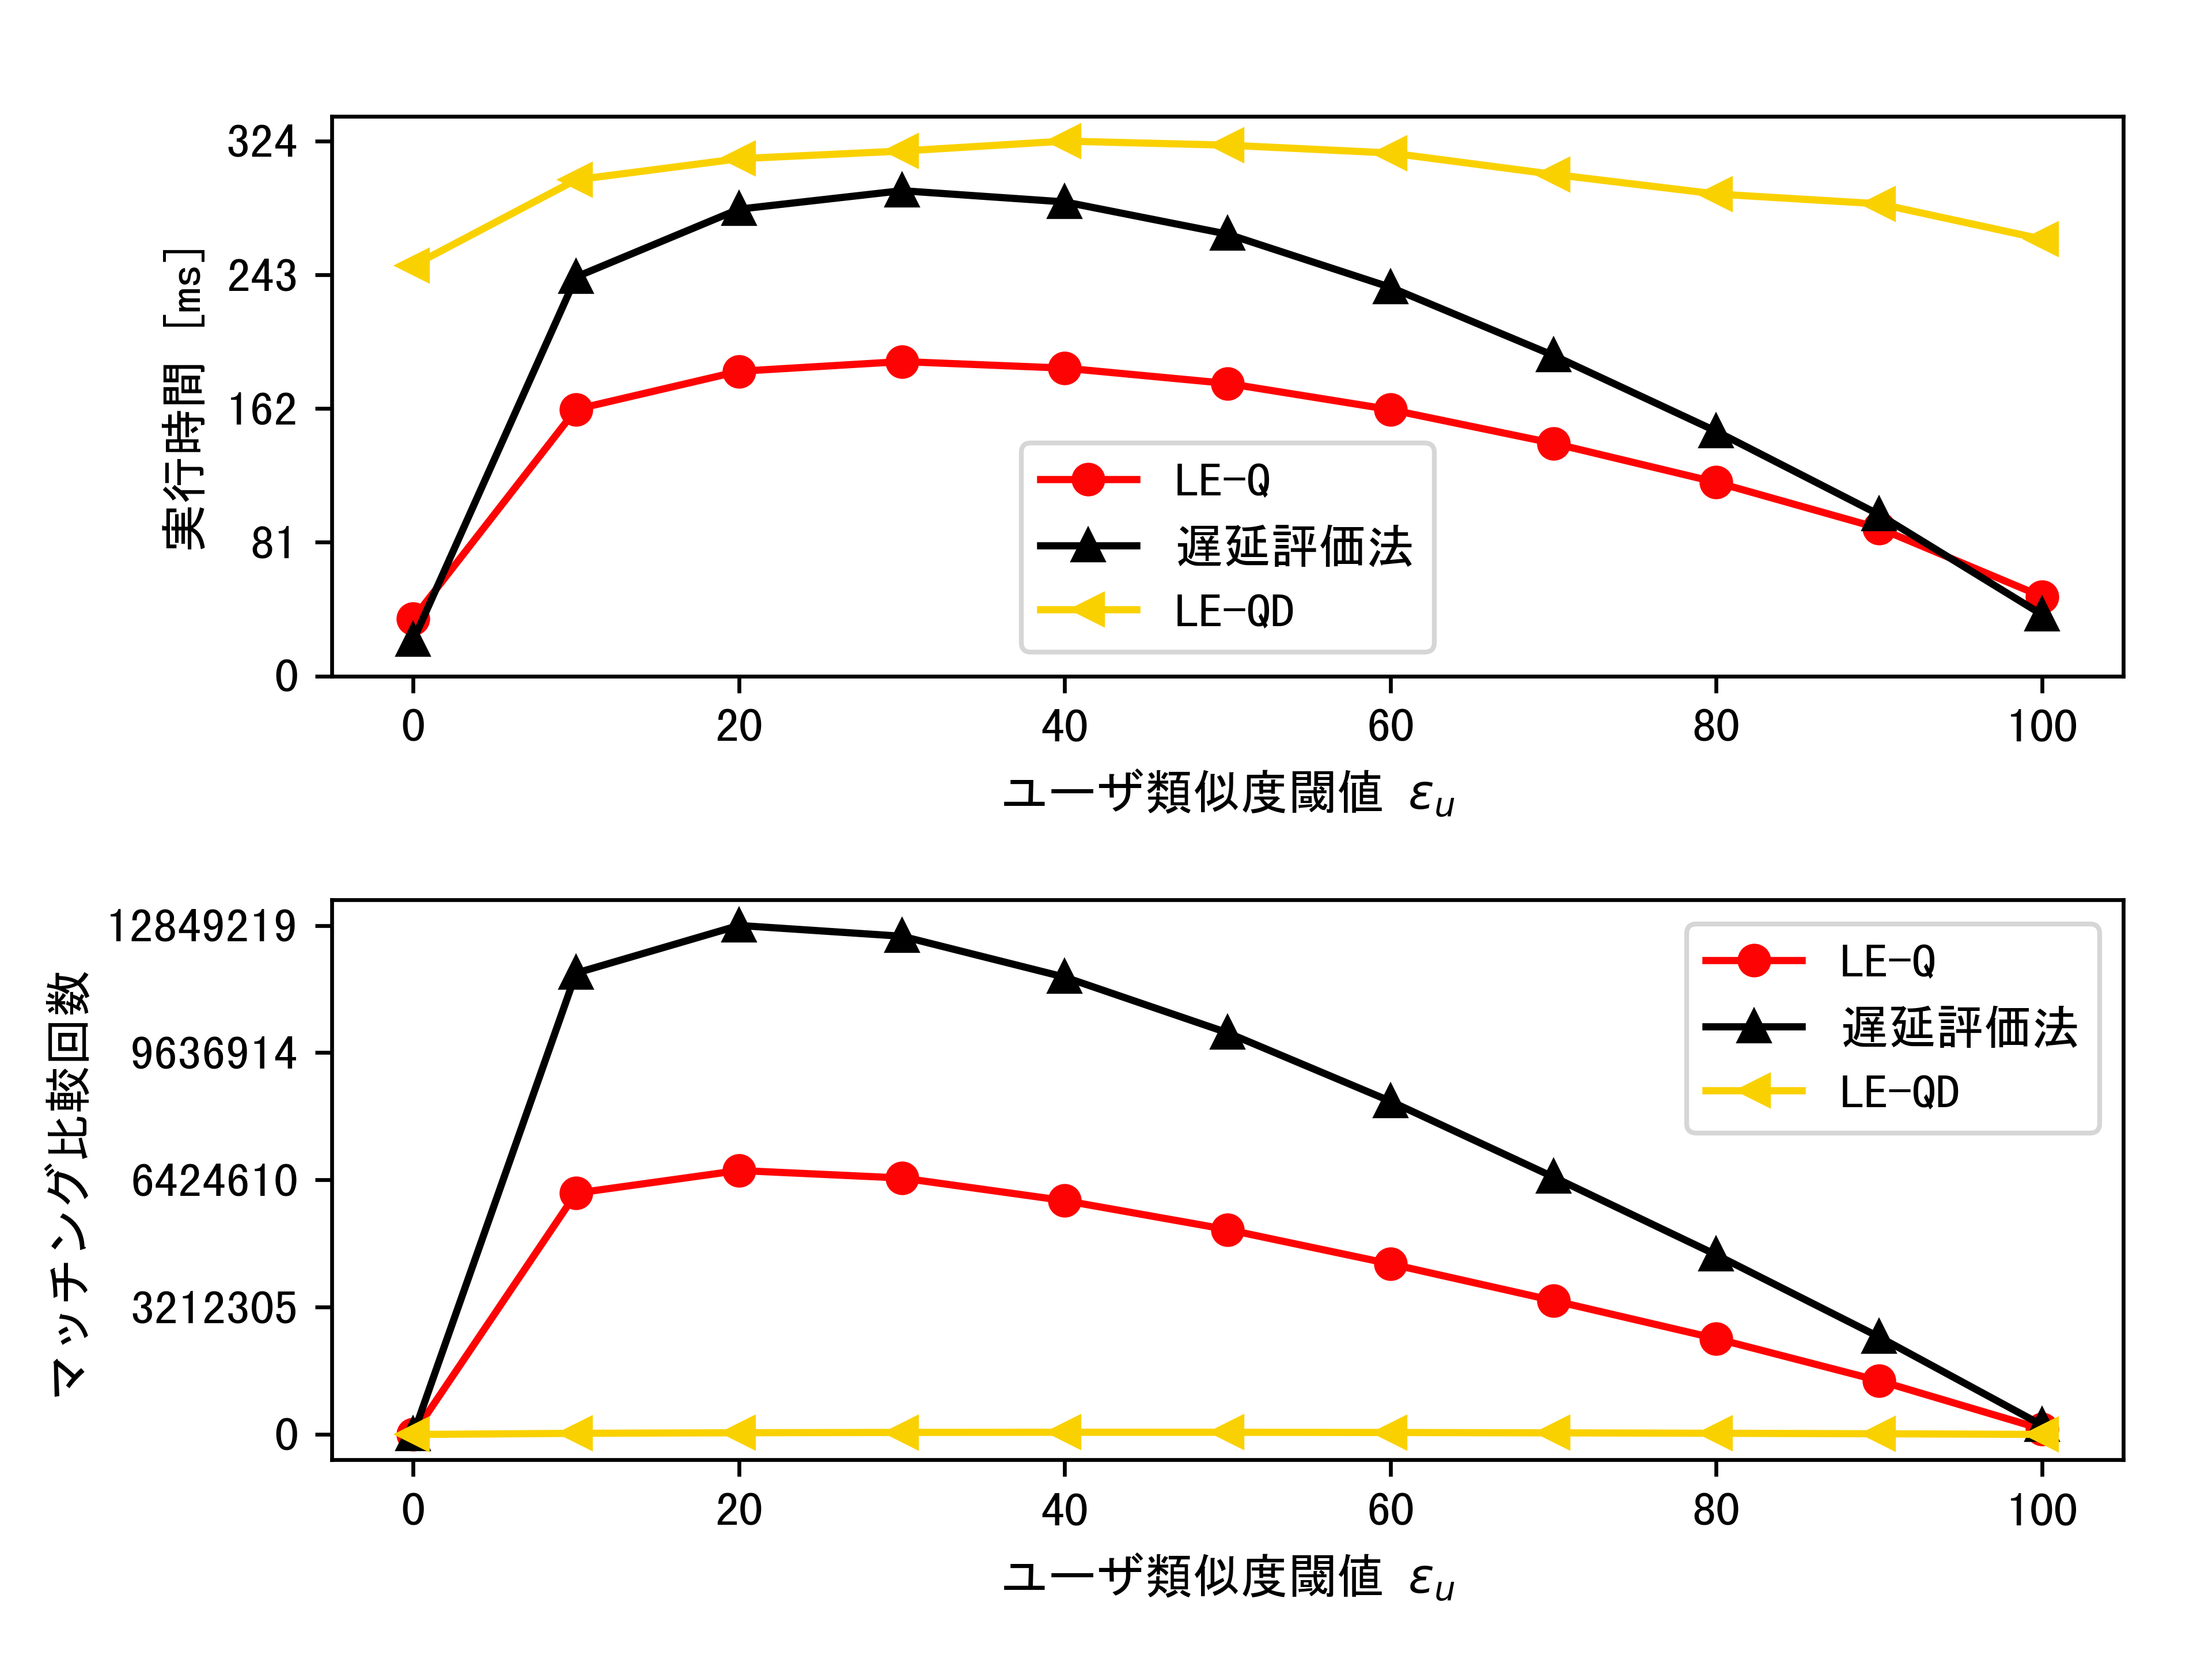
\includegraphics[width=8.3cm]{eimg/exp1.png}
    \caption{性能評価(人工データセット($p=0.96^{(i-1)}$))}
    \label{fig:exp1_art}
\end{figure}
CoPhIRデータセットにおける実験結果を図\ref{fig:exp1_cop}に示した.
%SNSのような現実世界の環境では,クエリユーザに対するデータベースユーザの類似度はほとんどの場合において小さくなると考えられる.そのため,実データのCoPhIRデータセットではLE-Qの方が優位である結果が得られたと考えられる.
図\ref{fig:exp1_art}と同様な結果を示し,LE-QDと遅延評価法よりLE-Qが効率的であると言える.

\begin{figure}[H]
    \centering
    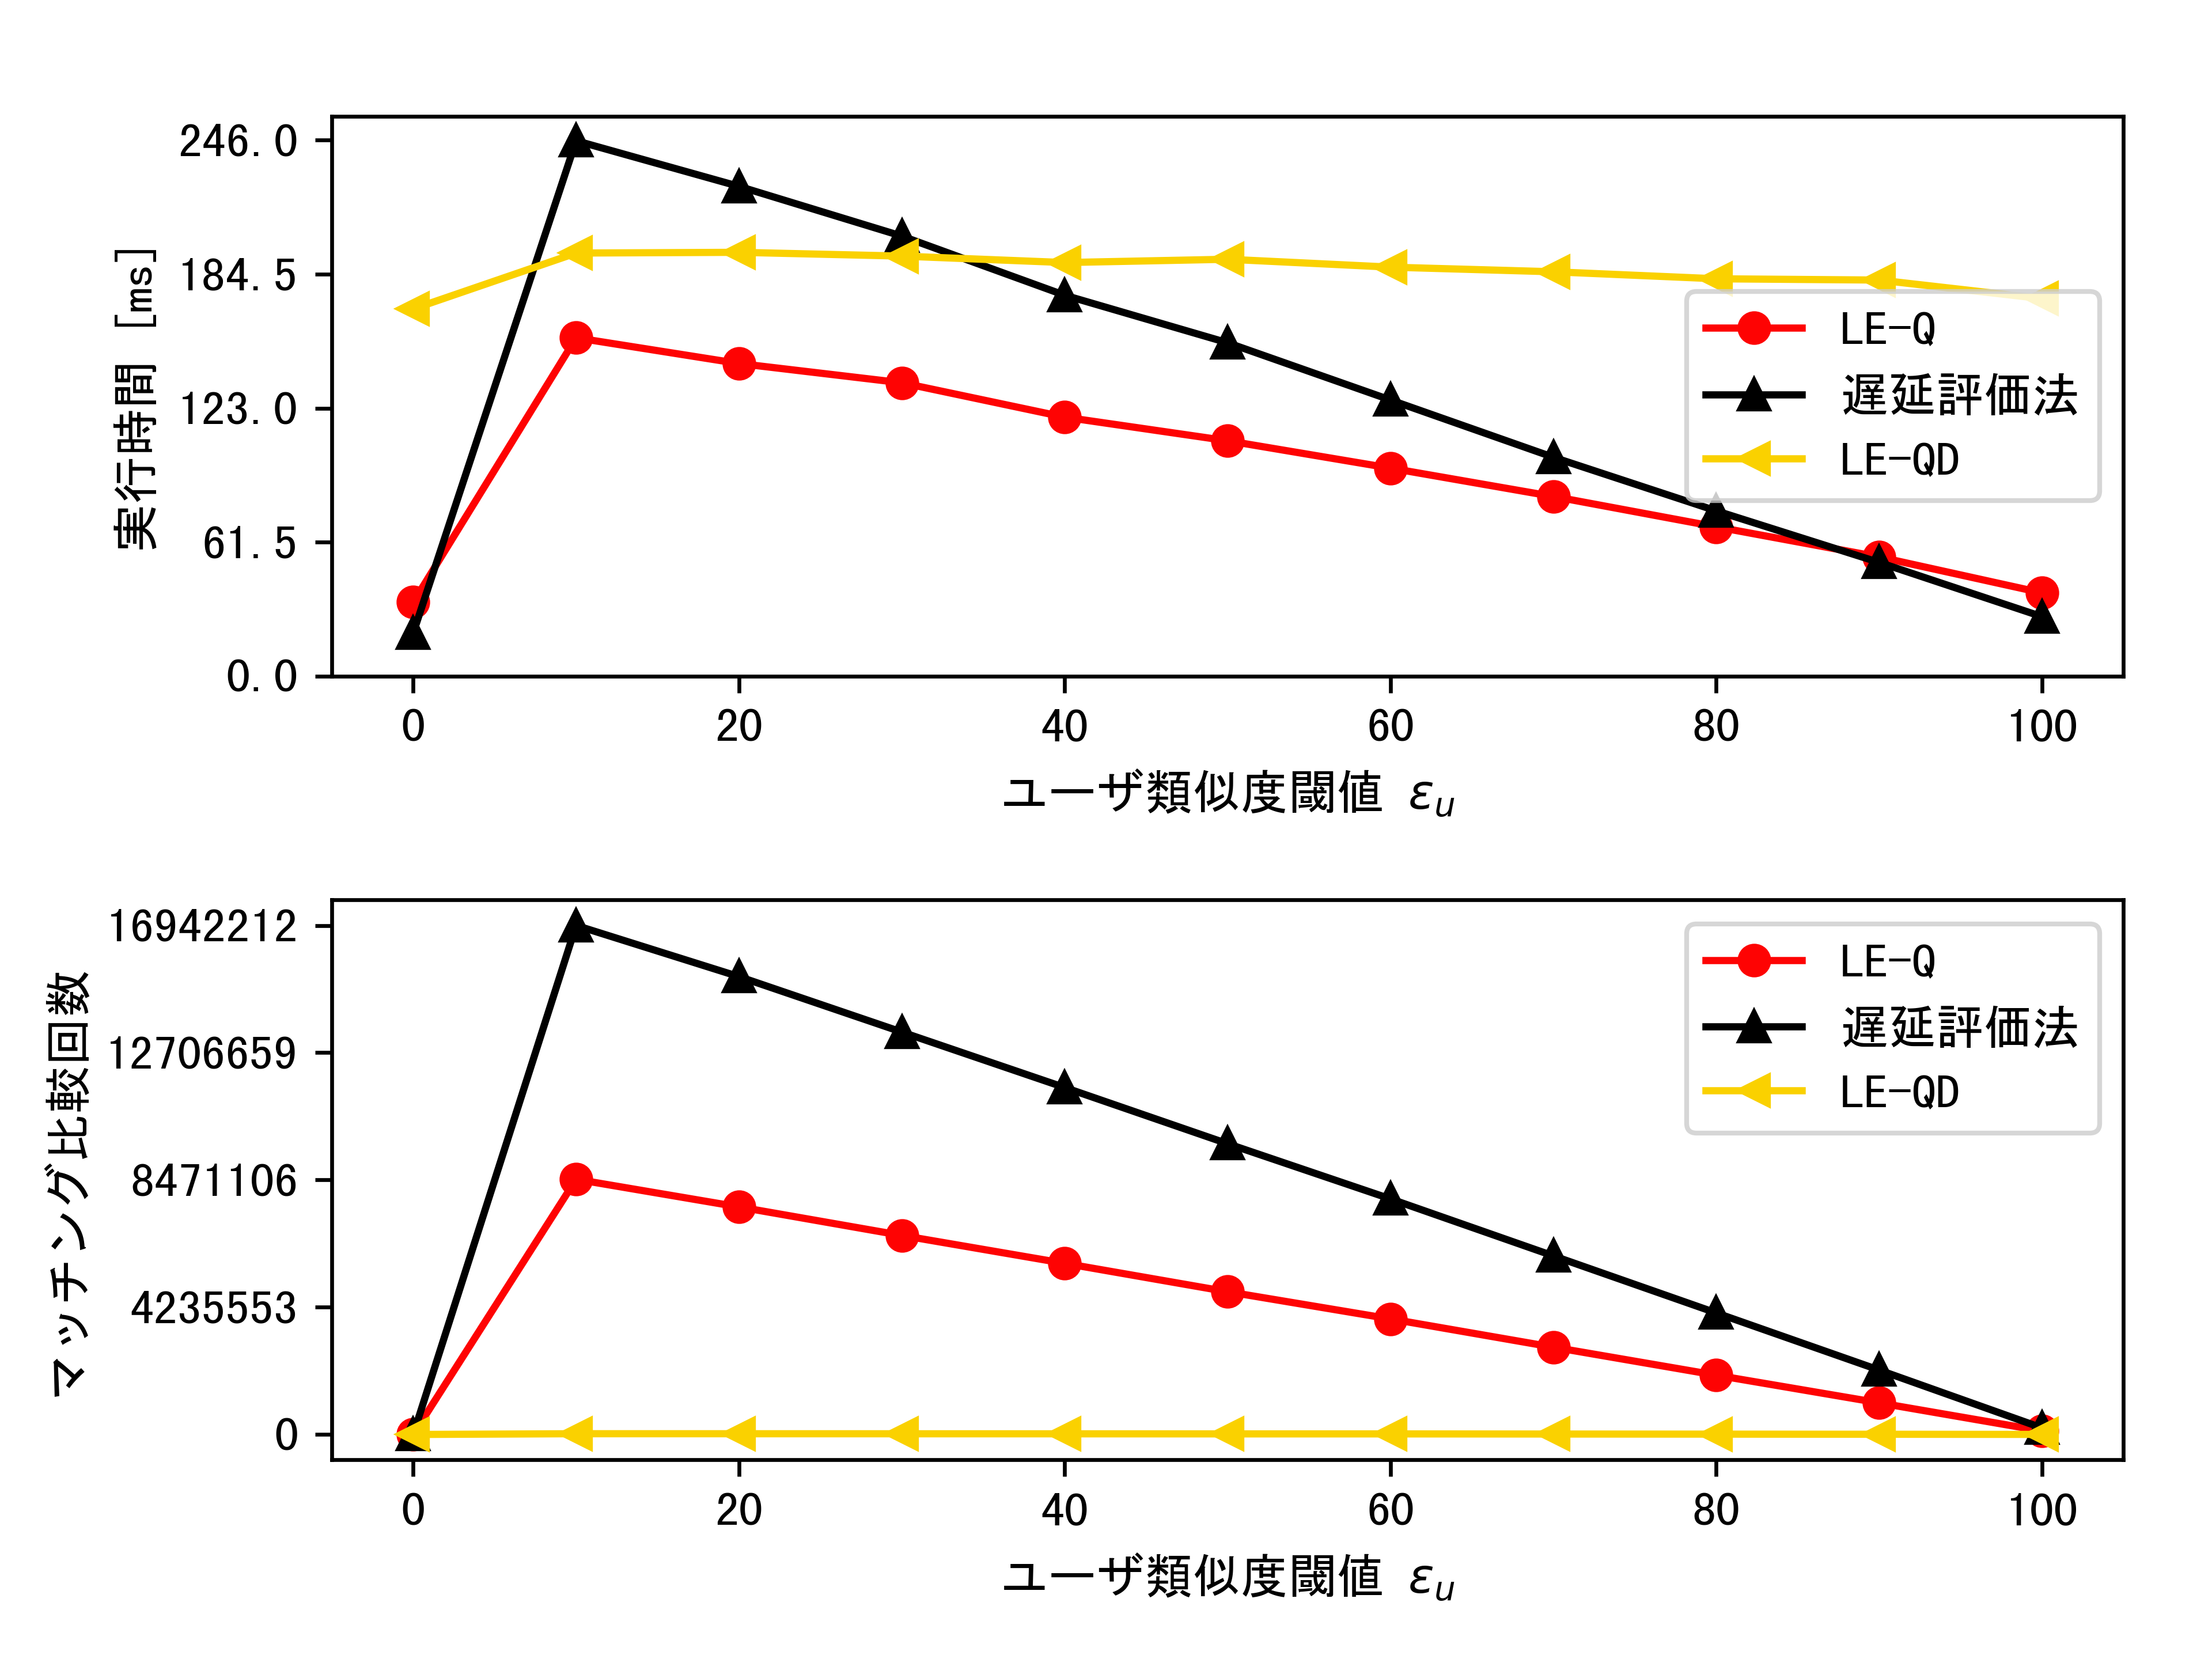
\includegraphics[width=8.3cm]{eimg/exp1_c.png}
    \caption{性能評価(CoPhIRデータセット)}
    \label{fig:exp1_cop}
\end{figure}

人工データセットにおける$p$を固定した場合の実験結果を図\ref{fig:exp1_art_1},図\ref{fig:exp1_art_3},図\ref{fig:exp1_art_5},図\ref{fig:exp1_art_7},図\ref{fig:exp1_art_9}に示した.
%クエリに対するデータベースユーザの類似度が小さい時には遅延評価法よりLE-Qの方が高速であるが,類似度が大きくなるに連れて,LE-Qより遅延評価法の方が高速に動作するような結果になった.
$p$の値によらず,LE-Qが最も効率的に動作していることがわかる.

\begin{figure}[H]
    \centering
    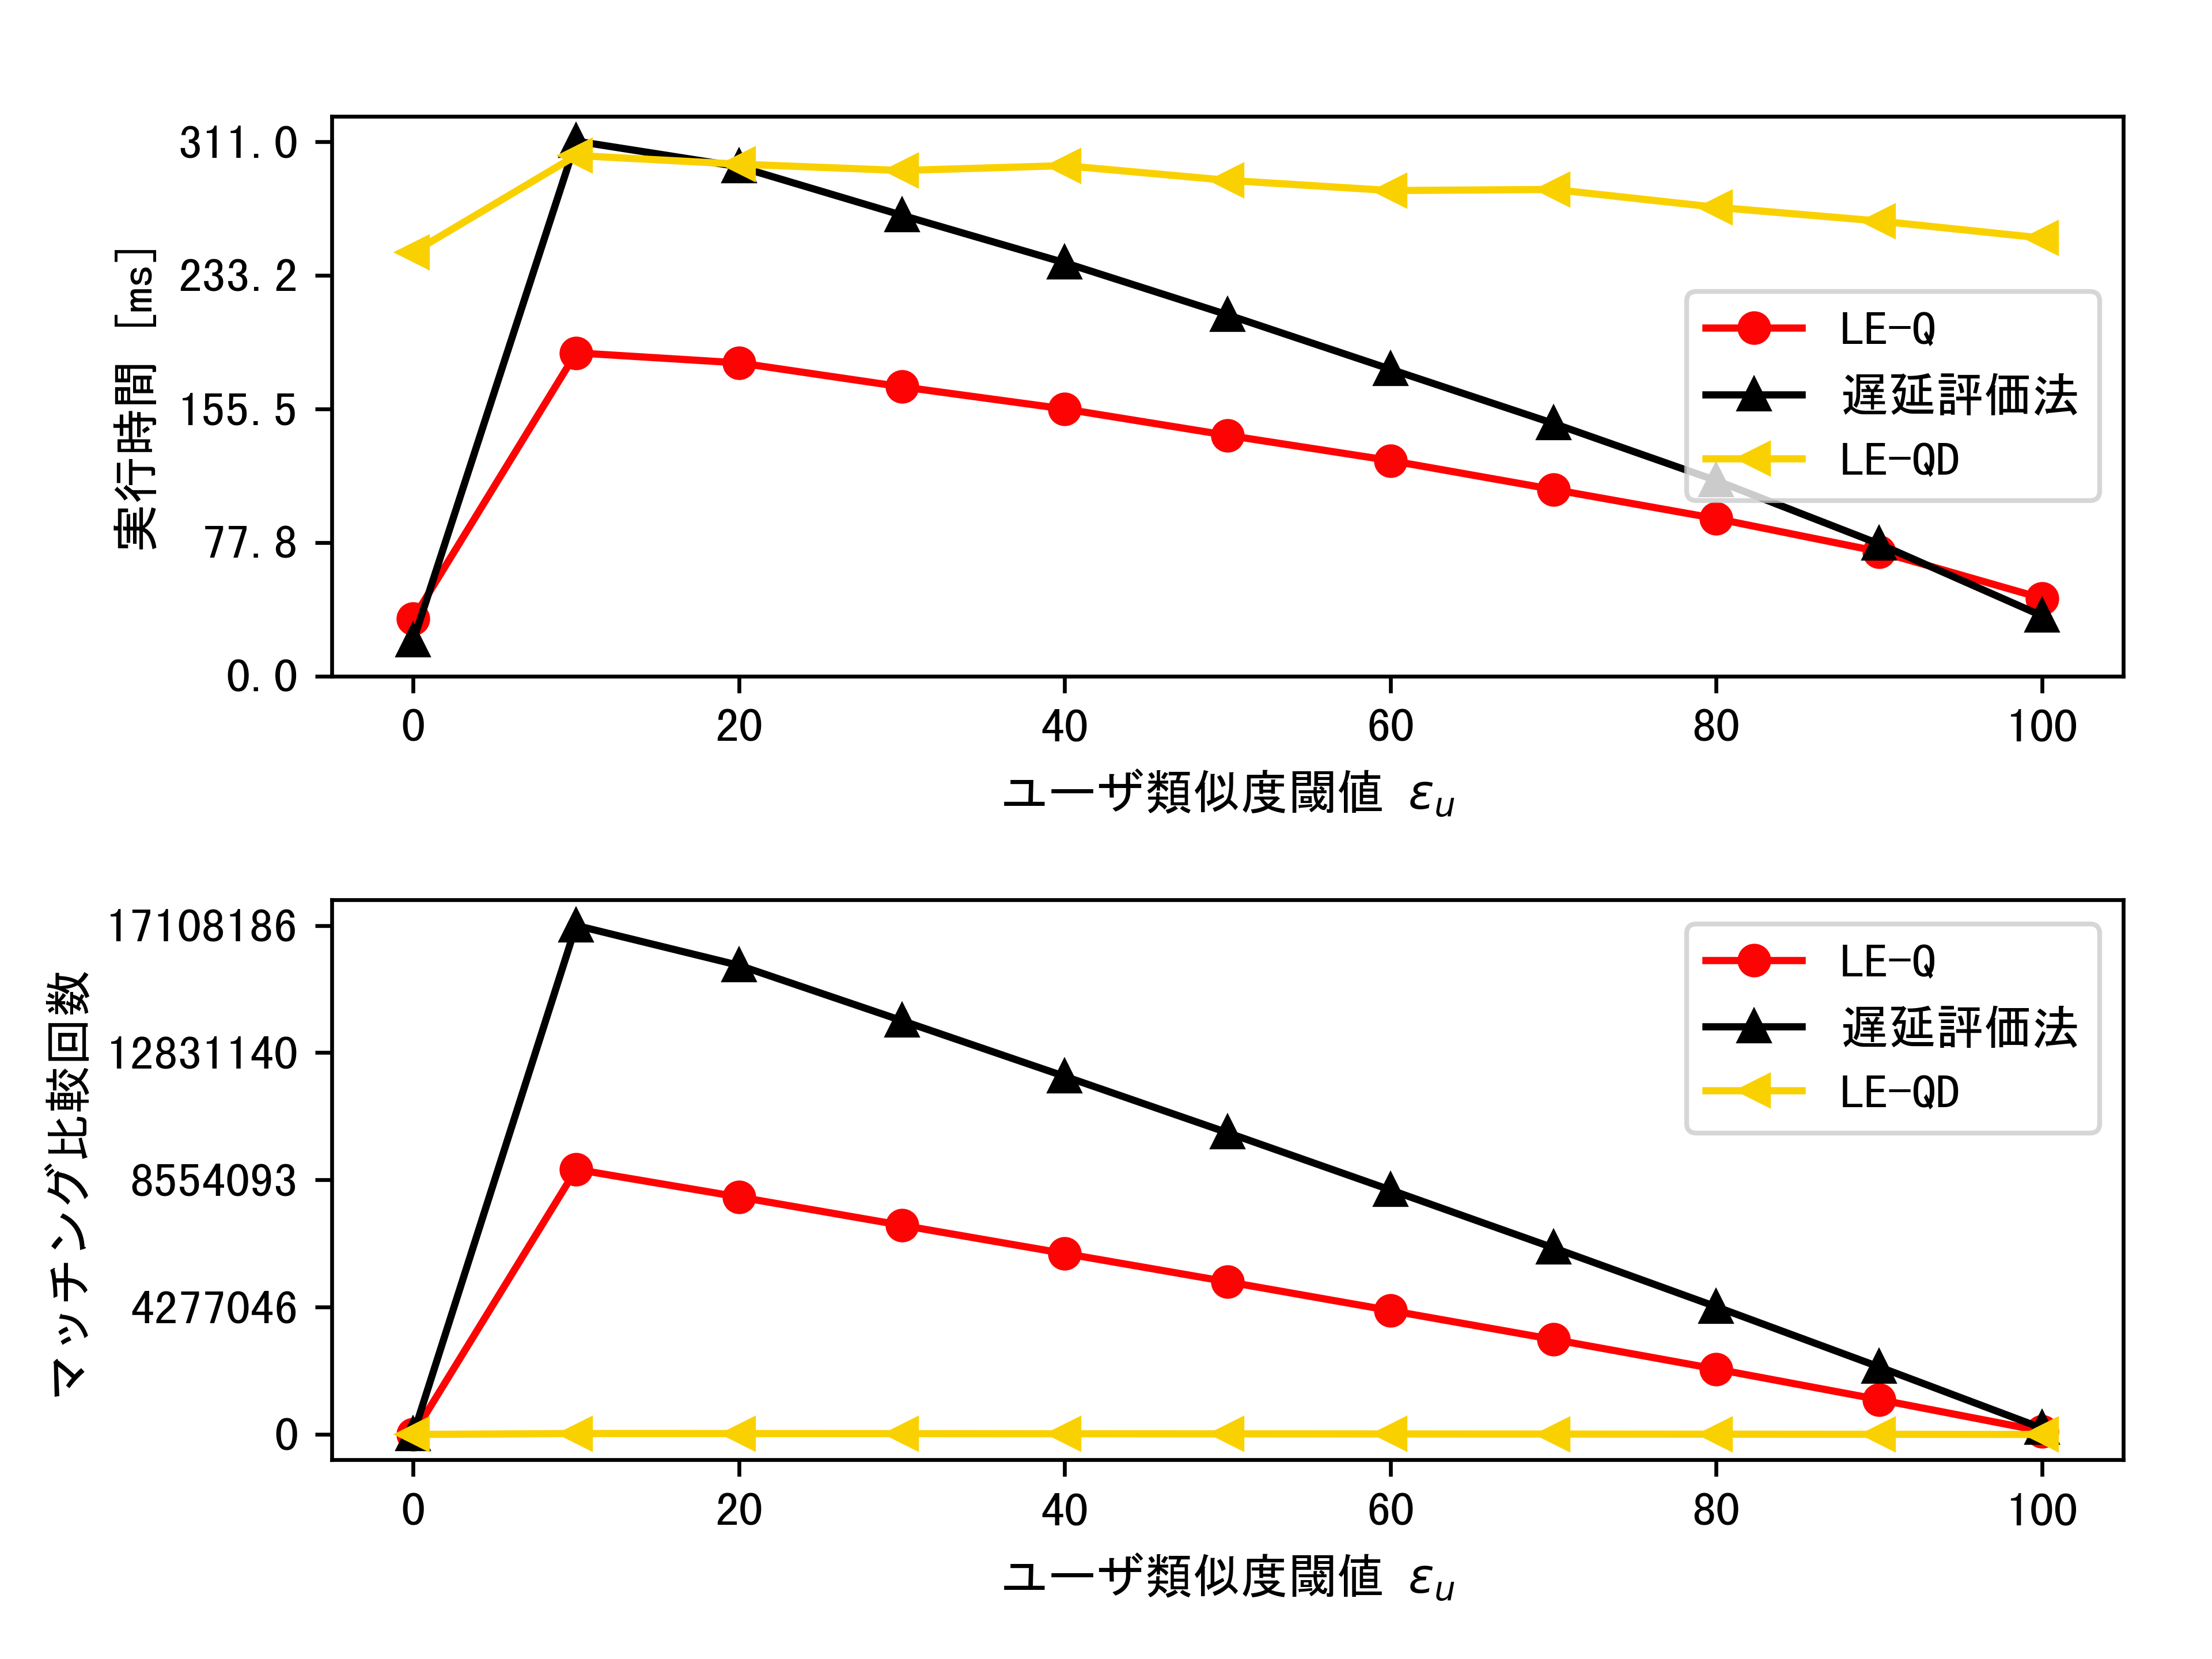
\includegraphics[width=8.3cm]{eimg/exp1_1.png}
    \caption{性能評価(人工データセット($p=0.1$))}
    \label{fig:exp1_art_1}
\end{figure}
\begin{figure}[H]
    \centering
    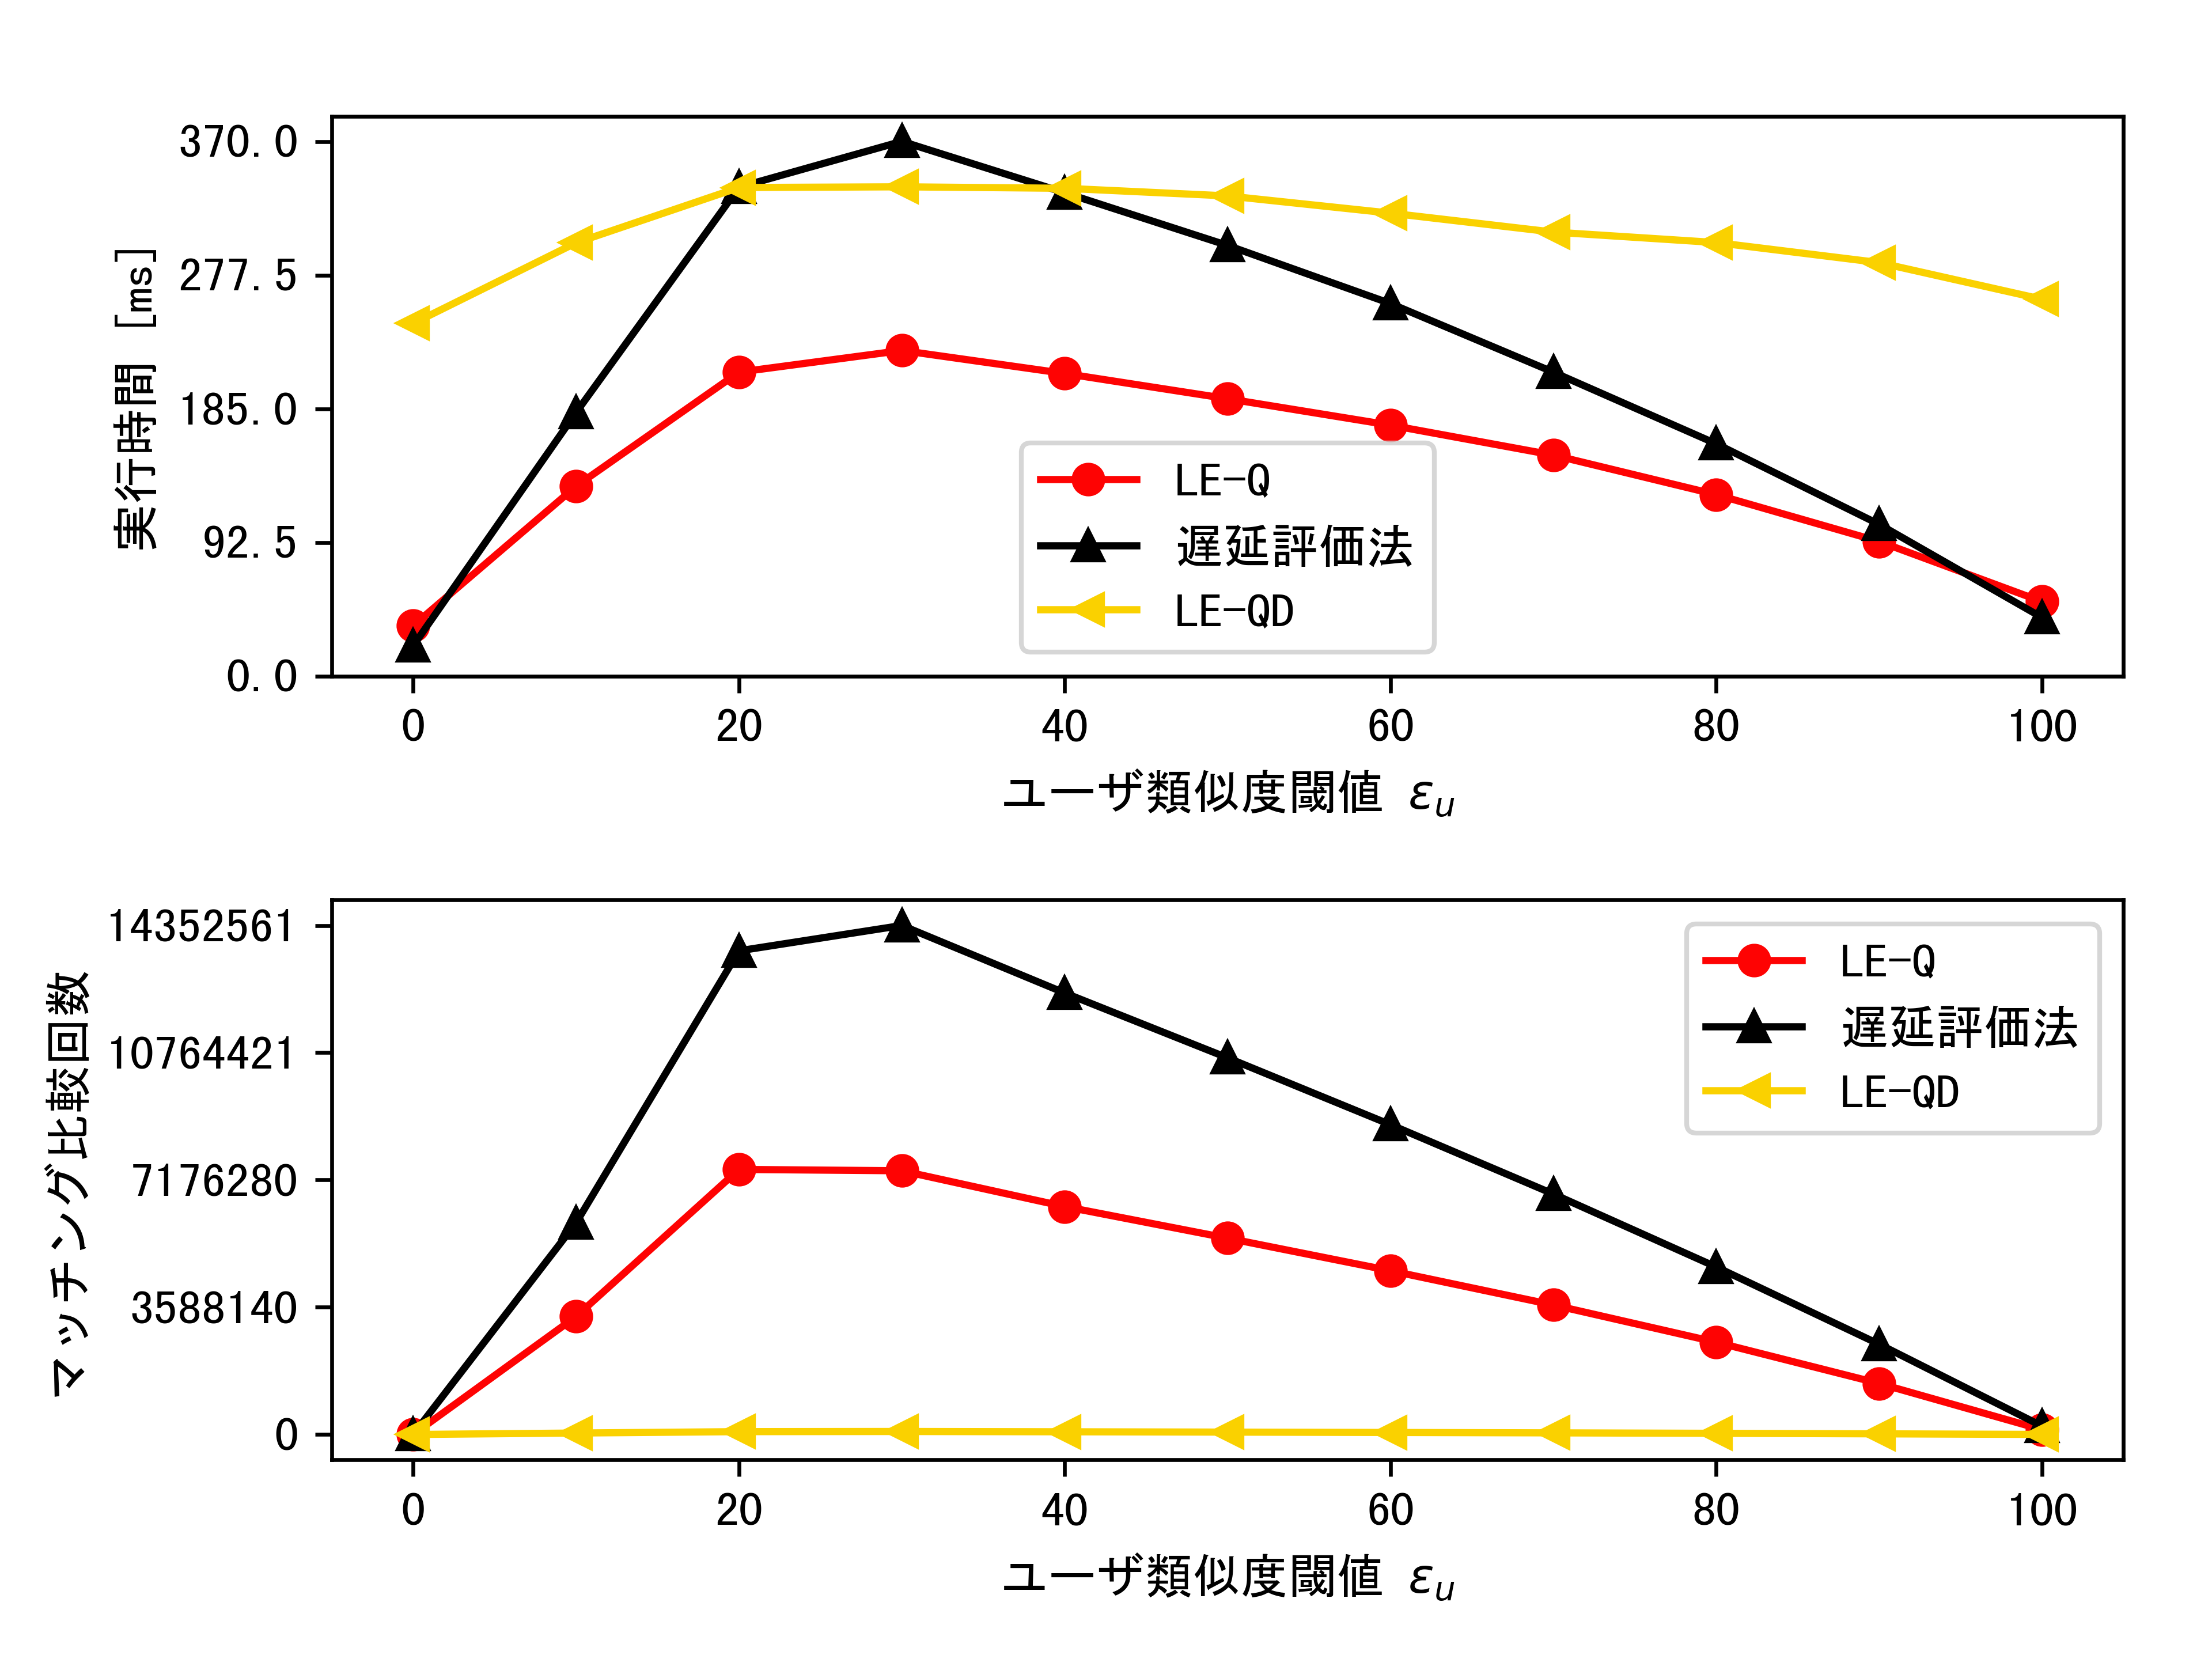
\includegraphics[width=8.3cm]{eimg/exp1_3.png}
    \caption{性能評価(人工データセット($p=0.3$))}
    \label{fig:exp1_art_3}
\end{figure}
\begin{figure}[H]
    \centering
    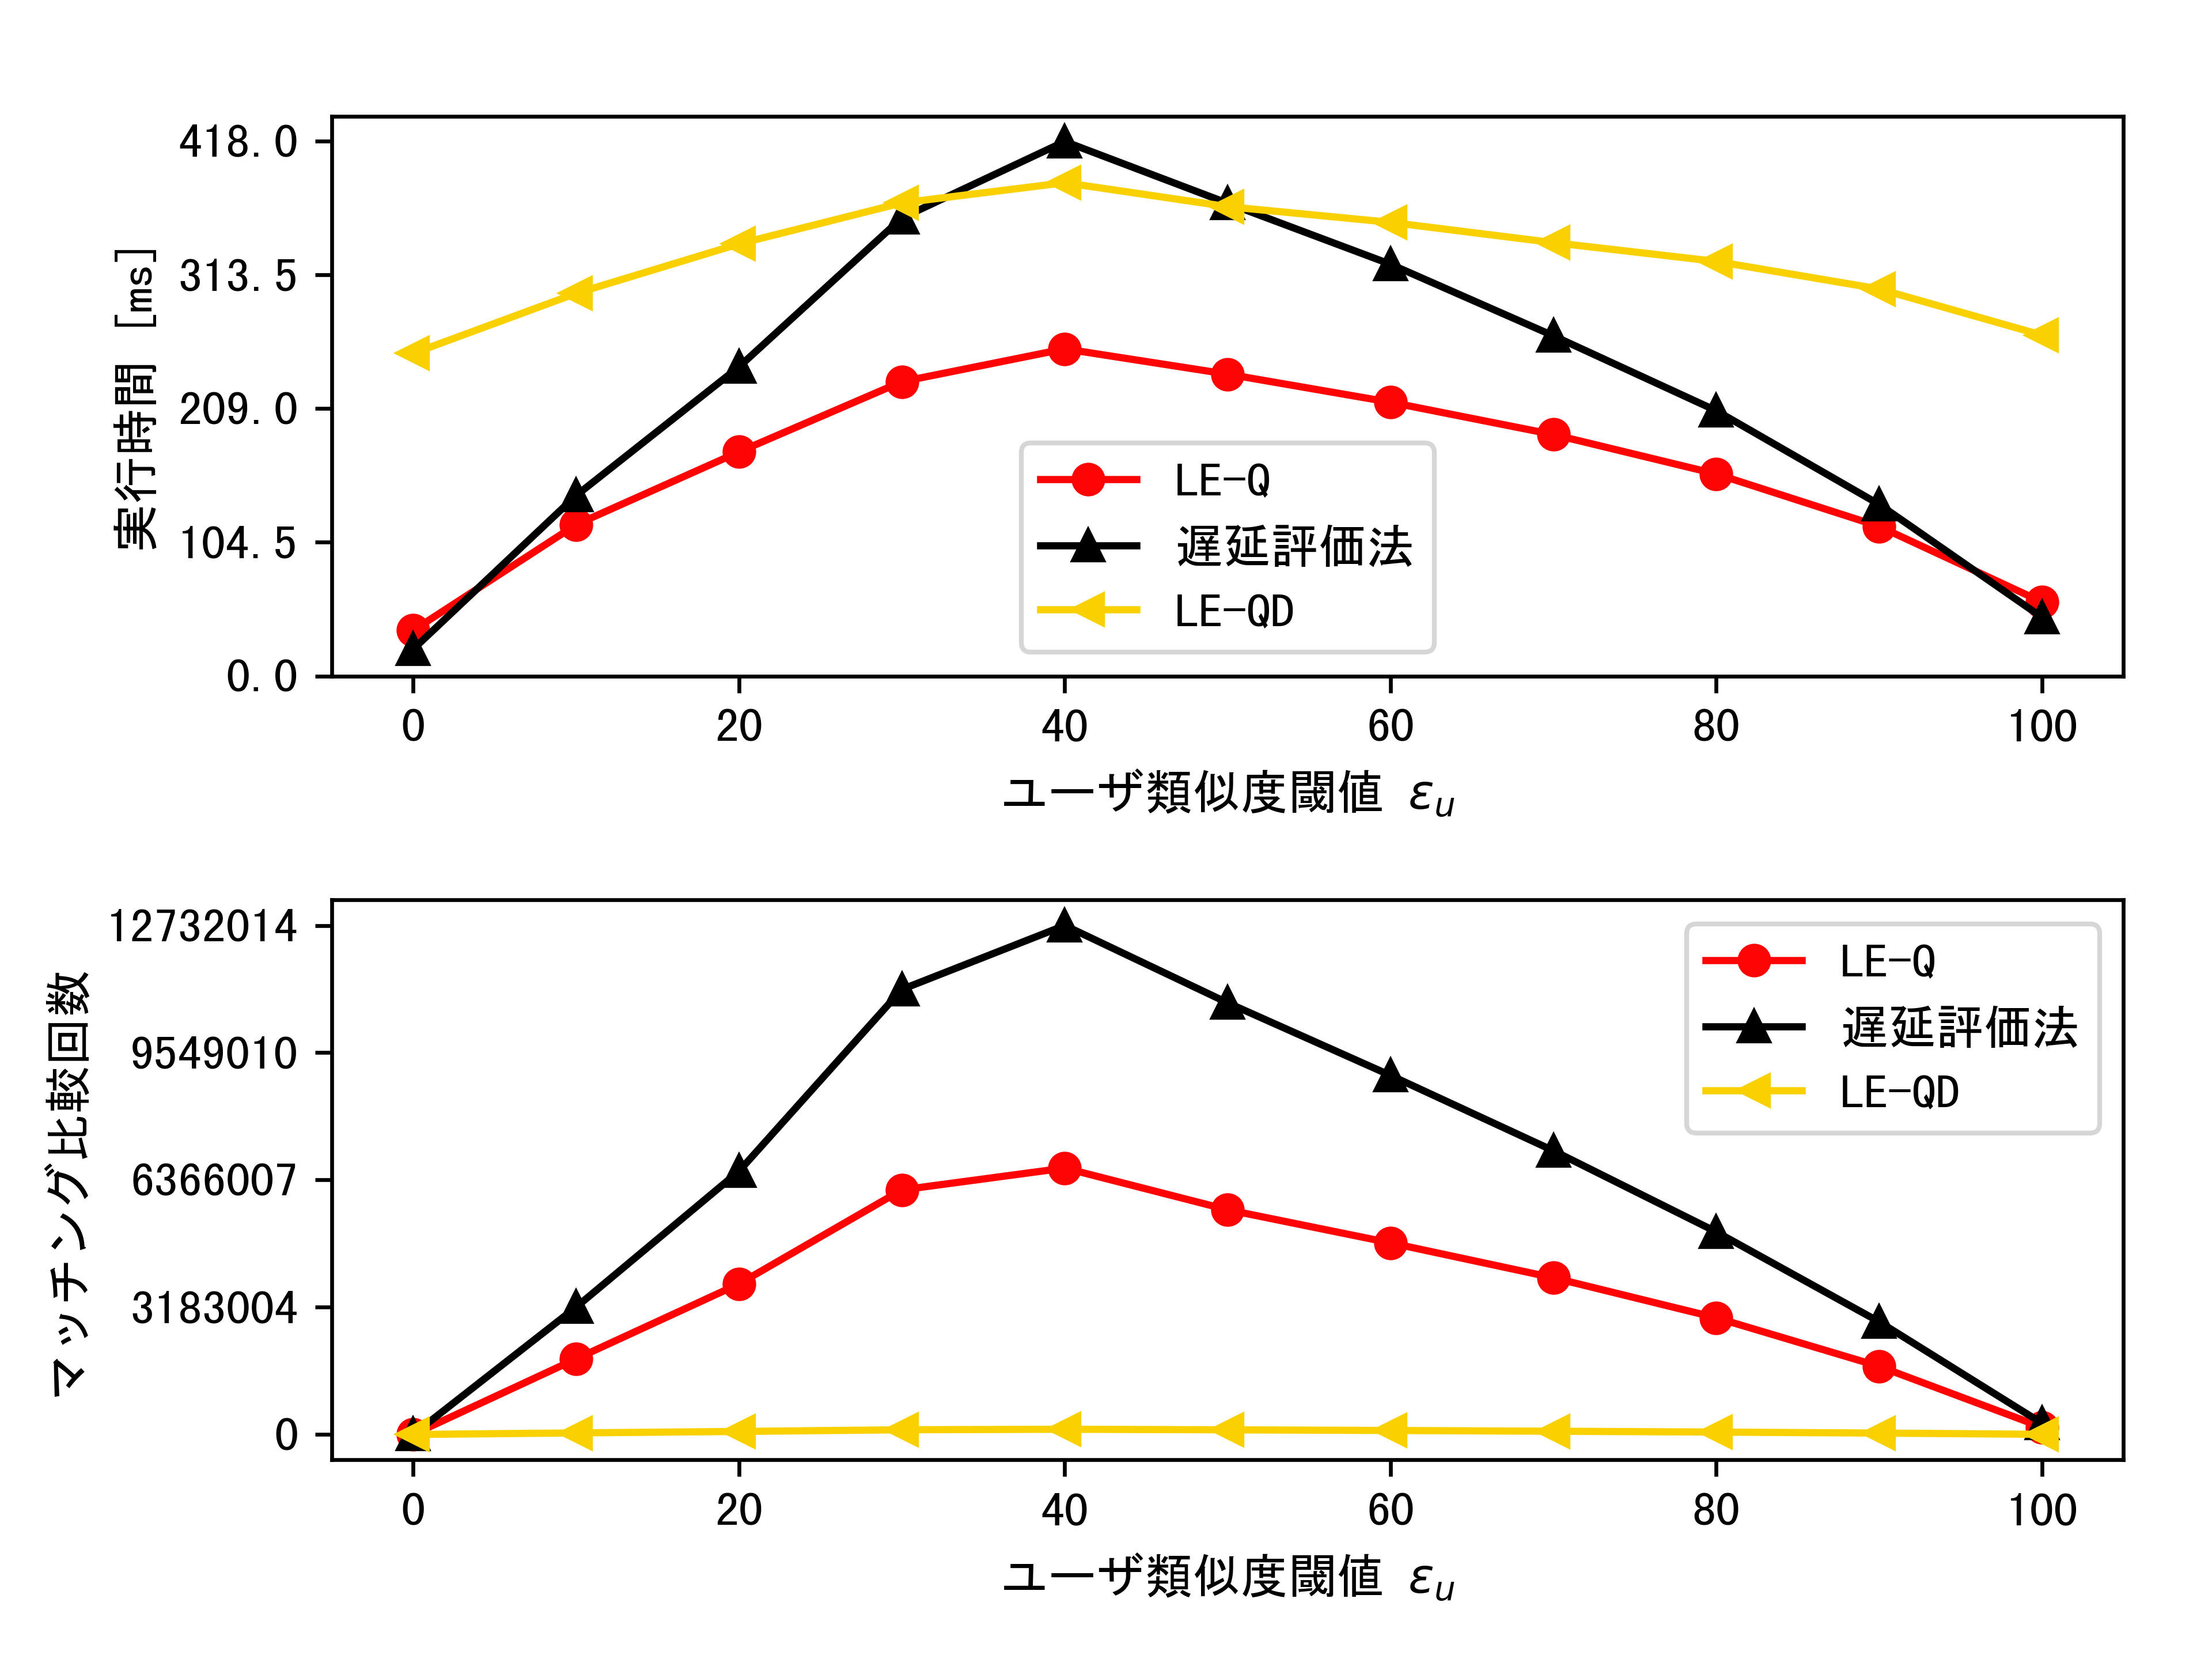
\includegraphics[width=8.3cm]{eimg/exp1_5.png}
    \caption{性能評価(人工データセット($p=0.5$))}
    \label{fig:exp1_art_5}
\end{figure}
\begin{figure}[H]
    \centering
    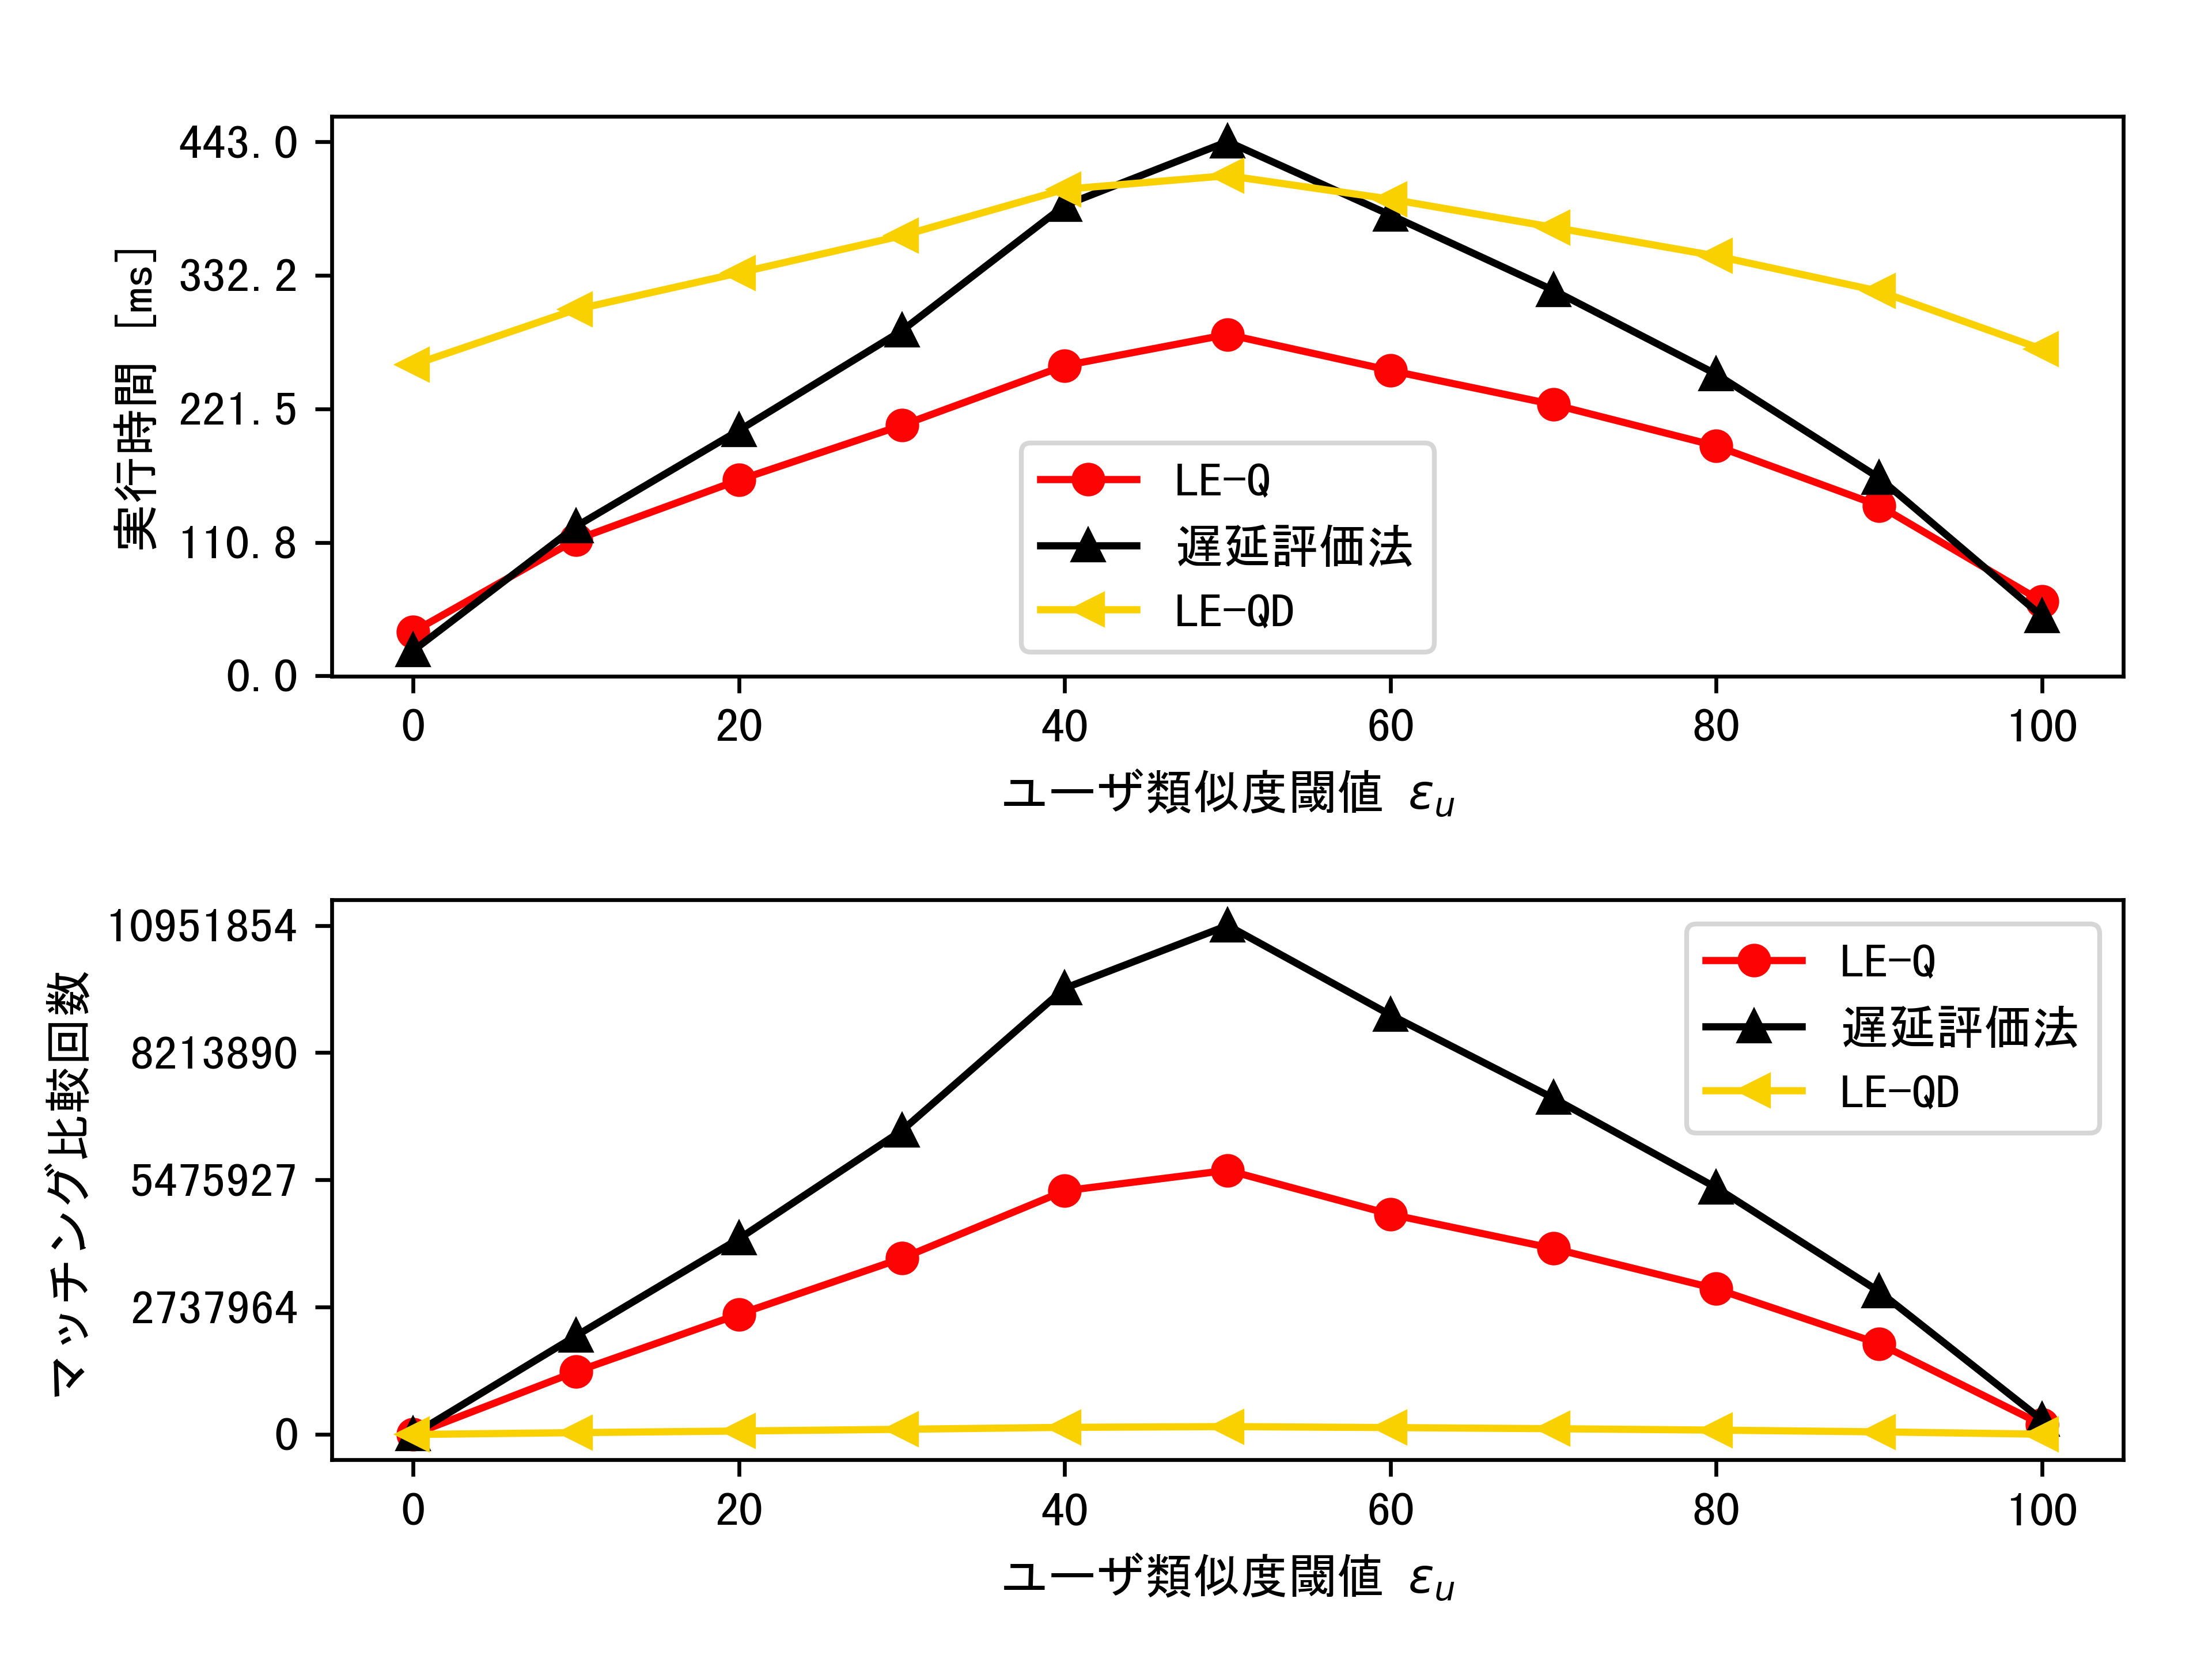
\includegraphics[width=8.3cm]{eimg/exp1_7.png}
    \caption{性能評価(人工データセット($p=0.7$))}
    \label{fig:exp1_art_7}
\end{figure}
\begin{figure}[H]
    \centering
    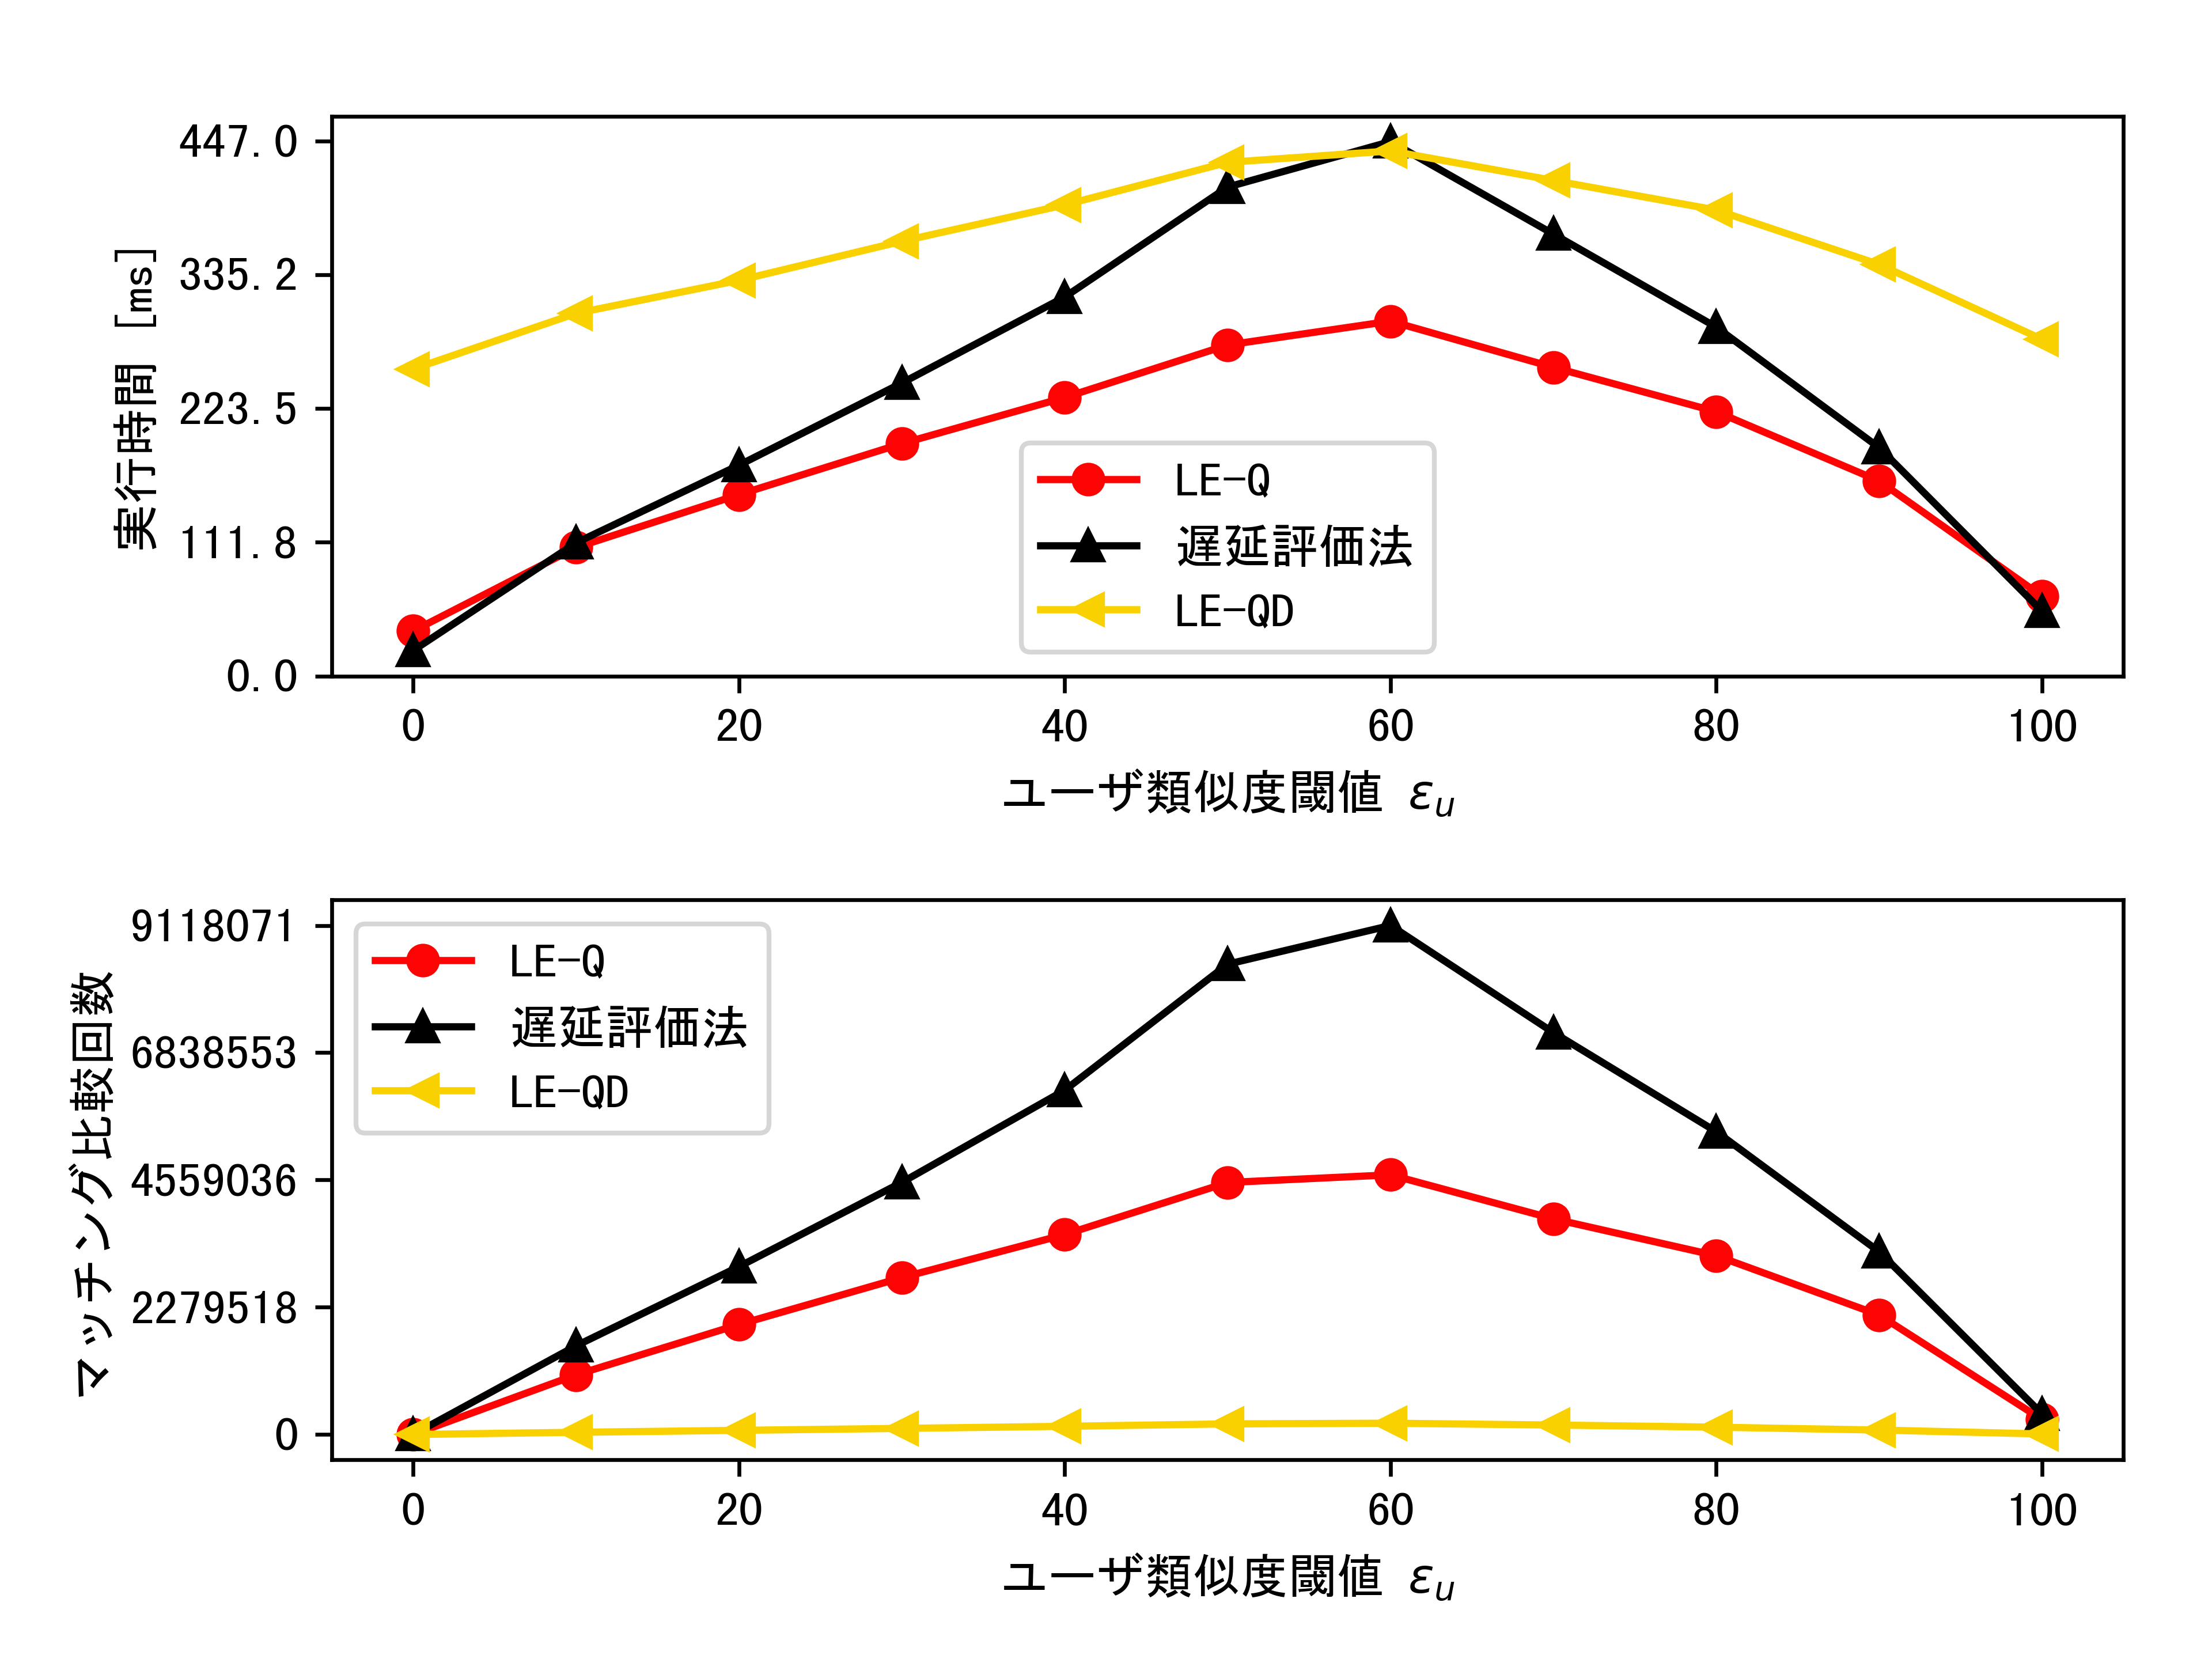
\includegraphics[width=8.3cm]{eimg/exp1_9.png}
    \caption{性能評価(人工データセット($p=0.9$))}
    \label{fig:exp1_art_9}
\end{figure}



\section{マッチング順序の評価}
\ref{exp1}節の実験からLE-QDよりもLE-Qの方が優れていると考えられるため,本実験ではLE-Qを対象とする.
\ref{order_matching}節で示したとおりマッチング順序に関しては新しいテキストから優先してマッチング判定をすることが効率的であると考えられるが,この優位性が転置インデクスを用いたアルゴリズムでも確認できるかを調べる.そのためにLE-Qにおけるマッチング処理を古いテキスト優先のマッチング処理に置き換え,全ユーザの類似性を各時刻すべてにおいて求める実験を行った.
人工データセットにおける実験結果を図\ref{fig:exp2}に示した.
結果より,新しいテキストから優先的にマッチングする方が実行時間が短縮され効果的であることが示された.これは新しいテキスト優先にすることでマッチング比較回数を削減することが出来た影響であると考える.

\begin{figure}[H]
    \centering
    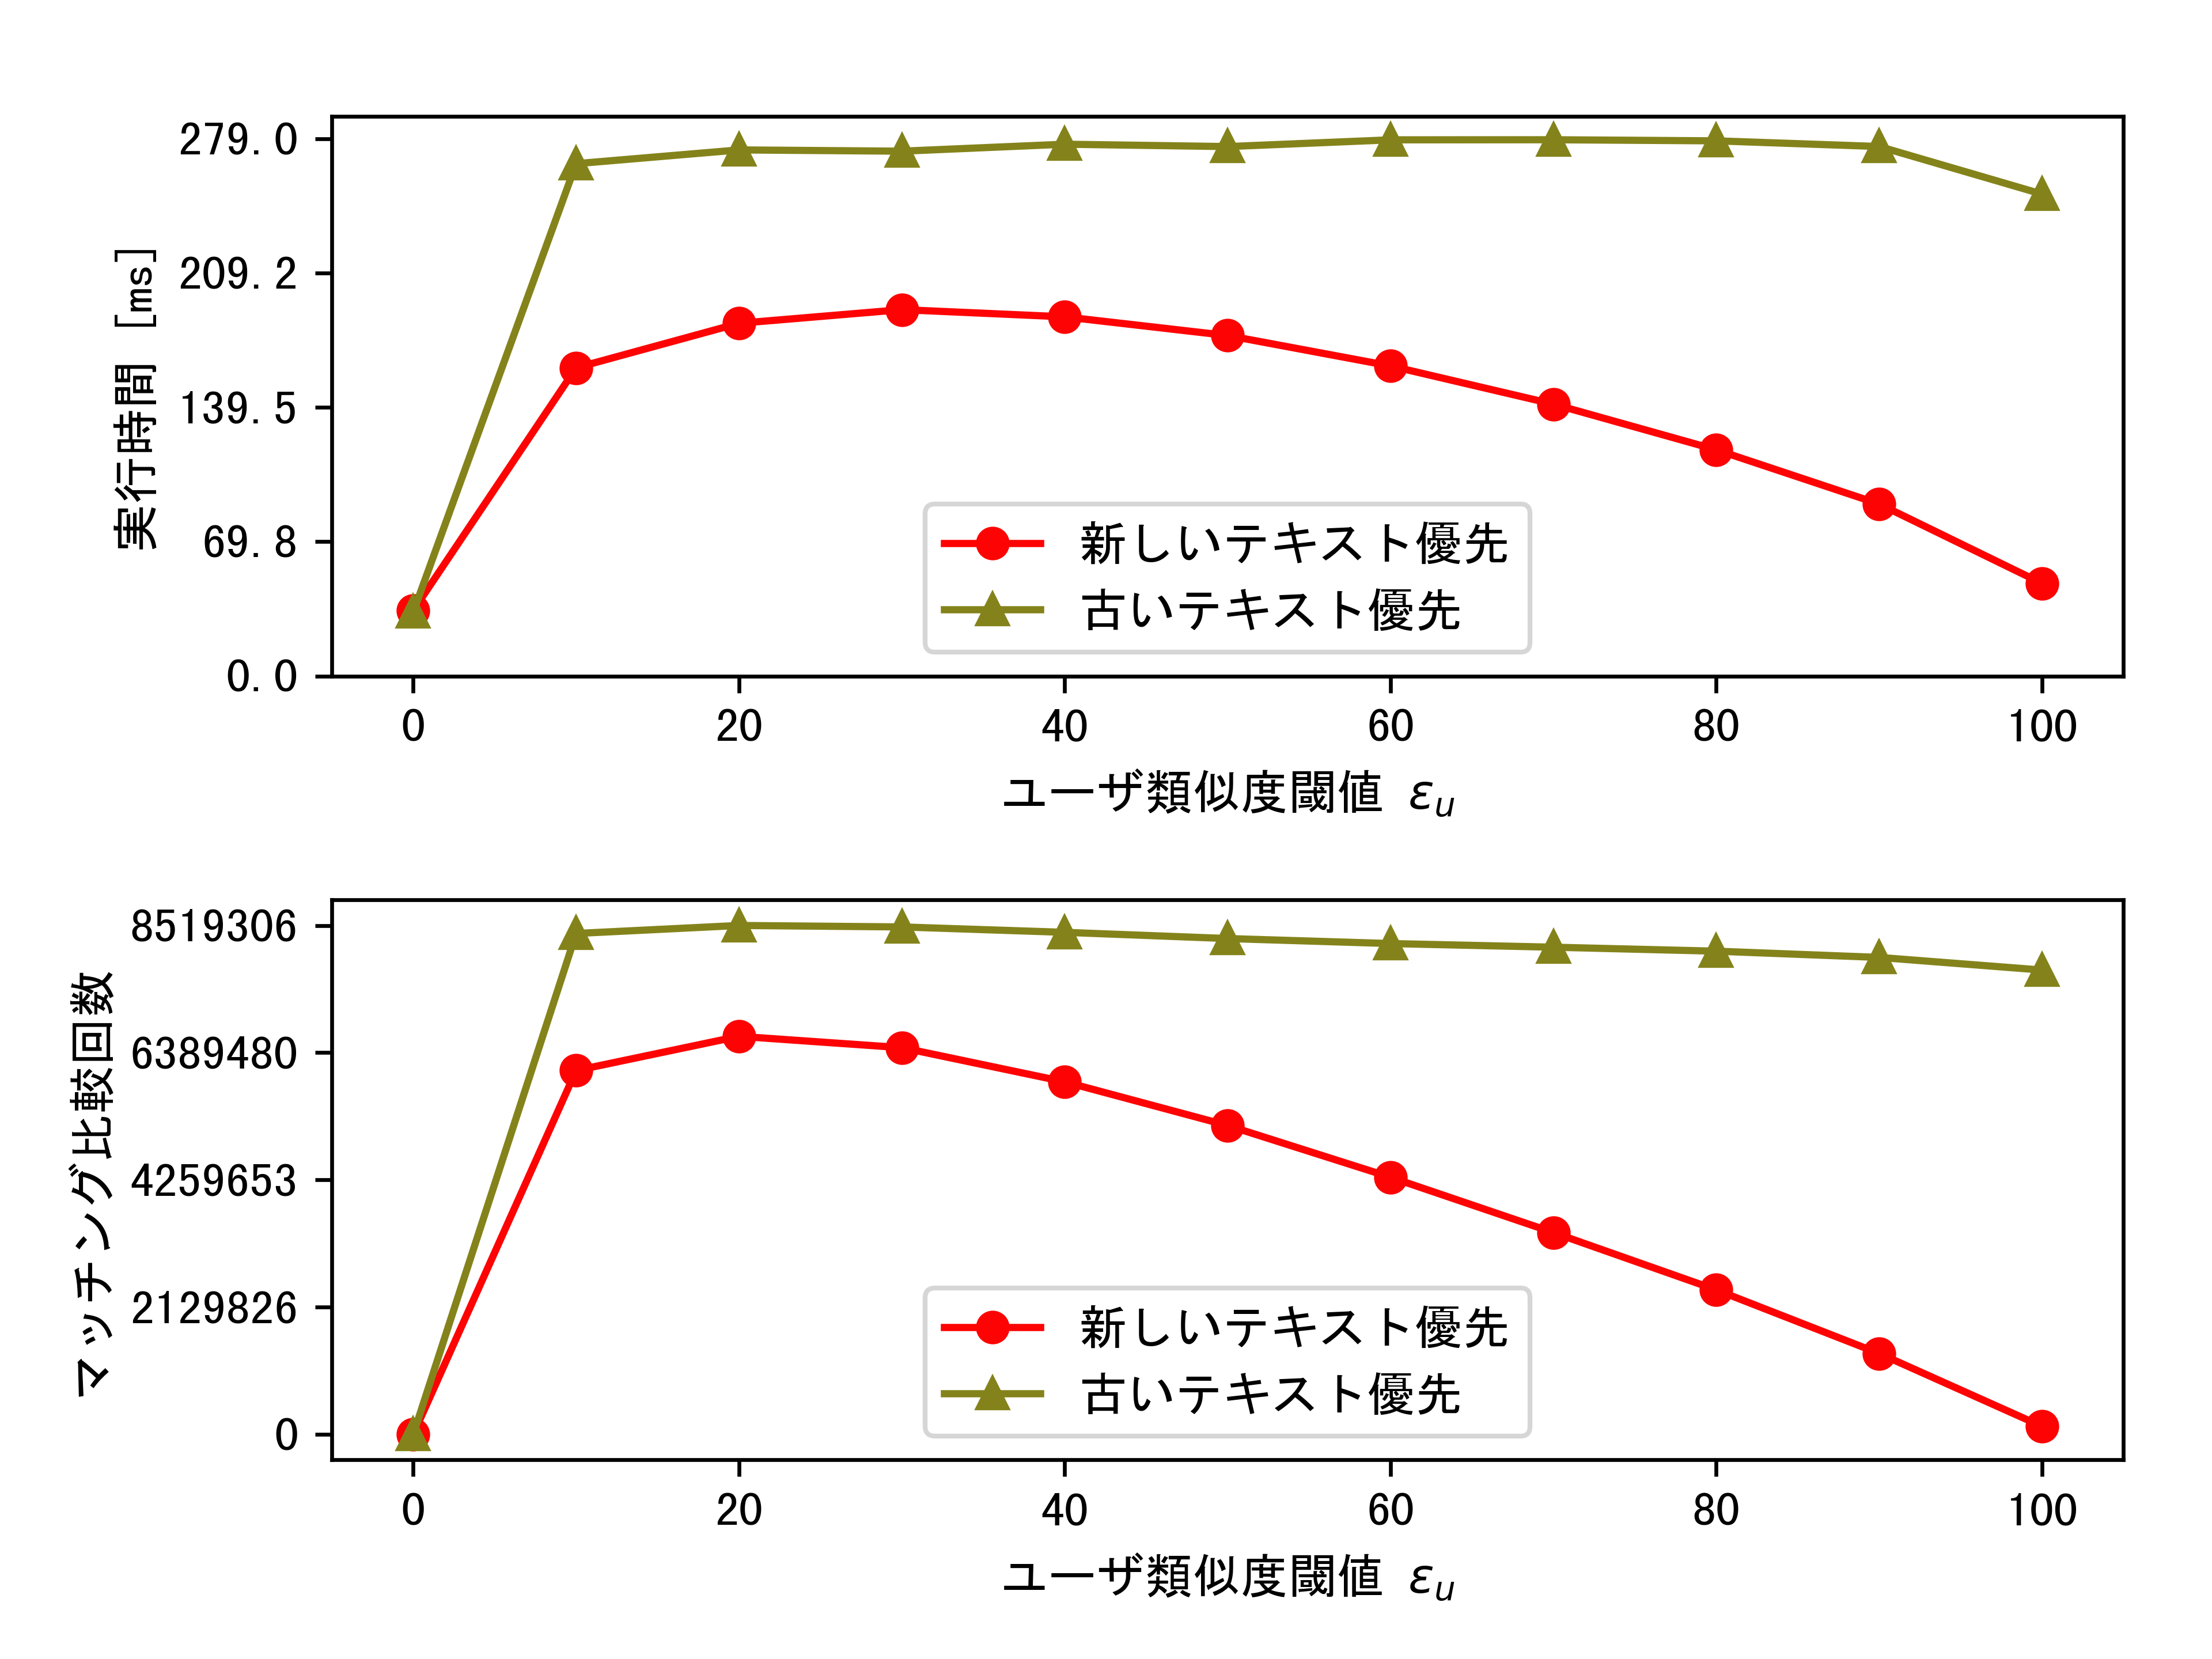
\includegraphics[width=8.3cm]{eimg/exp2.png}
    \caption{LE-Qのマッチング順序の優位性評価(人工データセット($p=0.96^{(i-1)}$))}
    \label{fig:exp2}
\end{figure}
CoPhIRデータセットにおける実験結果を図\ref{fig:exp2_c}に示した.
図\ref{fig:exp2_c}は人工データによる実験と同様の結果を示し,テキストのマッチング順序として新しいテキストから優先することは有効であると確認できた.
\begin{figure}[H]
    \centering
    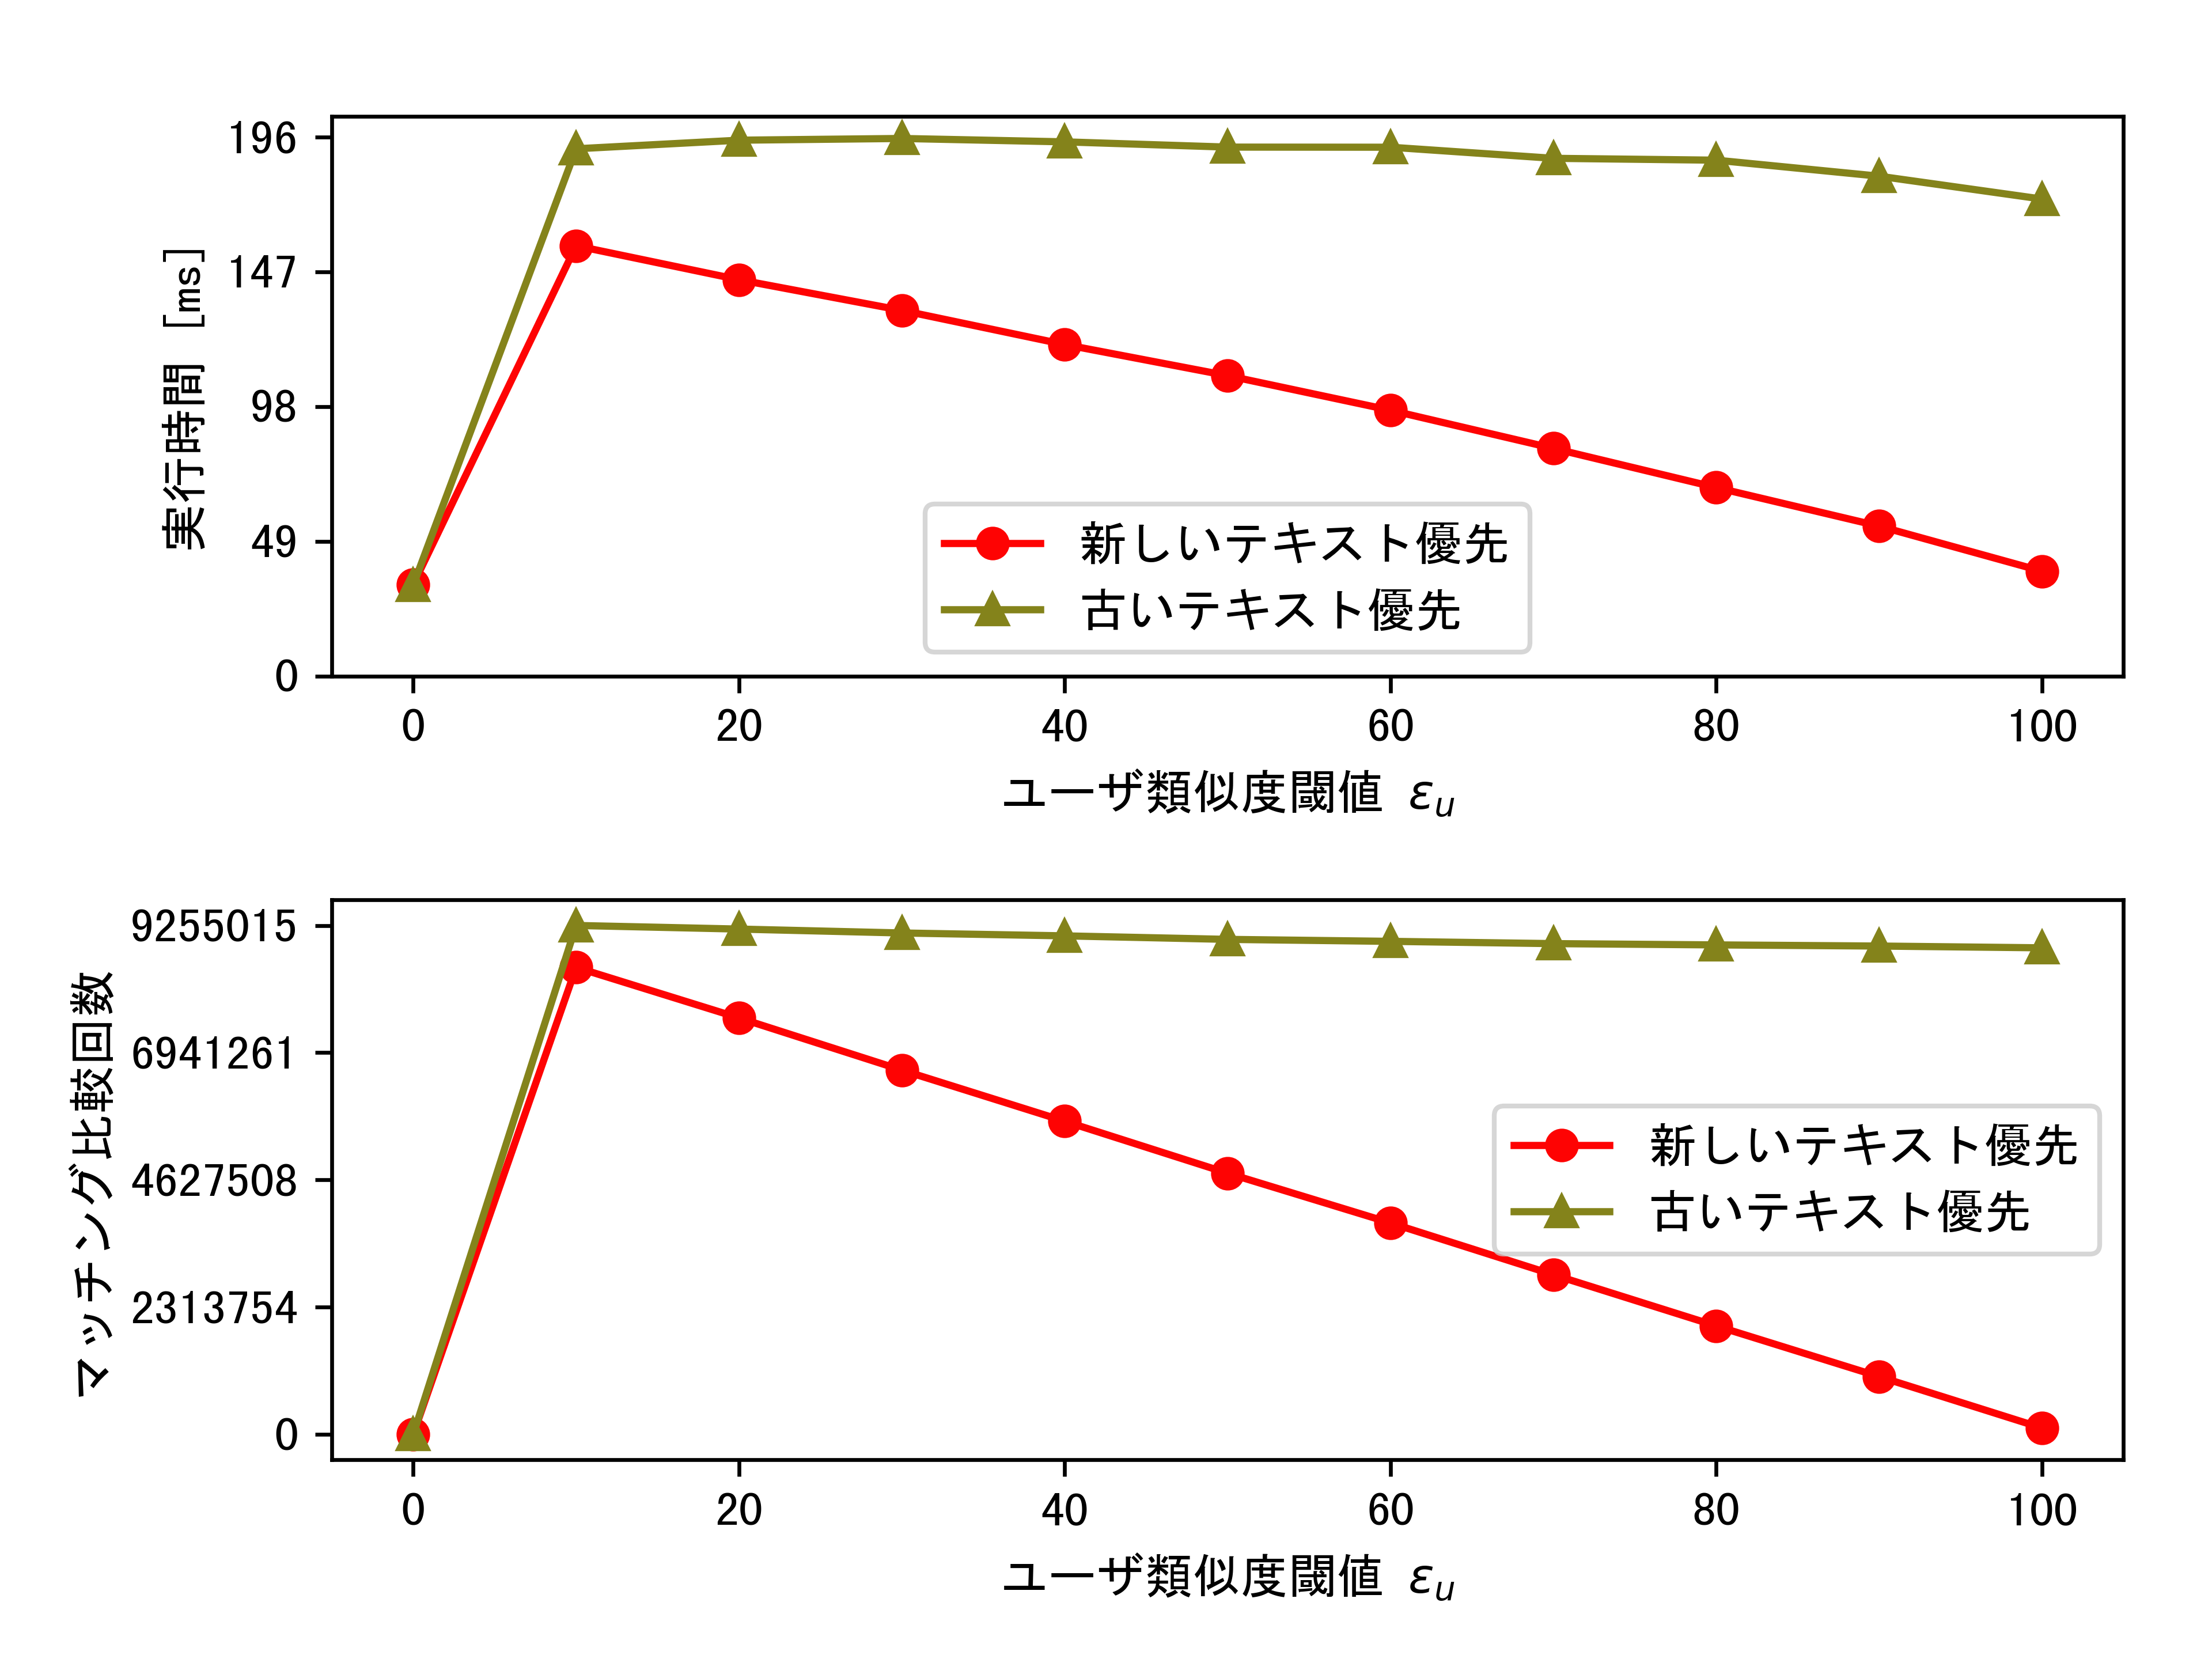
\includegraphics[width=8.3cm]{eimg/exp2_c.png}
    \caption{LE-Qのマッチング順序の優位性評価(CoPhIRデータセット)}
    \label{fig:exp2_c}
\end{figure}

人工データセットにおける$p$を固定した場合の実験結果を図\ref{fig:exp2_1},図\ref{fig:exp2_3},図\ref{fig:exp2_5},図\ref{fig:exp2_7},図\ref{fig:exp2_9}に示した.
$p$の値によらずマッチングには新しいテキストを優先することが効果的であることが示された.

\begin{figure}[H]
    \centering
    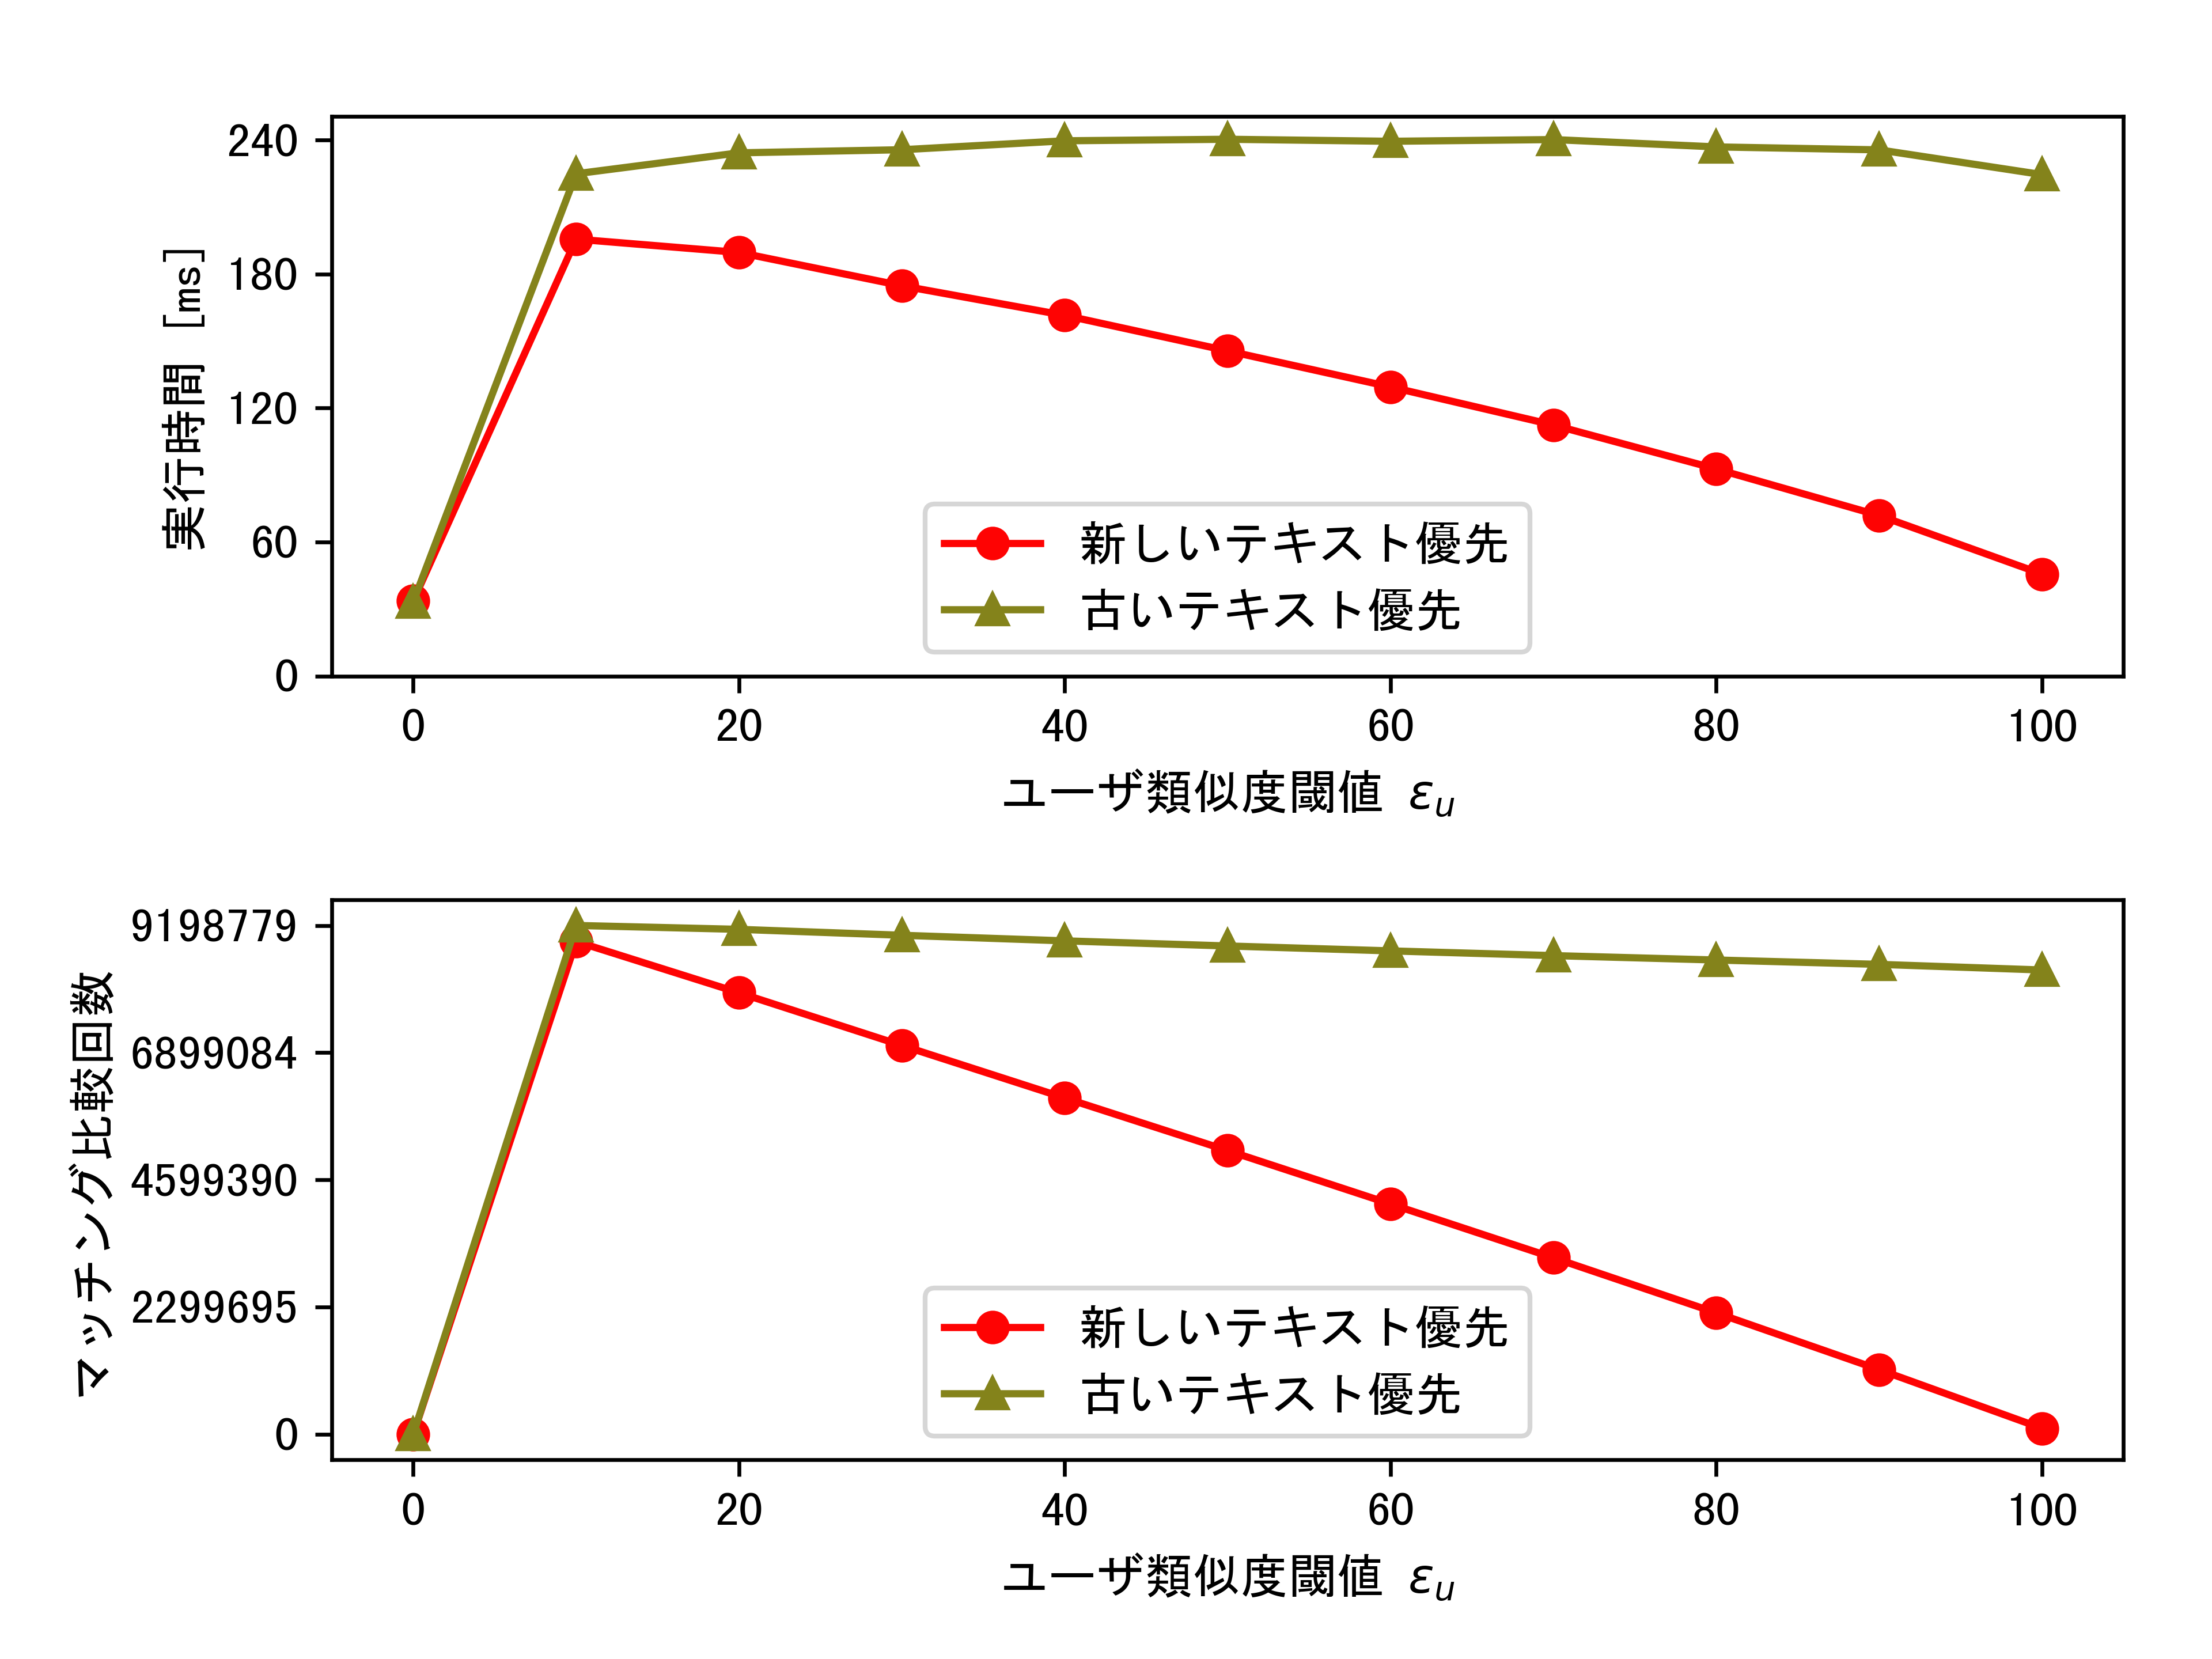
\includegraphics[width=8.3cm]{eimg/exp2_1.png}
    \caption{LE-Qのマッチング順序の優位性評価(人工データセット($p=0.1$))}
    \label{fig:exp2_1}
\end{figure}
\begin{figure}[H]
    \centering
    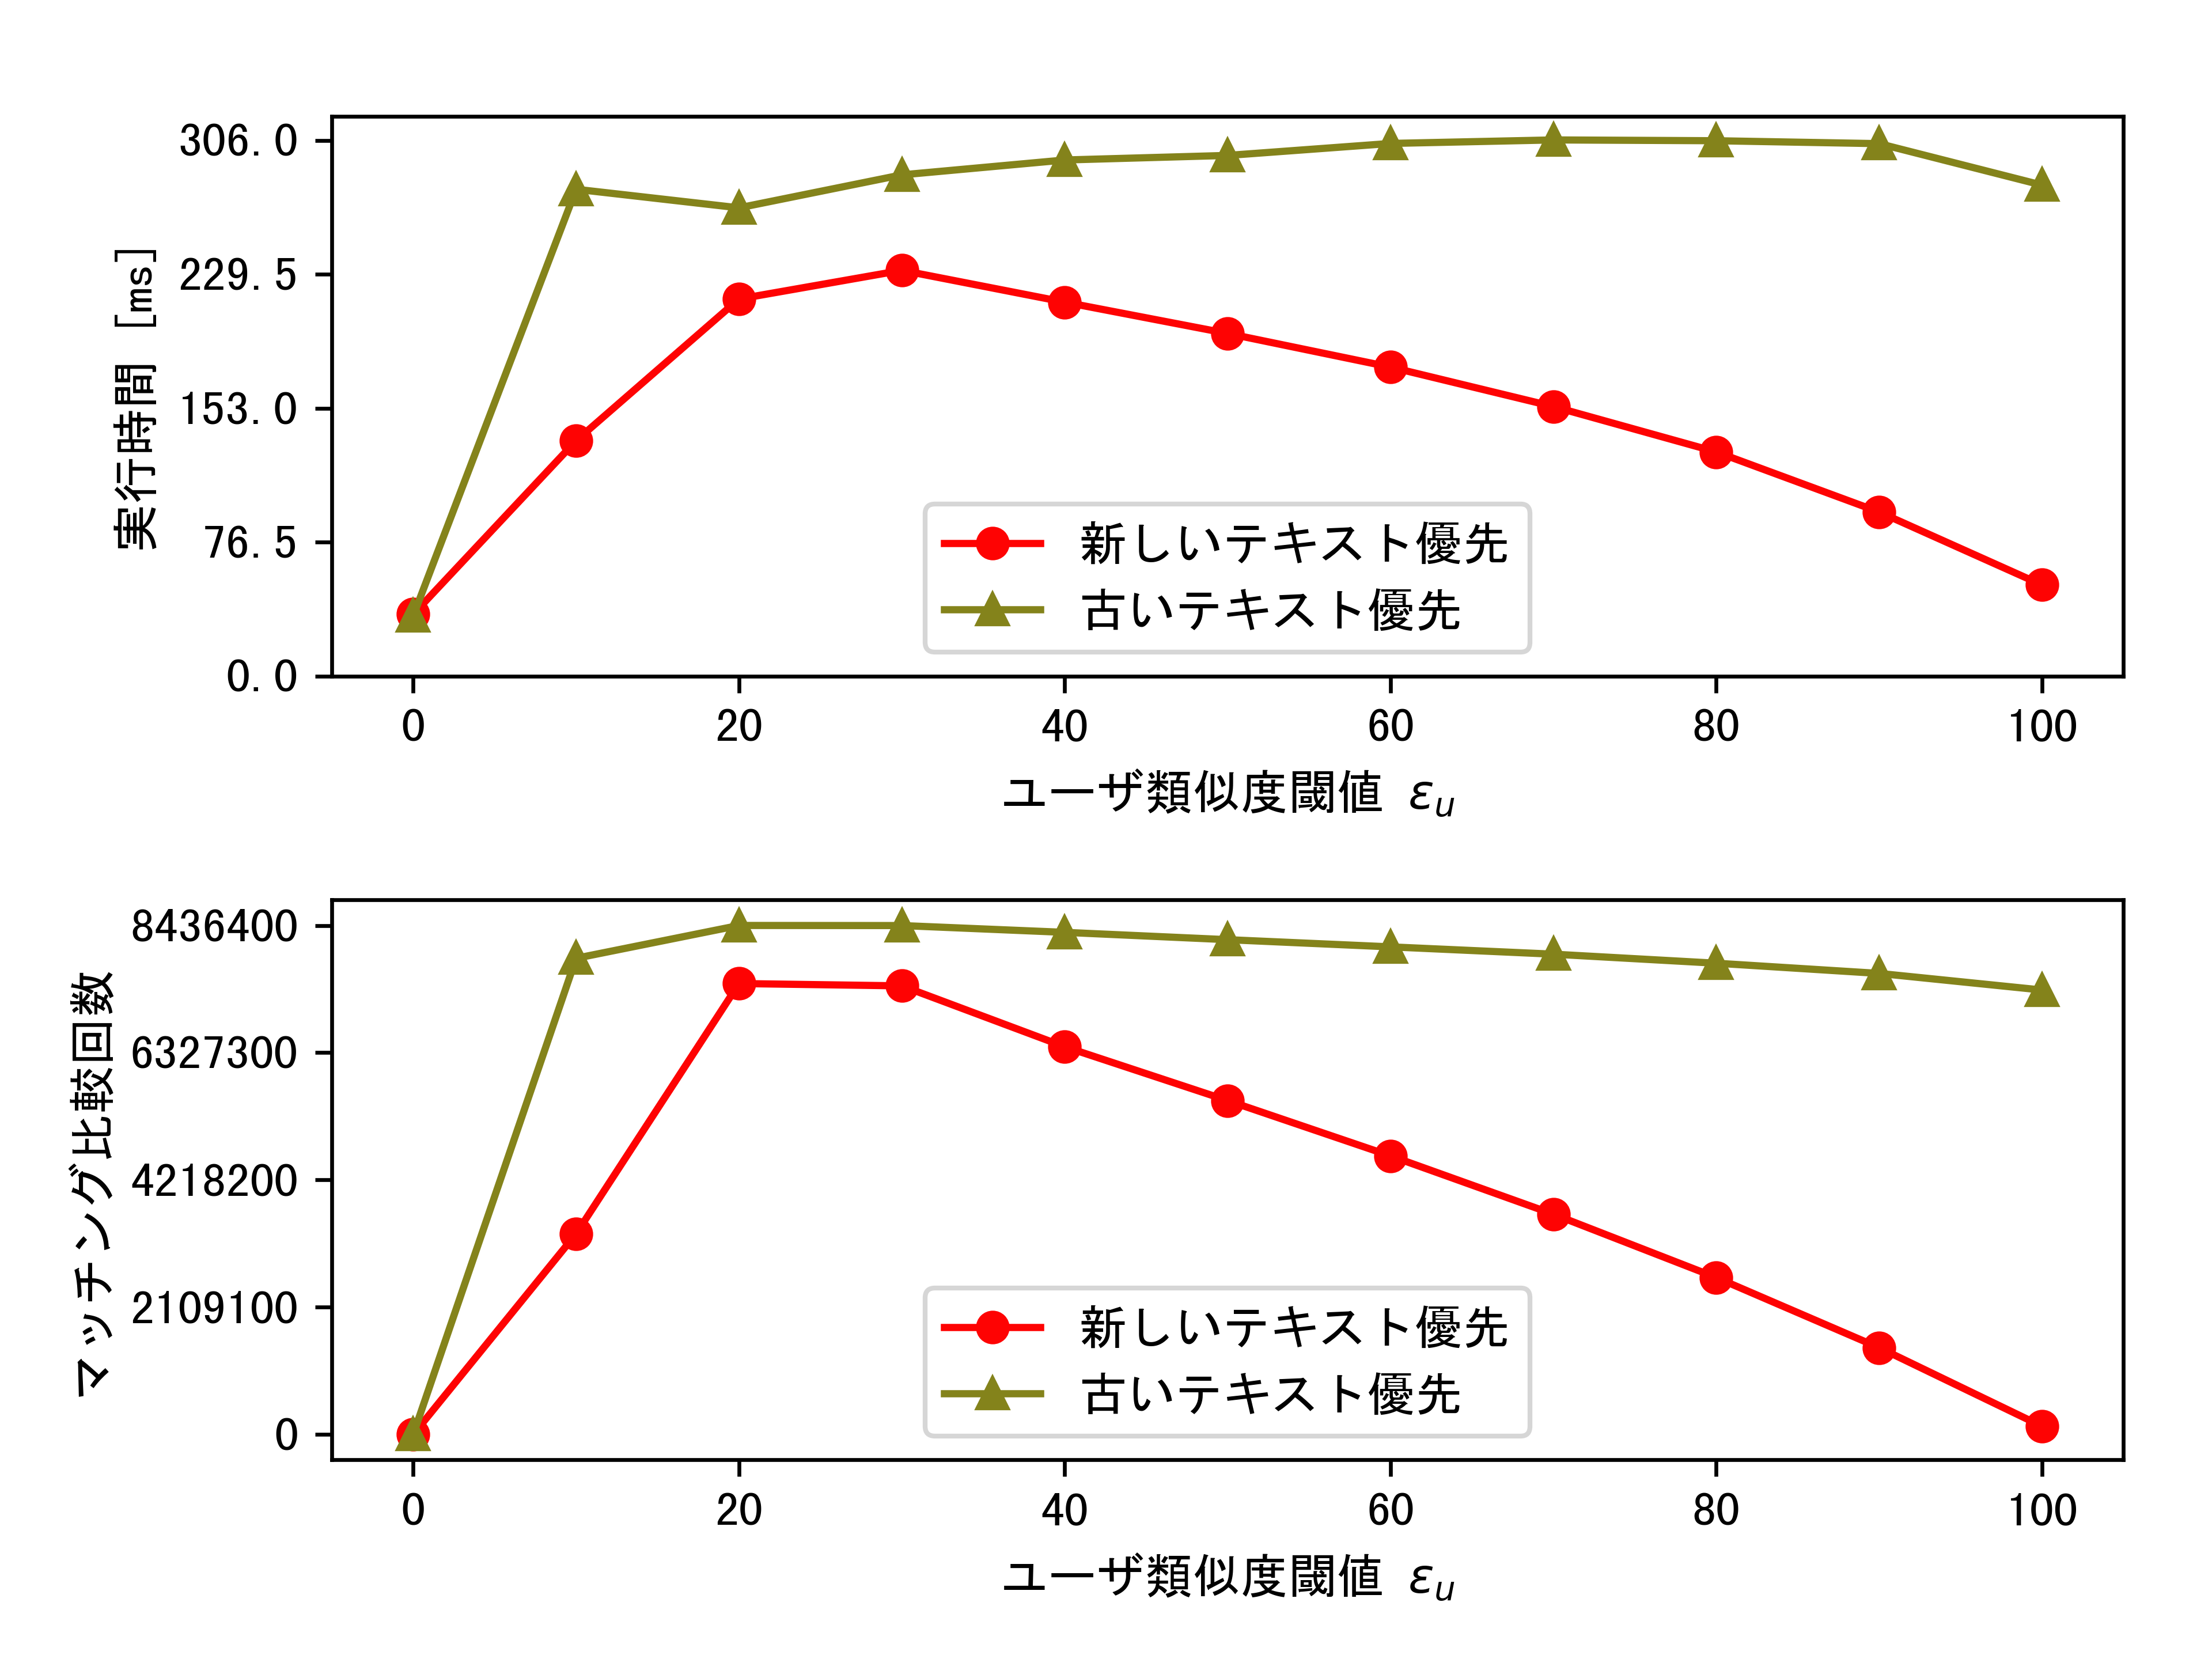
\includegraphics[width=8.3cm]{eimg/exp2_3.png}
    \caption{LE-Qのマッチング順序の優位性評価(人工データセット($p=0.3$))}
    \label{fig:exp2_3}
\end{figure}
\begin{figure}[H]
    \centering
    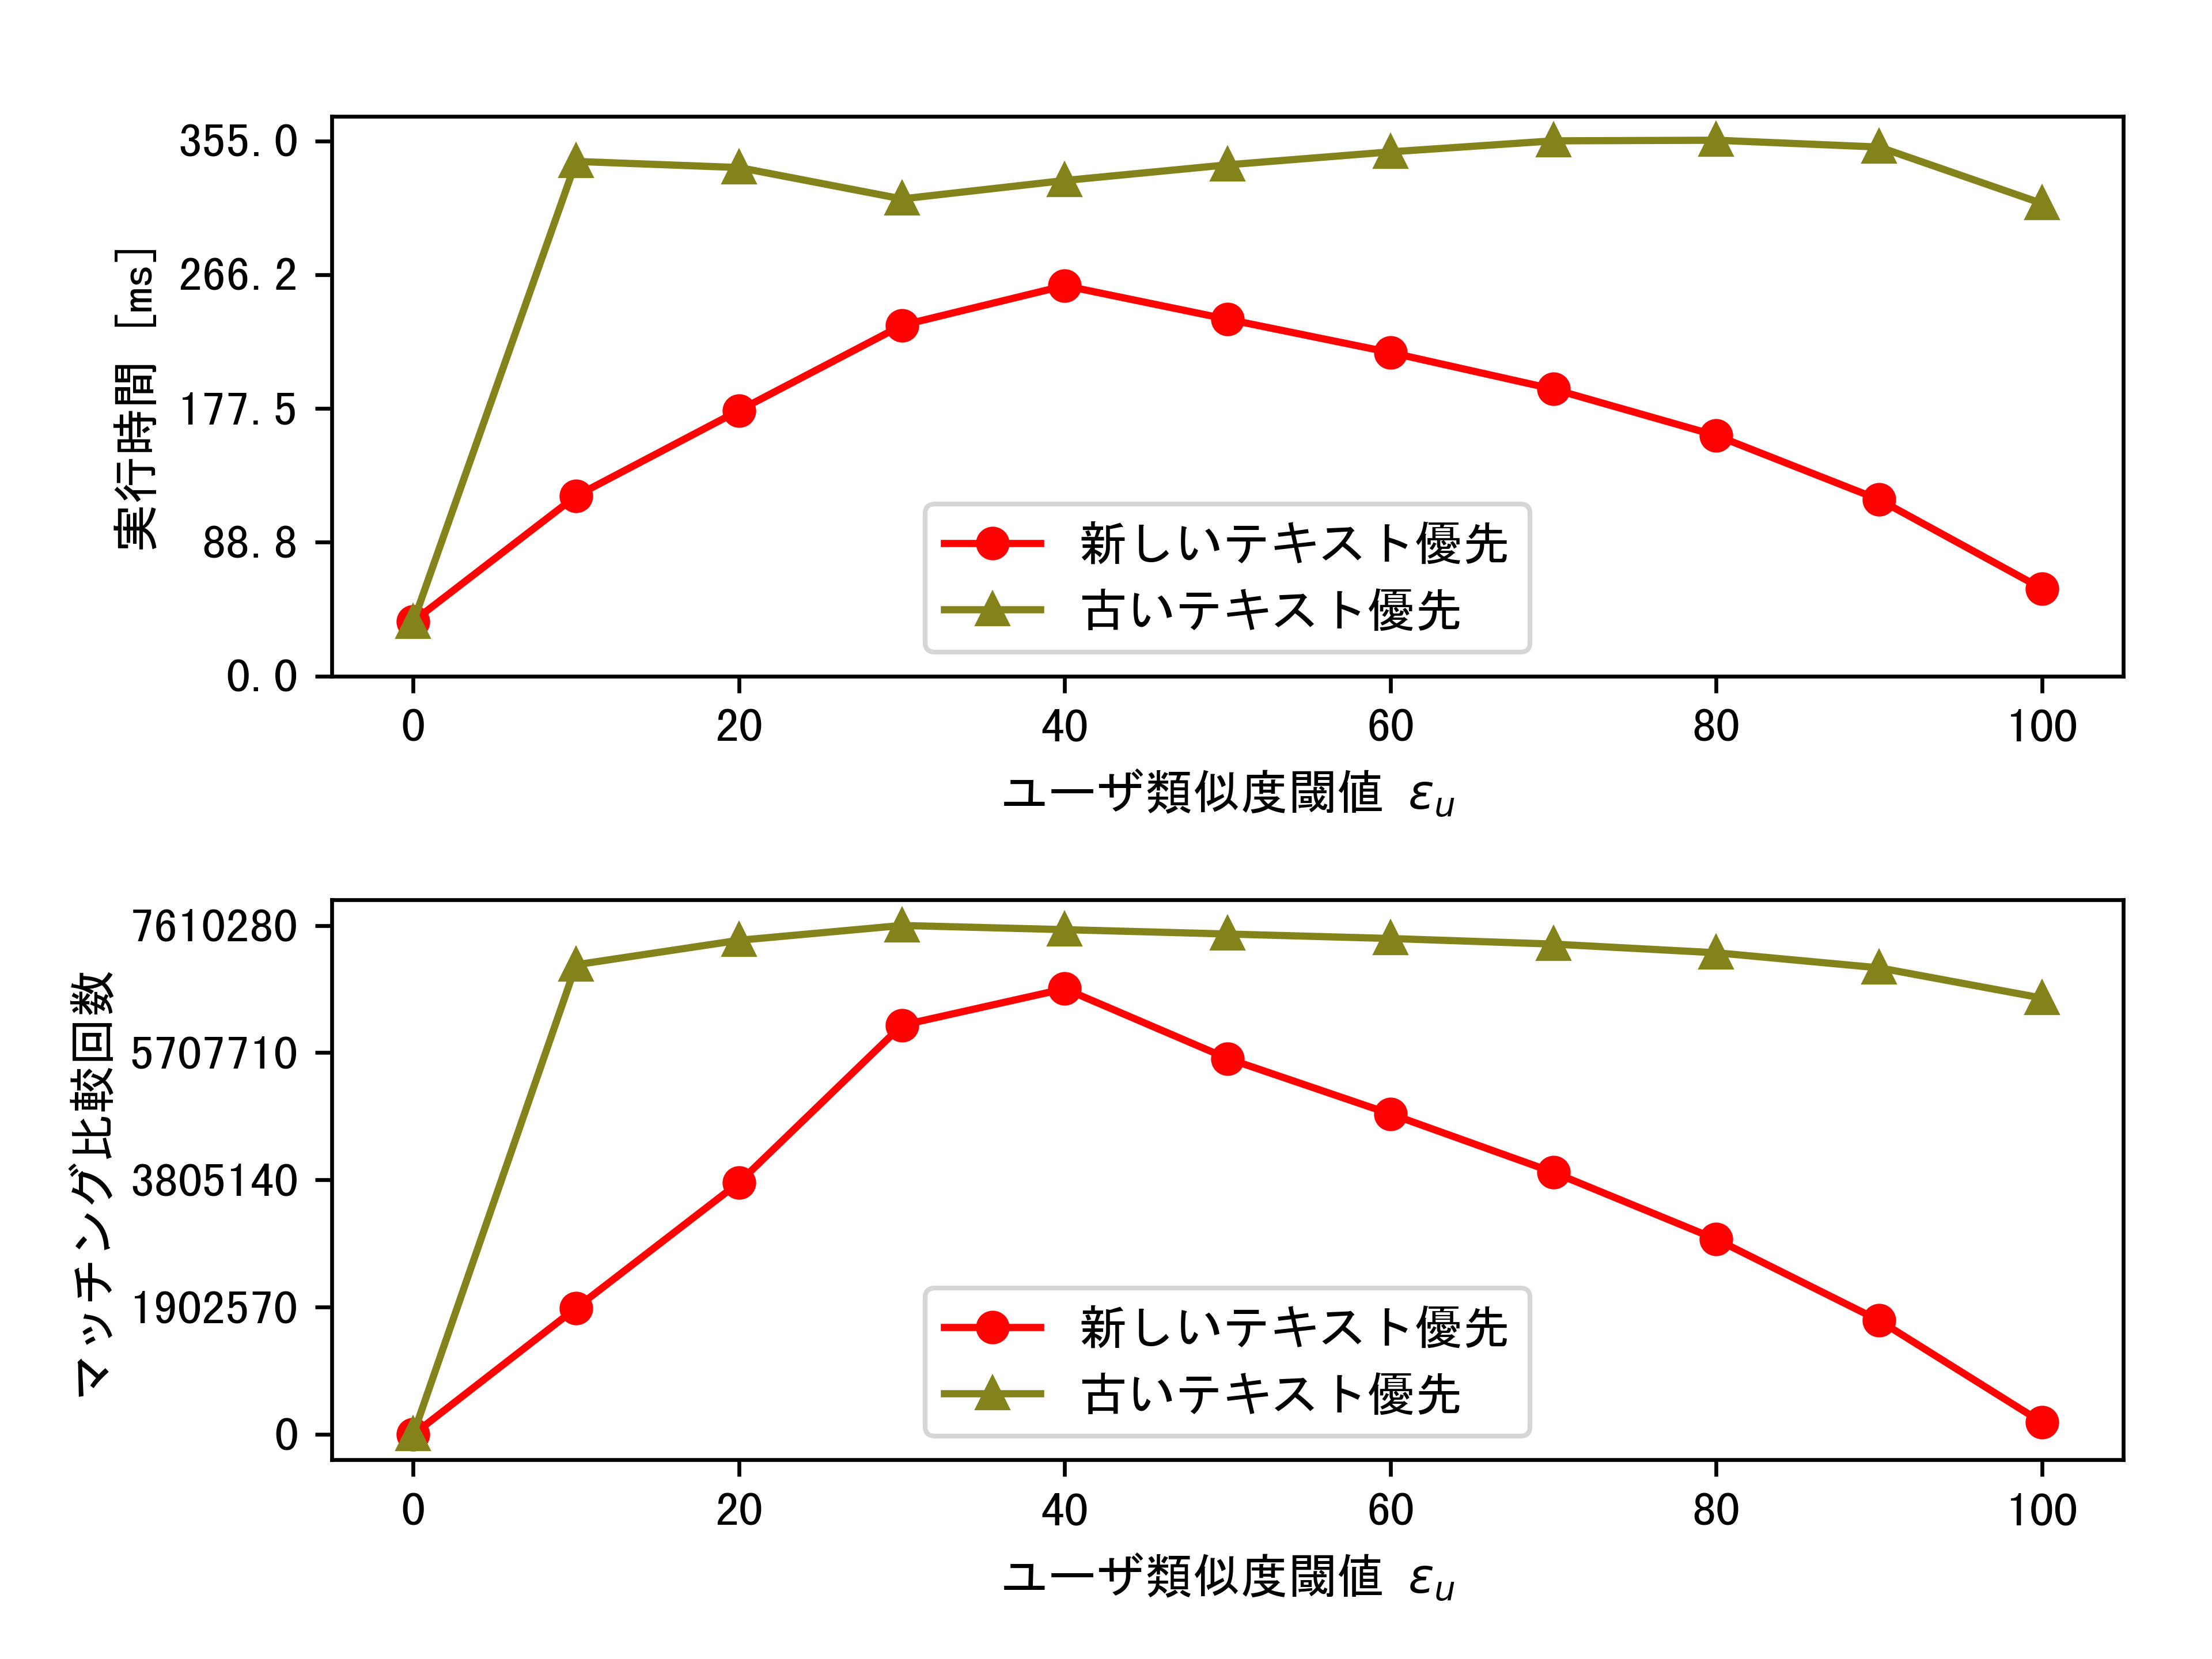
\includegraphics[width=8.3cm]{eimg/exp2_5.png}
    \caption{LE-Qのマッチング順序の優位性評価(人工データセット($p=0.5$))}
    \label{fig:exp2_5}
\end{figure}
\begin{figure}[H]
    \centering
    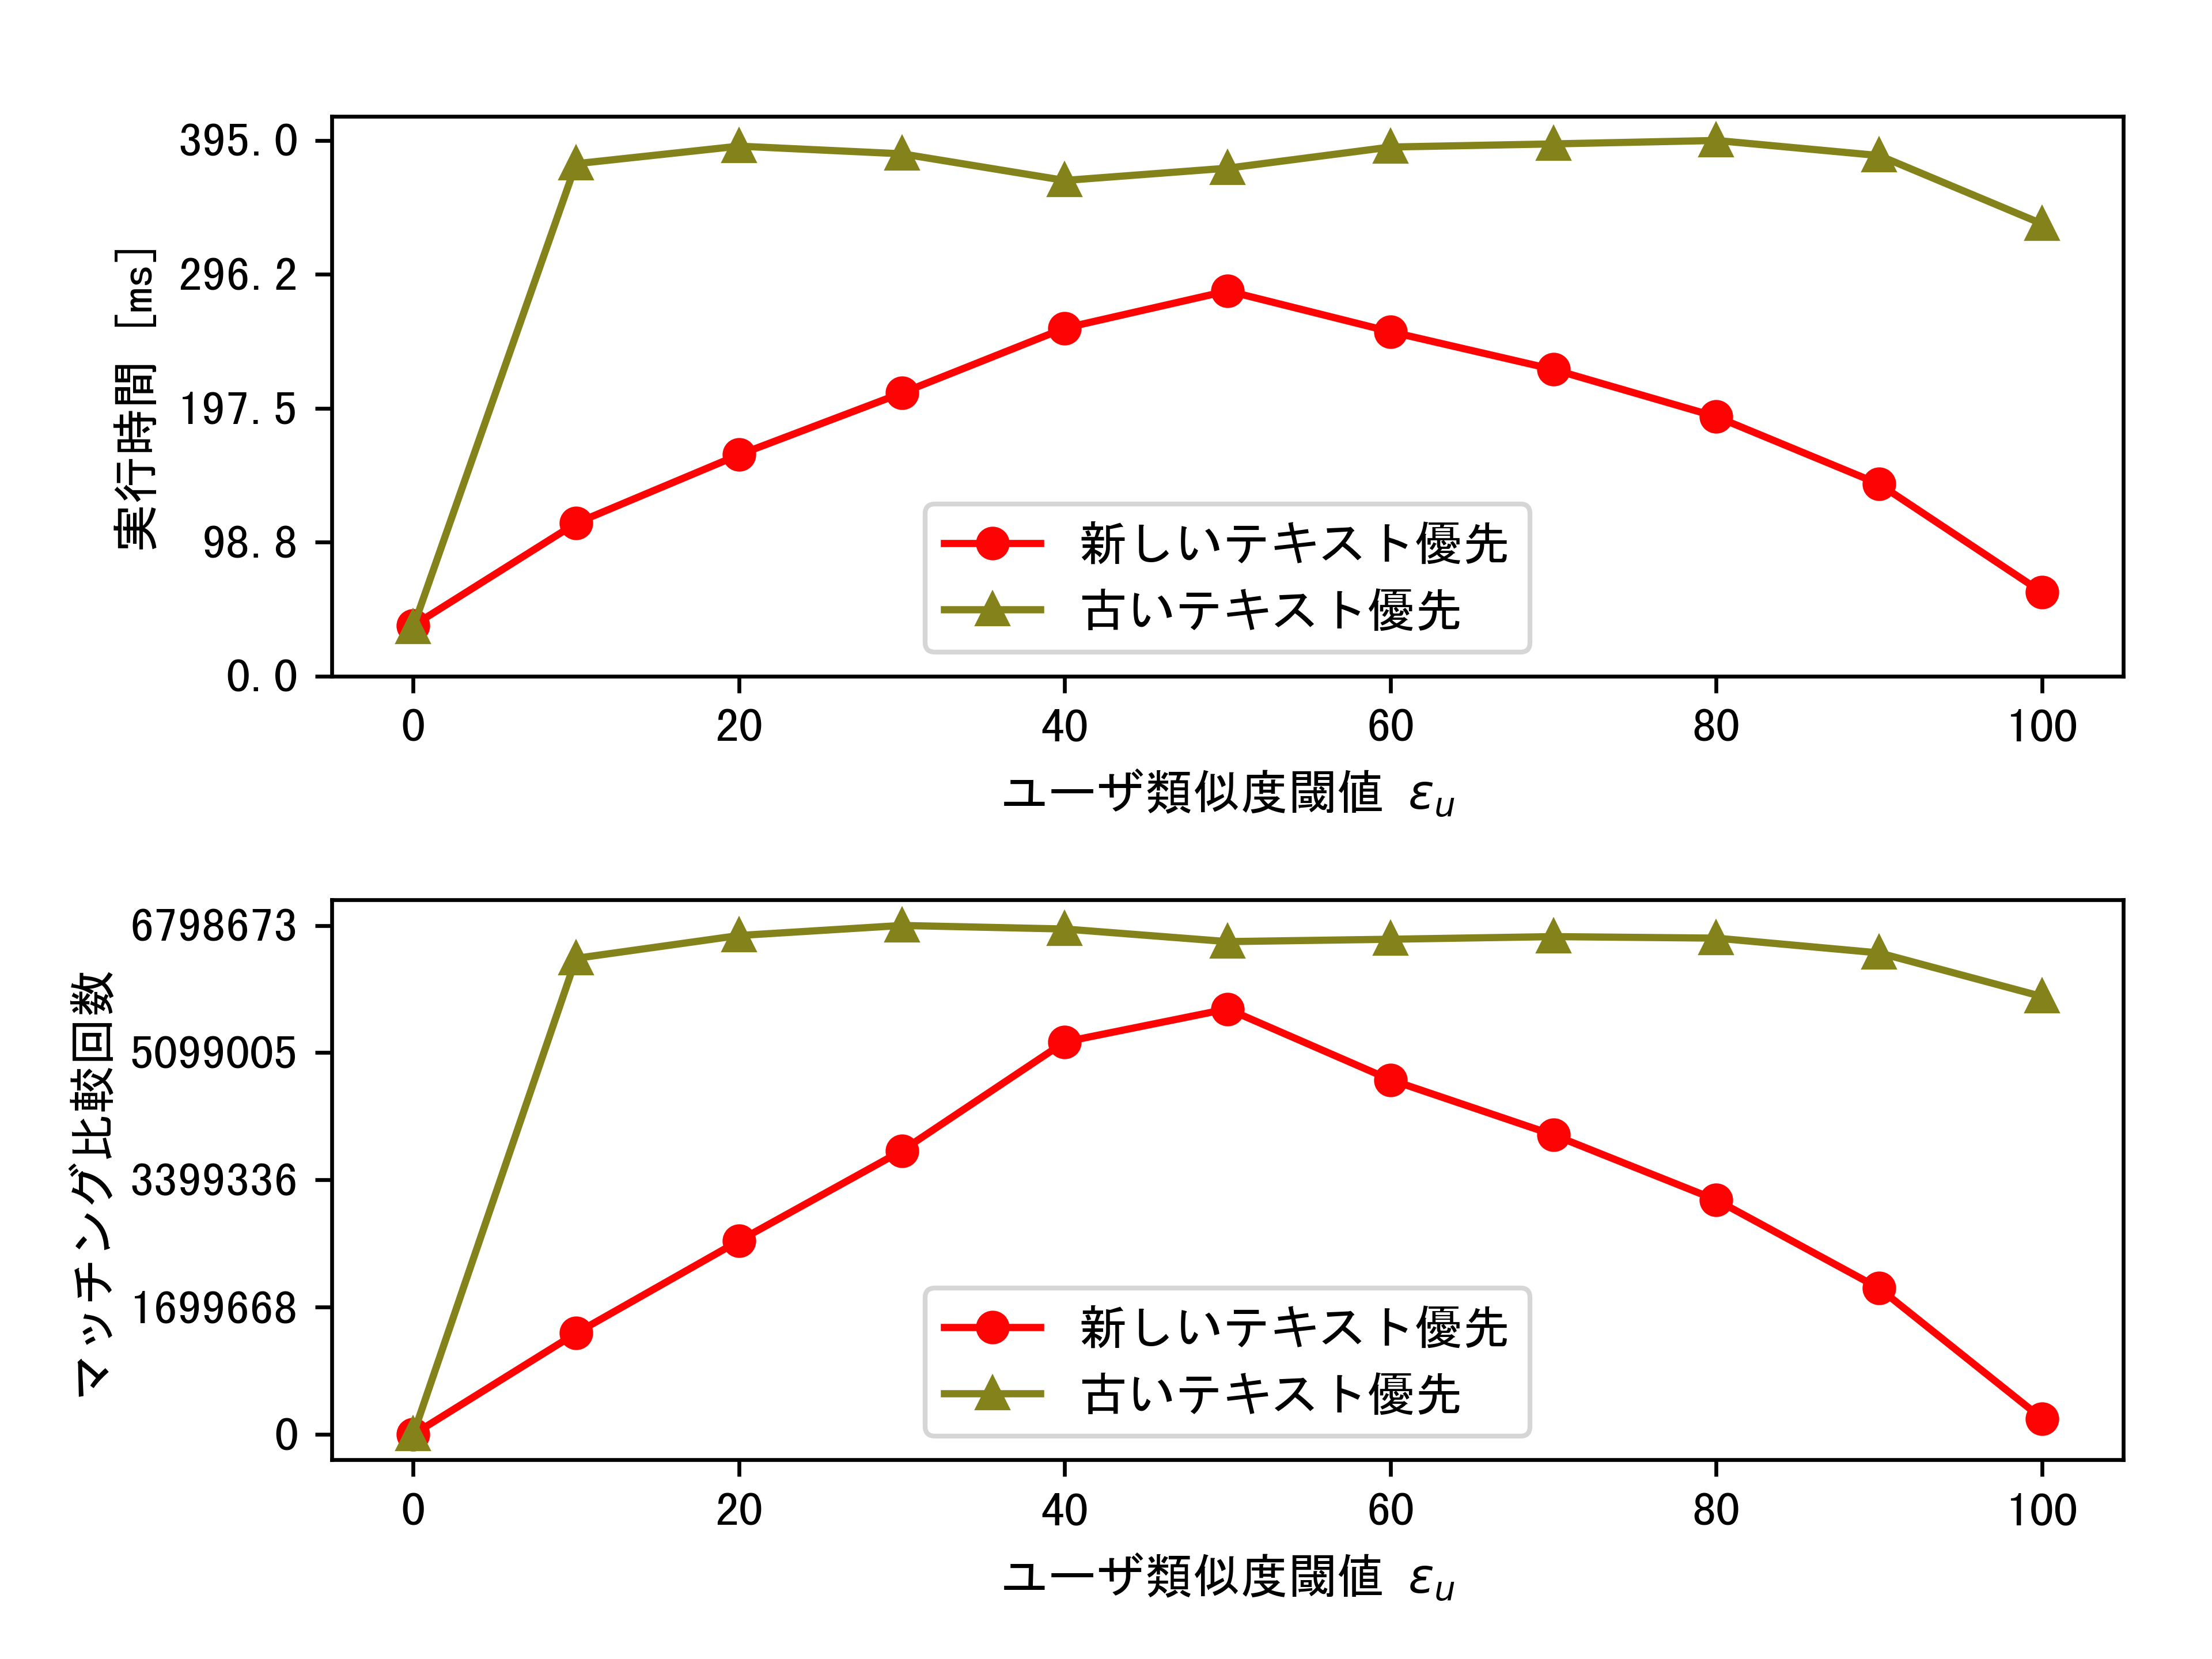
\includegraphics[width=8.3cm]{eimg/exp2_7.png}
    \caption{LE-Qのマッチング順序の優位性評価(人工データセット($p=0.7$))}
    \label{fig:exp2_7}
\end{figure}
\begin{figure}[H]
    \centering
    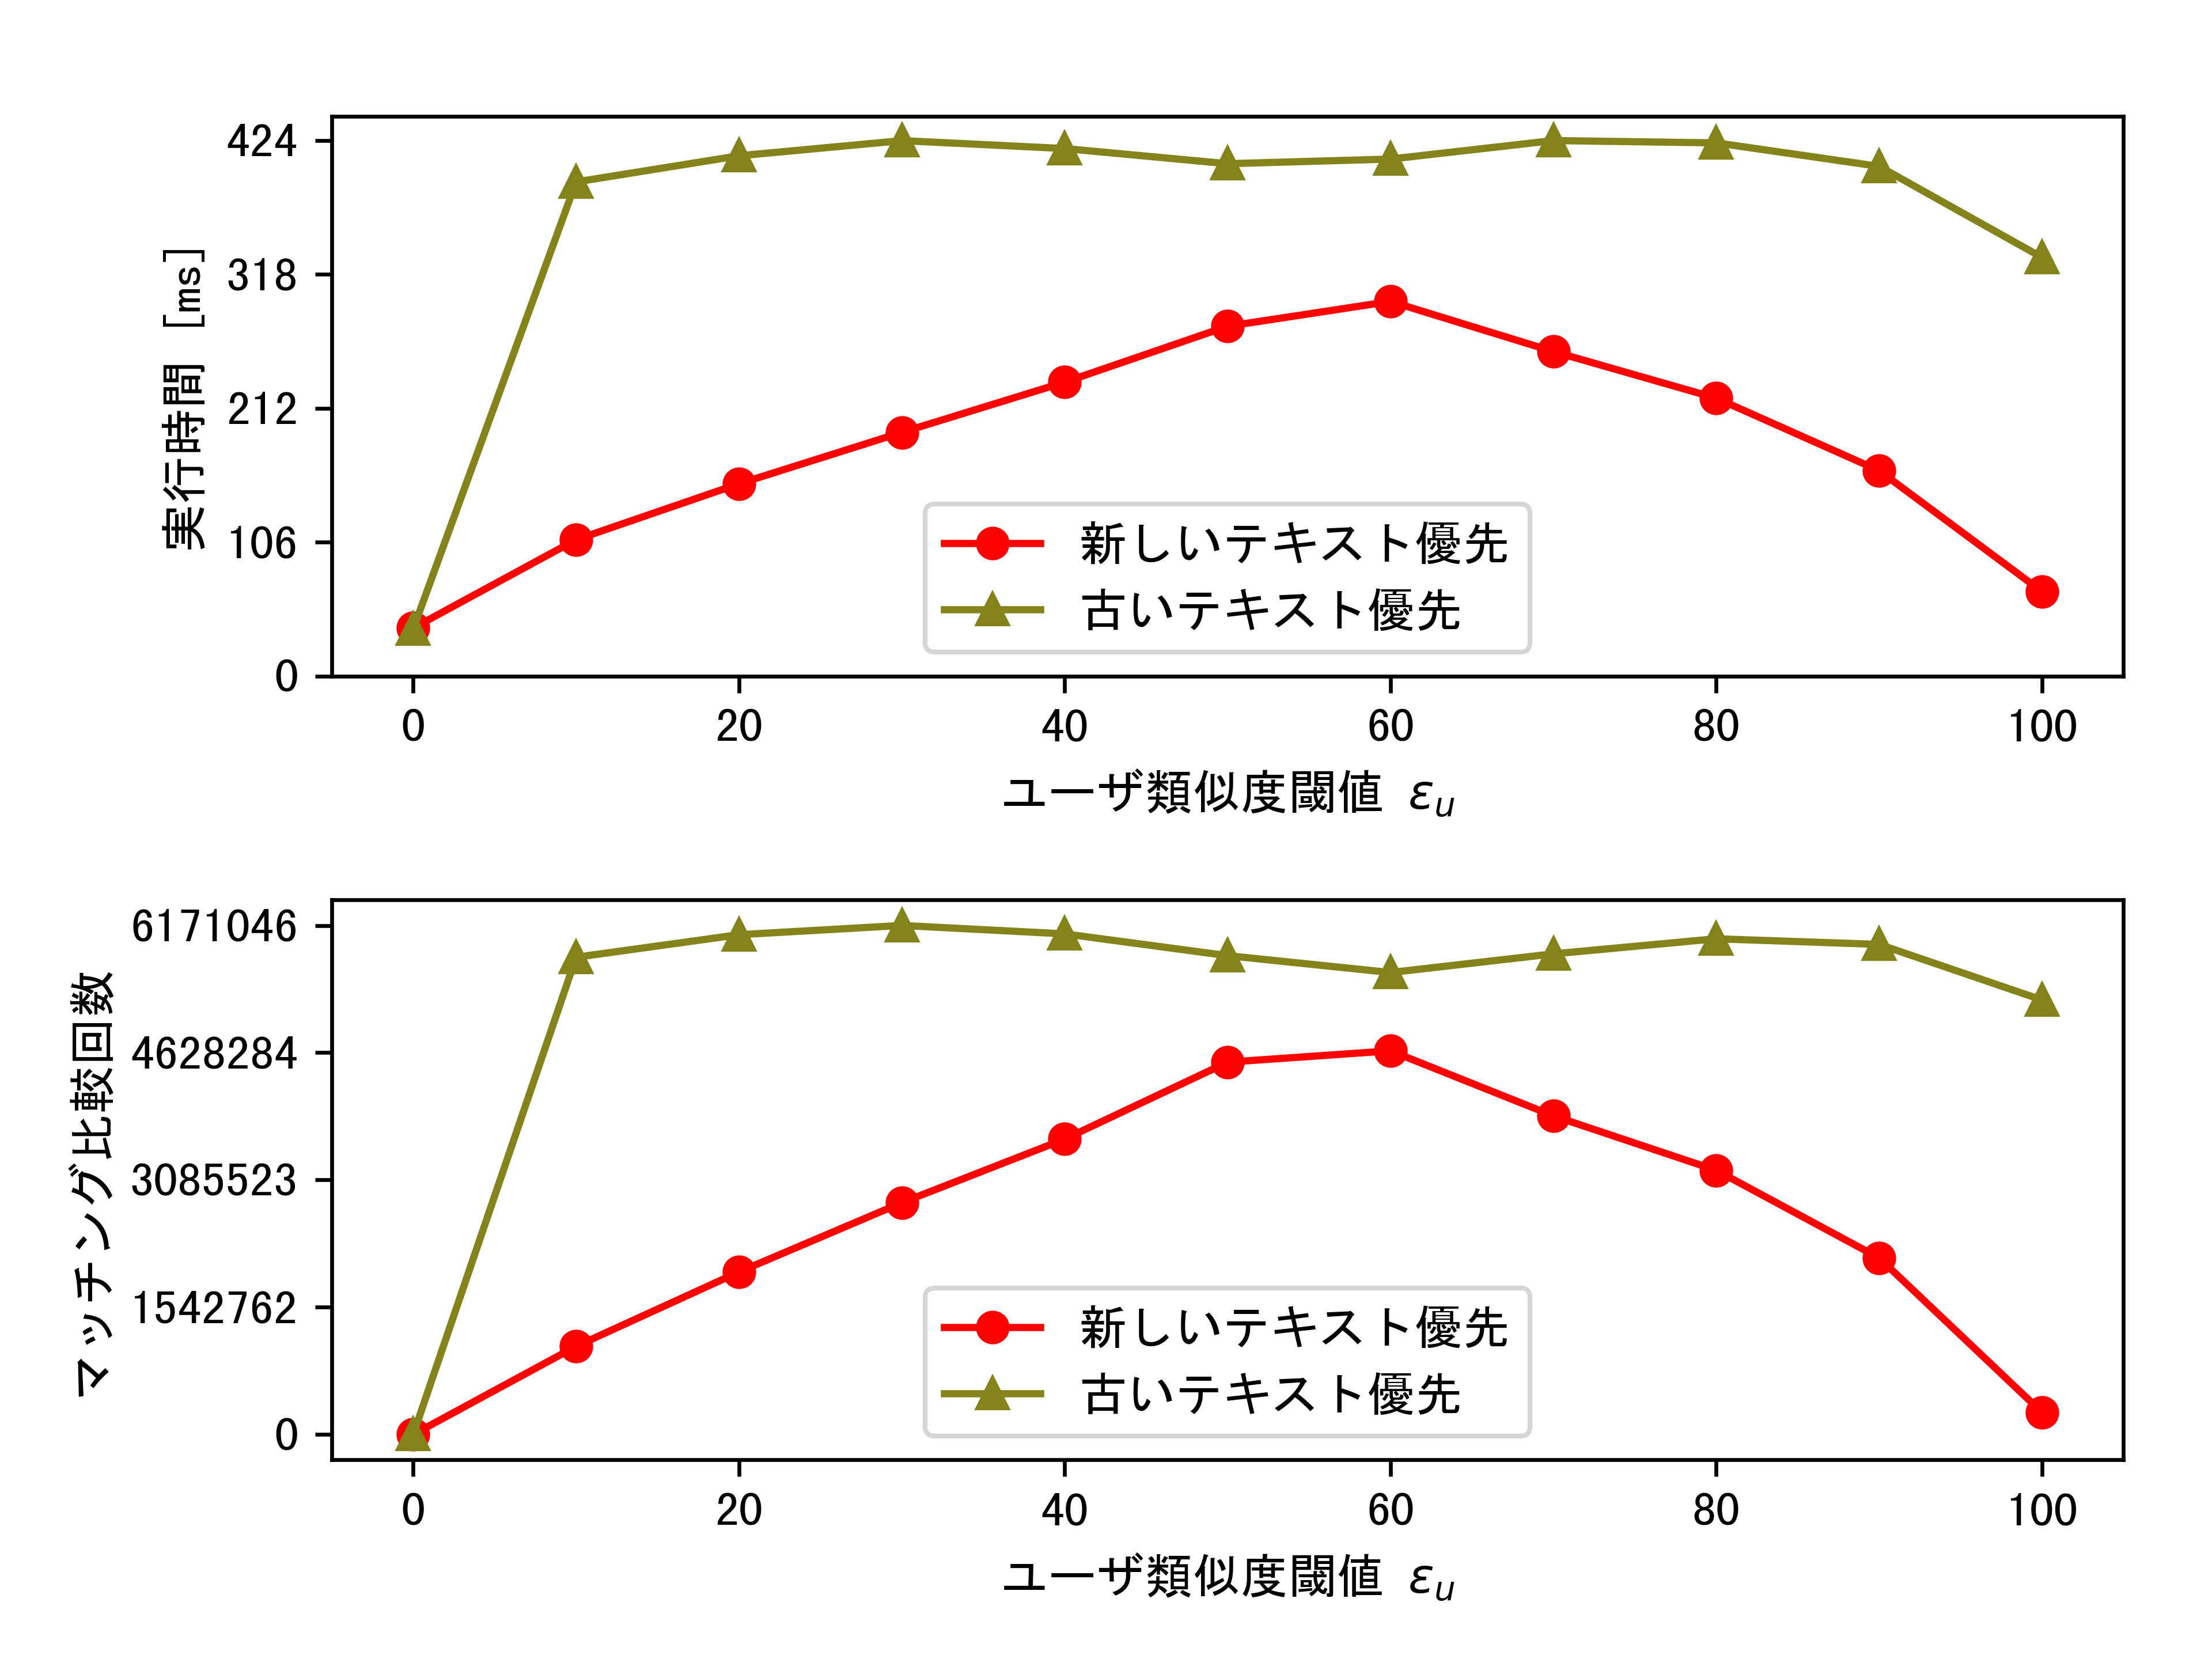
\includegraphics[width=8.3cm]{eimg/exp2_9.png}
    \caption{LE-Qのマッチング順序の優位性評価(人工データセット($p=0.9$))}
    \label{fig:exp2_9}
\end{figure}



\section{ALE-Qの評価}
遅延評価法,LE-Q,LE-Qの改善案であるALE-Qを比較するために,全ユーザの類似性を各時刻すべてにおいて求める実験を行った.$\epsilon_r$を40,$\epsilon_m$を5としたときの人工データセットにおける実験結果を図\ref{fig:exp3}に示した.
結果より,ALE-Qの方がLE-Qより実行時間が短くなっていることがわかる.これはある程度少ない数のテキストのマッチング判定を行わなくてはいけないとき,転置インデクスを用いたマッチングに変更することで共通の単語を1つも持たないテキストへのマッチングを避けることができたからであると考える.さらにかなり少ない数のテキストのマッチング判定を行わなくてはいけないとき,転置インデクスを用いないマッチング方法にすることでマッチング判定を行うテキストの個数を減らすことが出来たからであると考える.

\begin{figure}[H]
    \centering
    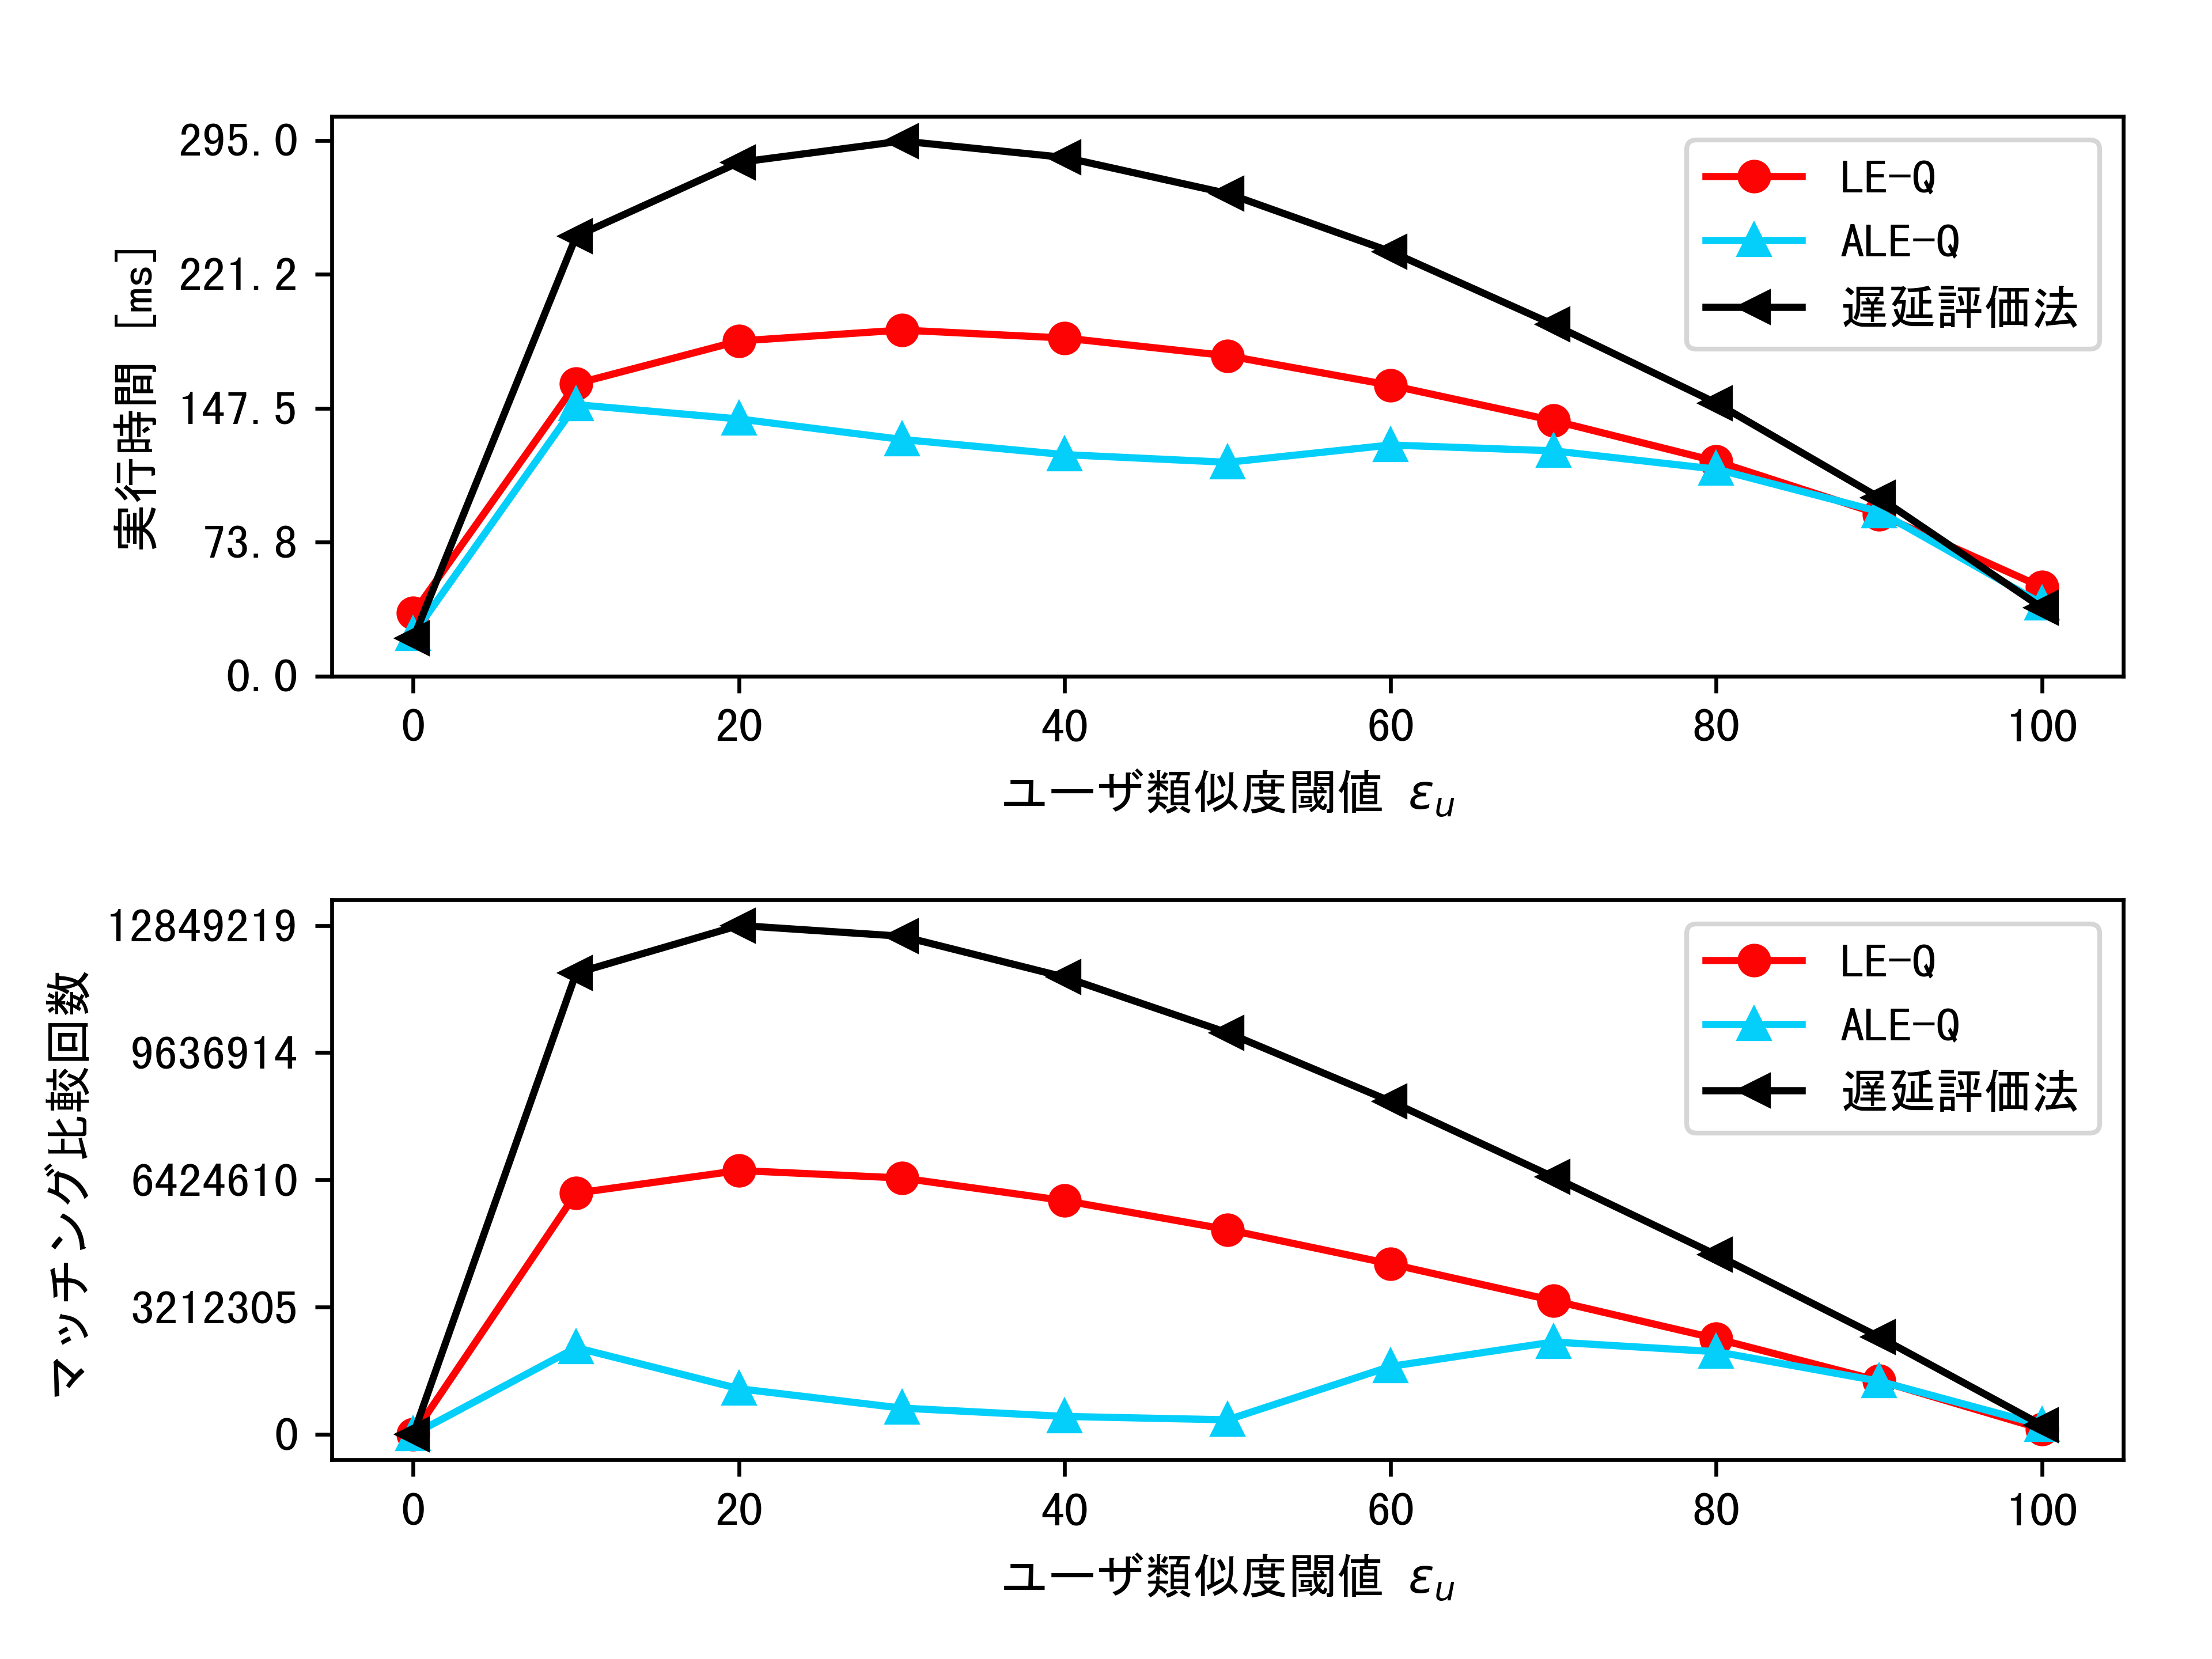
\includegraphics[width=8.3cm]{eimg/exp3.png}
    \caption{ALE-Qの性能比較(人工データセット($p=0.96^{(i-1)}$))}
    \label{fig:exp3}
\end{figure}
$\epsilon_r$を55,$\epsilon_m$を5としたCoPhIRデータセットにおける実験結果を図\ref{fig:exp3_c}に示した.人工データの実験の図\ref{fig:exp3}と同様にALE-Qの方がLE-Qより早くなっていることがわかる.
%図\ref{fig:exp3_c}は人工データによる実験と同様の結果を示し,ALE-Qは本研究で最も効率的なアルゴリズムであるといえる.
\begin{figure}[H]
    \centering
    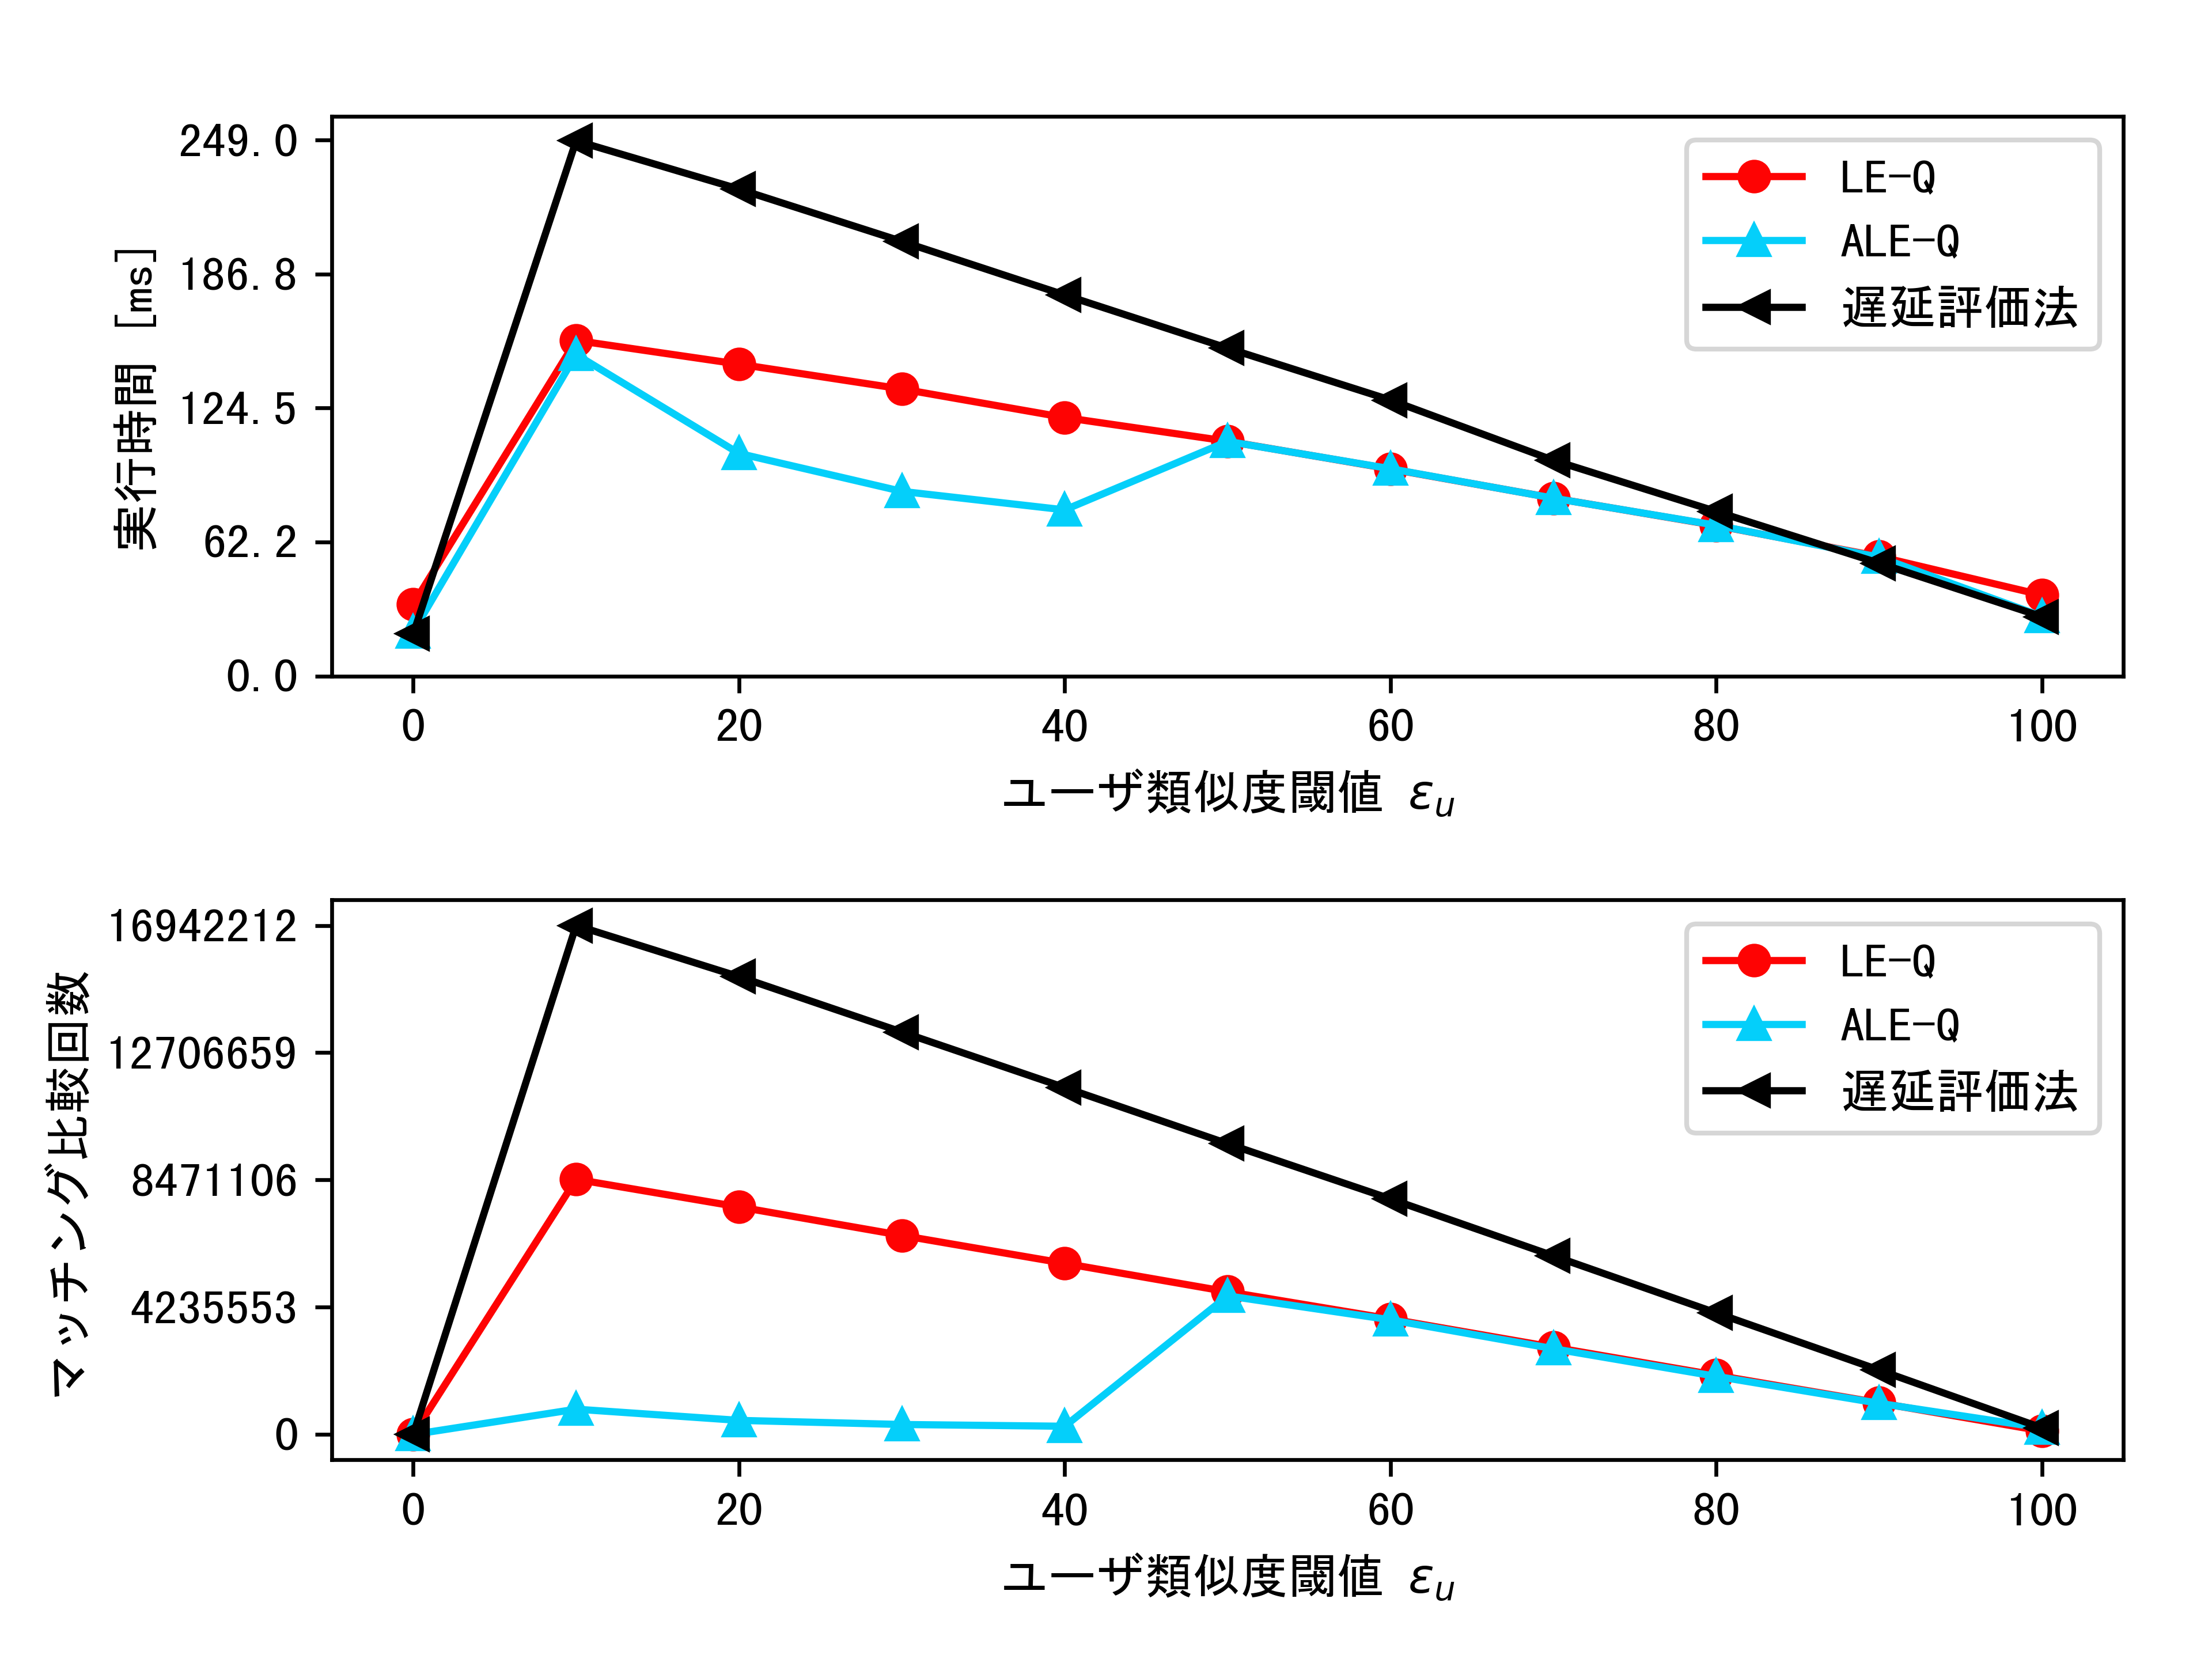
\includegraphics[width=8.3cm]{eimg/exp3_c.png}
    \caption{ALE-Qの性能比較(CoPhIRデータセット)}
    \label{fig:exp3_c}
\end{figure}

$\epsilon_r$を40,$\epsilon_m$を5としたときの人工データセットにおける$p$を固定した場合の実験結果を図\ref{fig:exp3_1},図\ref{fig:exp3_3},図\ref{fig:exp3_5},図\ref{fig:exp3_7},図\ref{fig:exp3_9}に示した.
%\ref{exp1}節ではクエリユーザに対するデータベースユーザの類似度が大きいとき遅延評価法よりLE-Qの方が実行時間が多くかかっていたが,今回の実験で改善案のALE-Qは類似度が大きい場合でも遅延評価法以下の実行時間で処理することが出来ることを示せた.
閾値$\epsilon_r$,$\epsilon_m$を用いた転置インデクス利用の切り替えを適応的に行った結果,マッチング比較回数を削減することに繋がり,$p$の値によらずLE-QよりもALE-Qの方が実行時間が短くなるという結果が示された.

\begin{figure}[H]
    \centering
    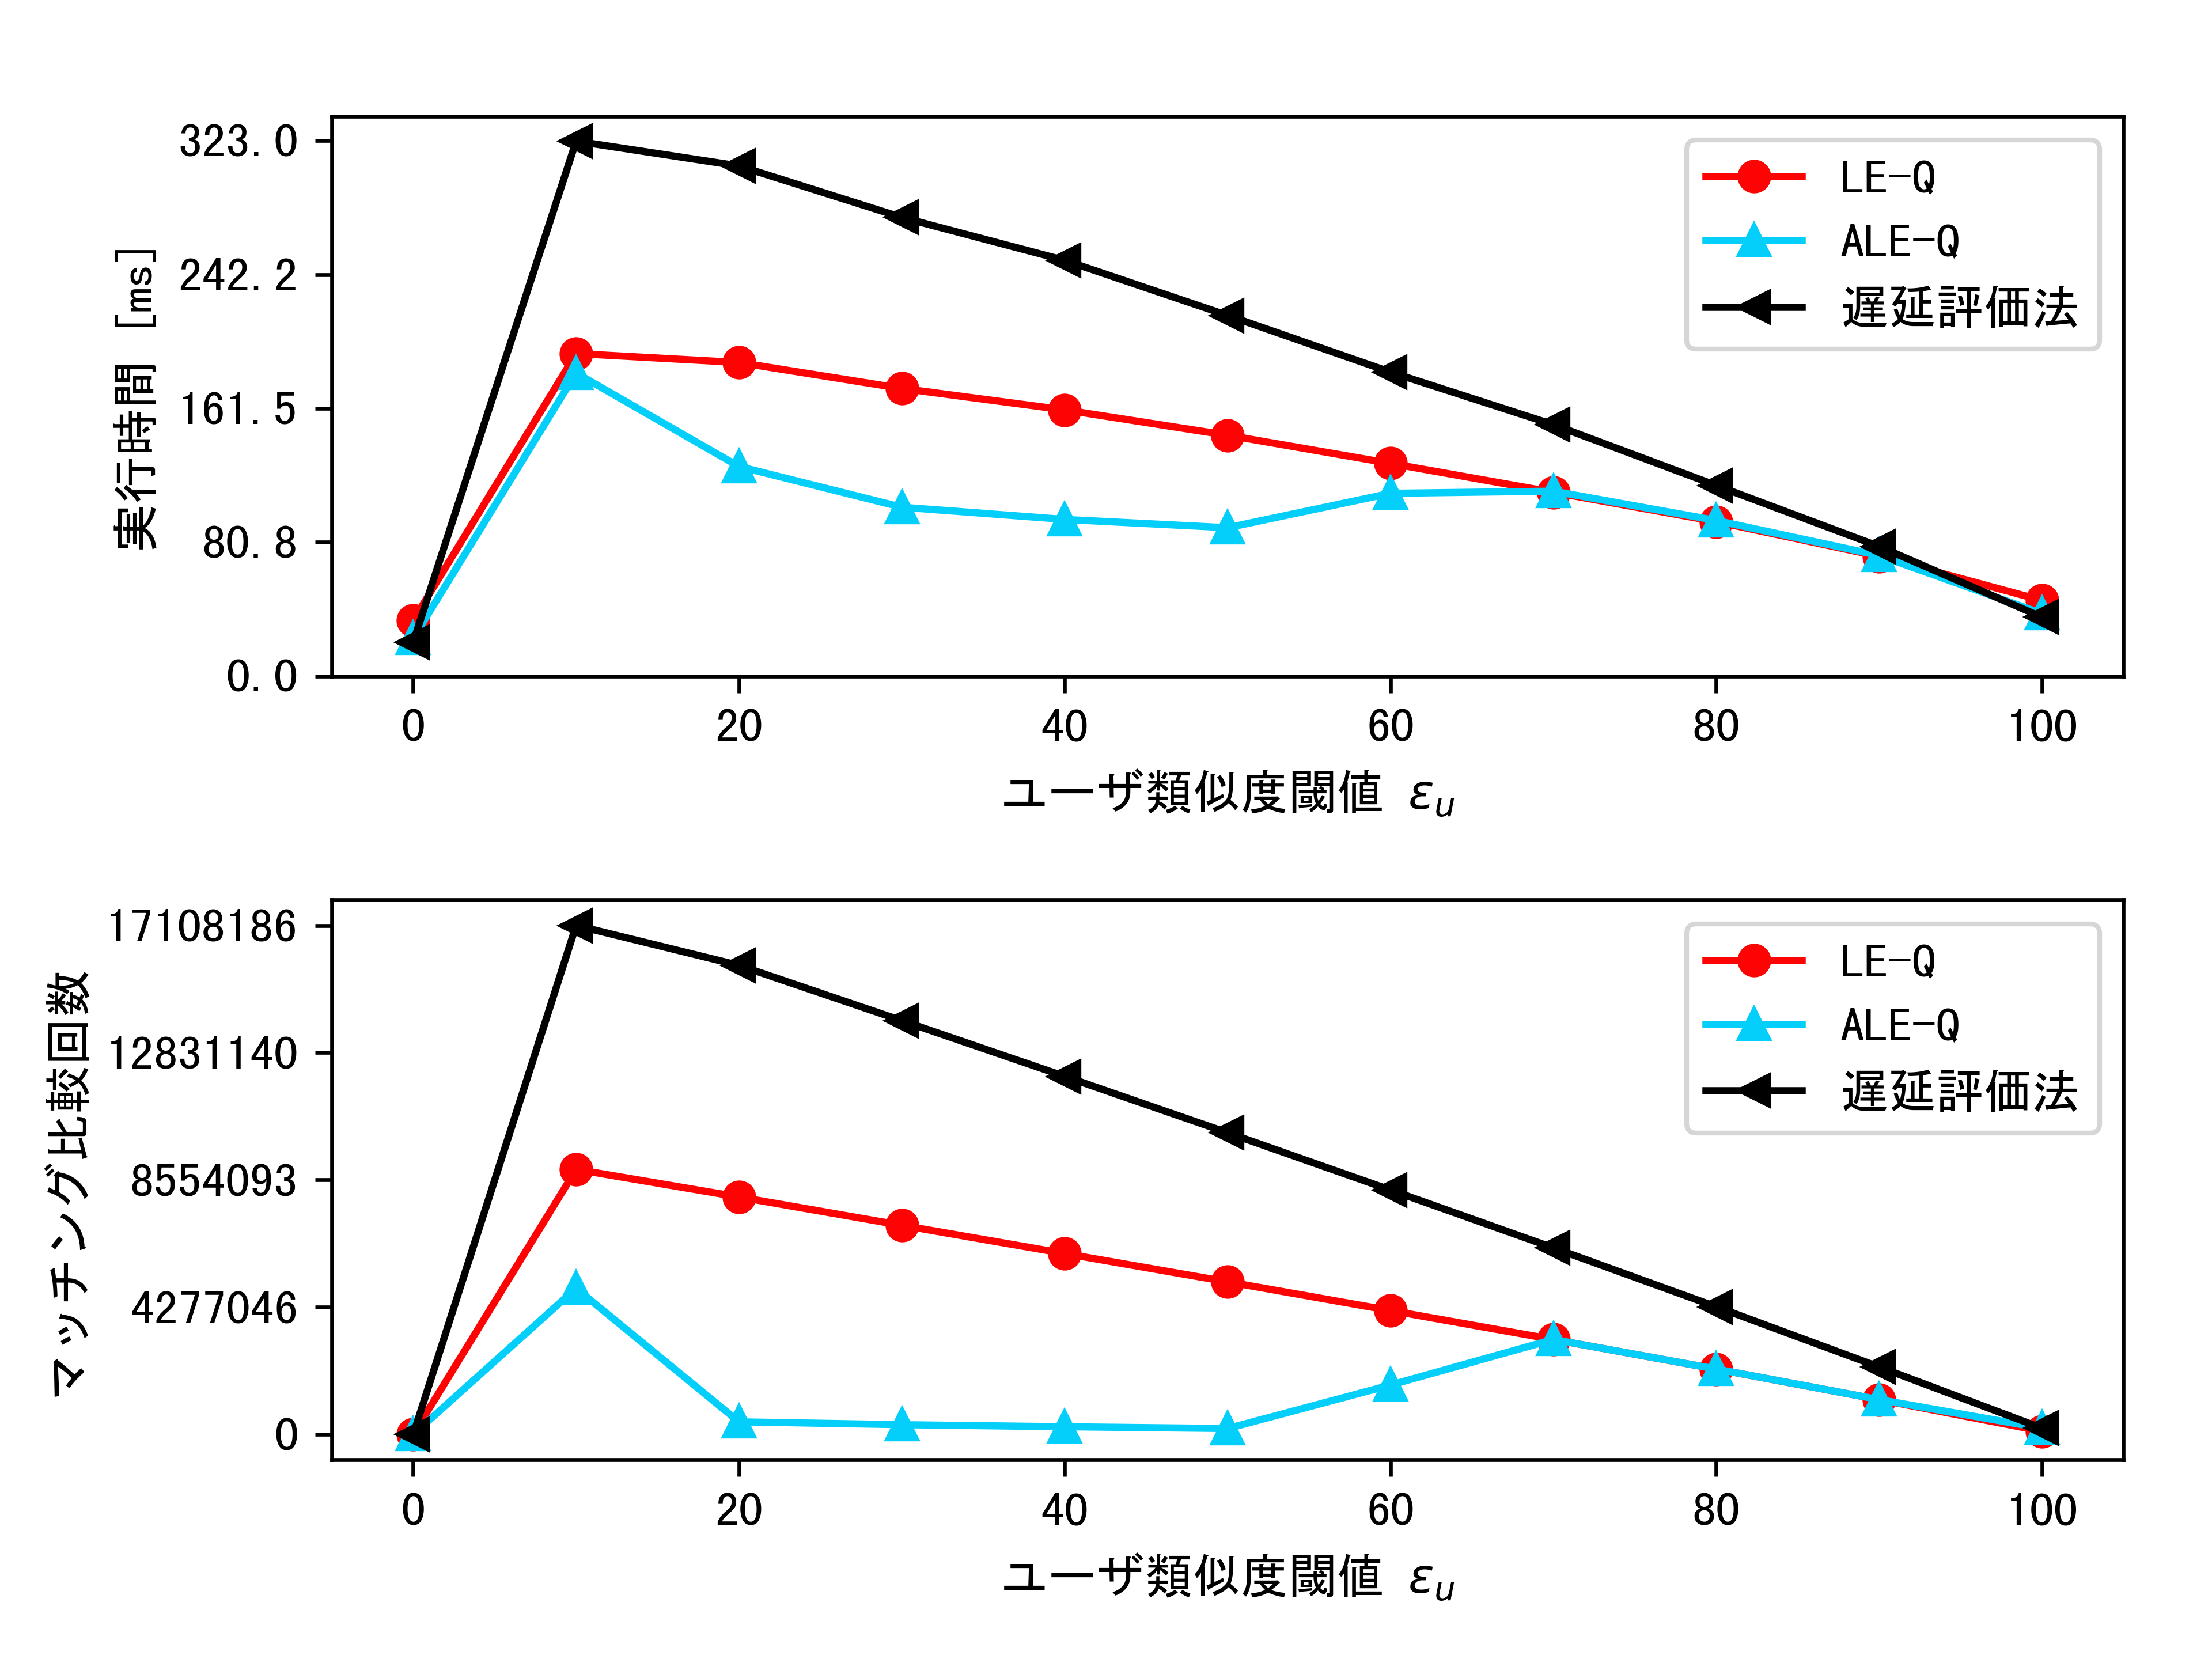
\includegraphics[width=8.3cm]{eimg/exp3_1.png}
    \caption{ALE-Qの性能比較(人工データセット($p=0.1$))}
    \label{fig:exp3_1}
\end{figure}
\begin{figure}[H]
    \centering
    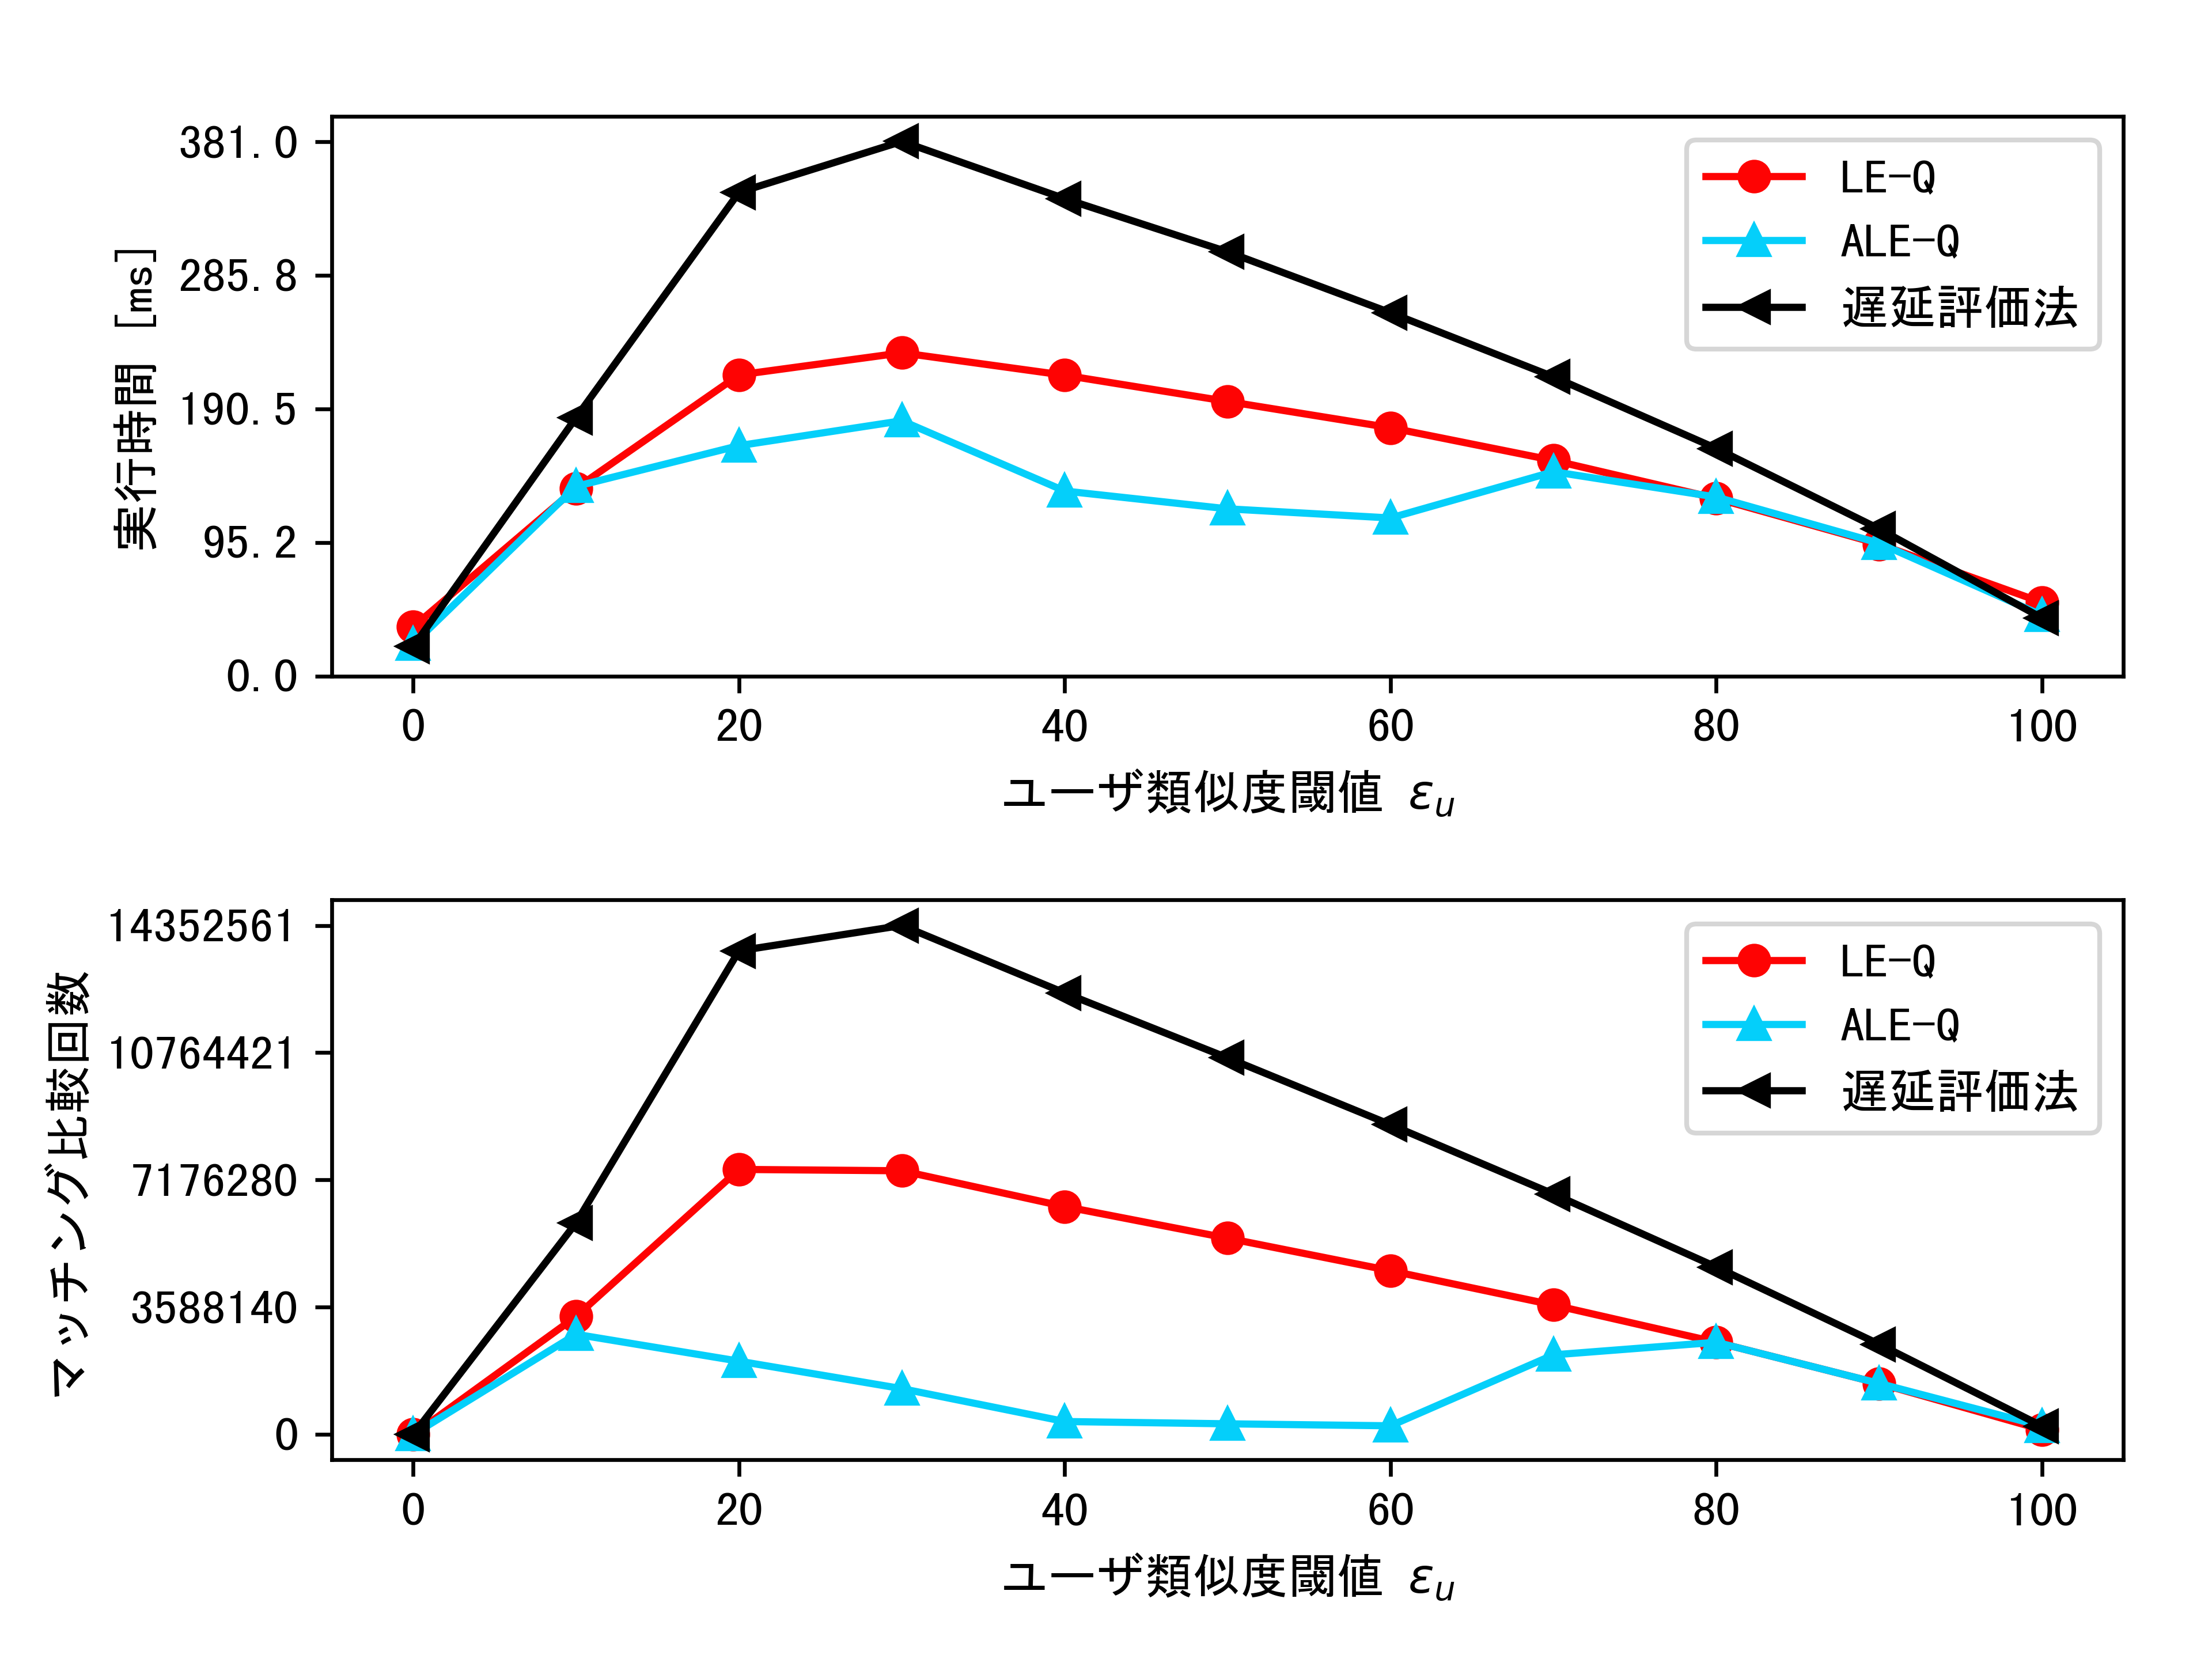
\includegraphics[width=8.3cm]{eimg/exp3_3.png}
    \caption{ALE-Qの性能比較(人工データセット($p=0.3$))}
    \label{fig:exp3_3}
\end{figure}
\begin{figure}[H]
    \centering
    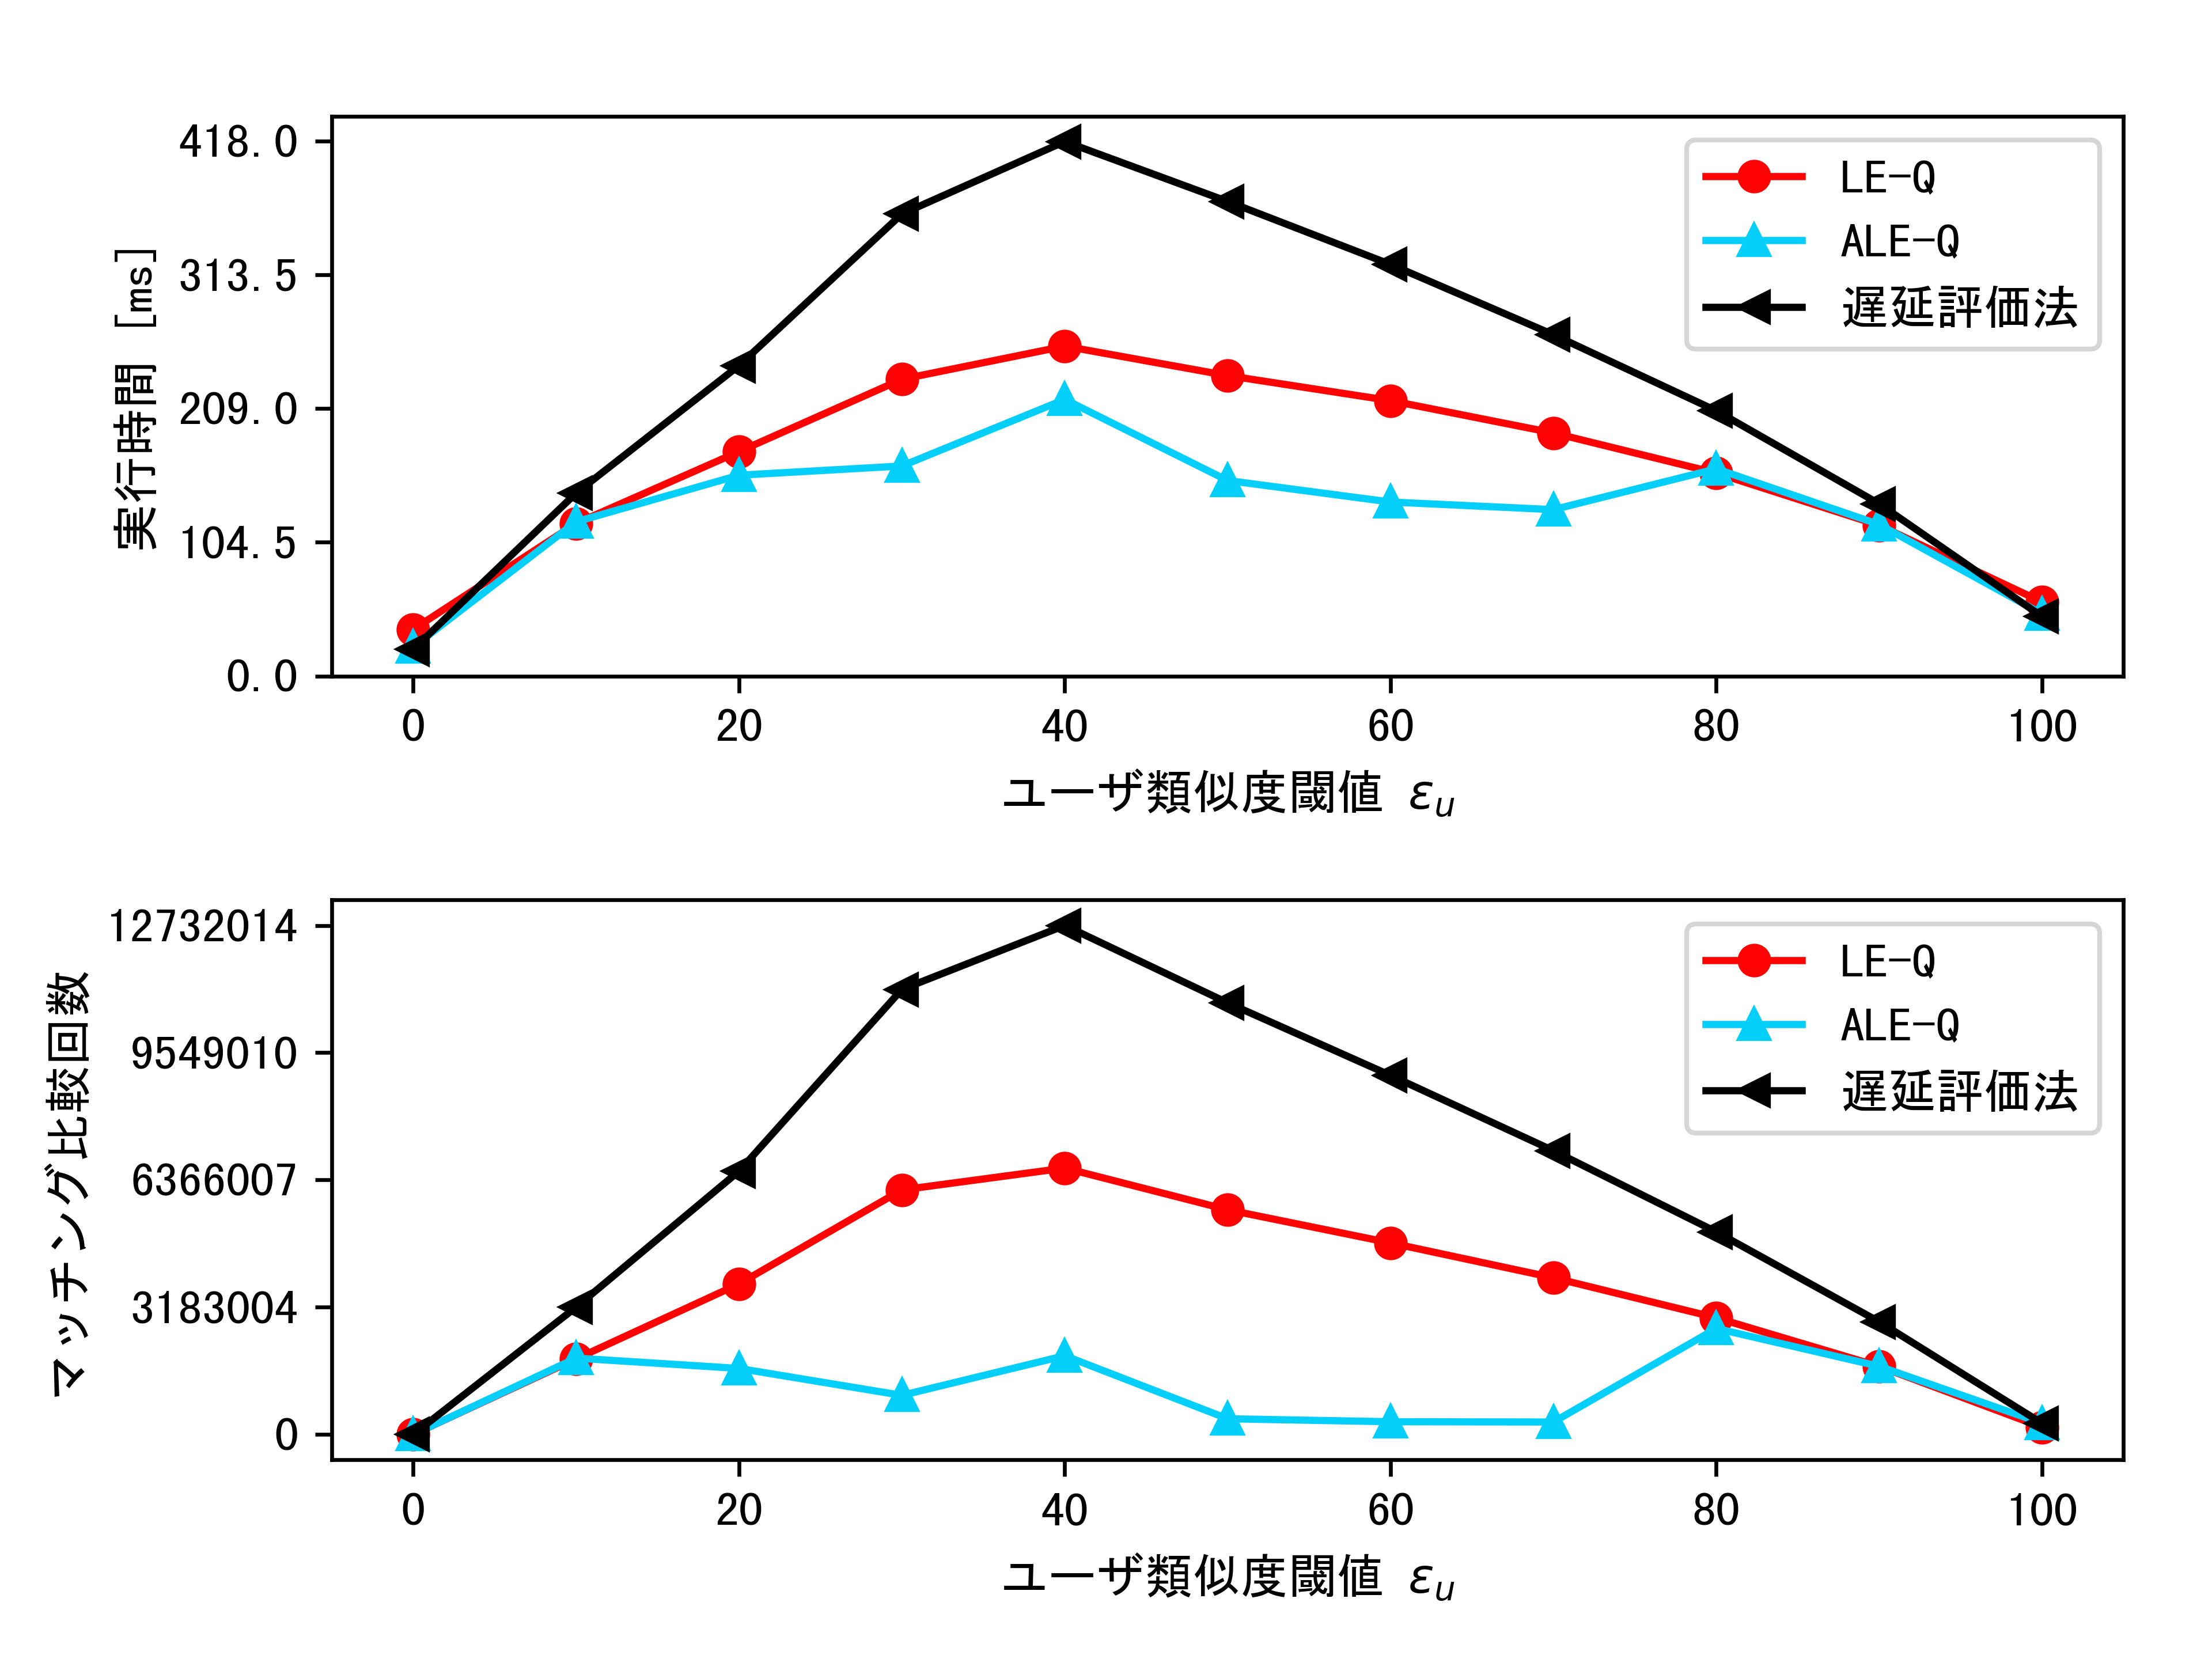
\includegraphics[width=8.3cm]{eimg/exp3_5.png}
    \caption{ALE-Qの性能比較(人工データセット($p=0.5$))}
    \label{fig:exp3_5}
\end{figure}
\begin{figure}[H]
    \centering
    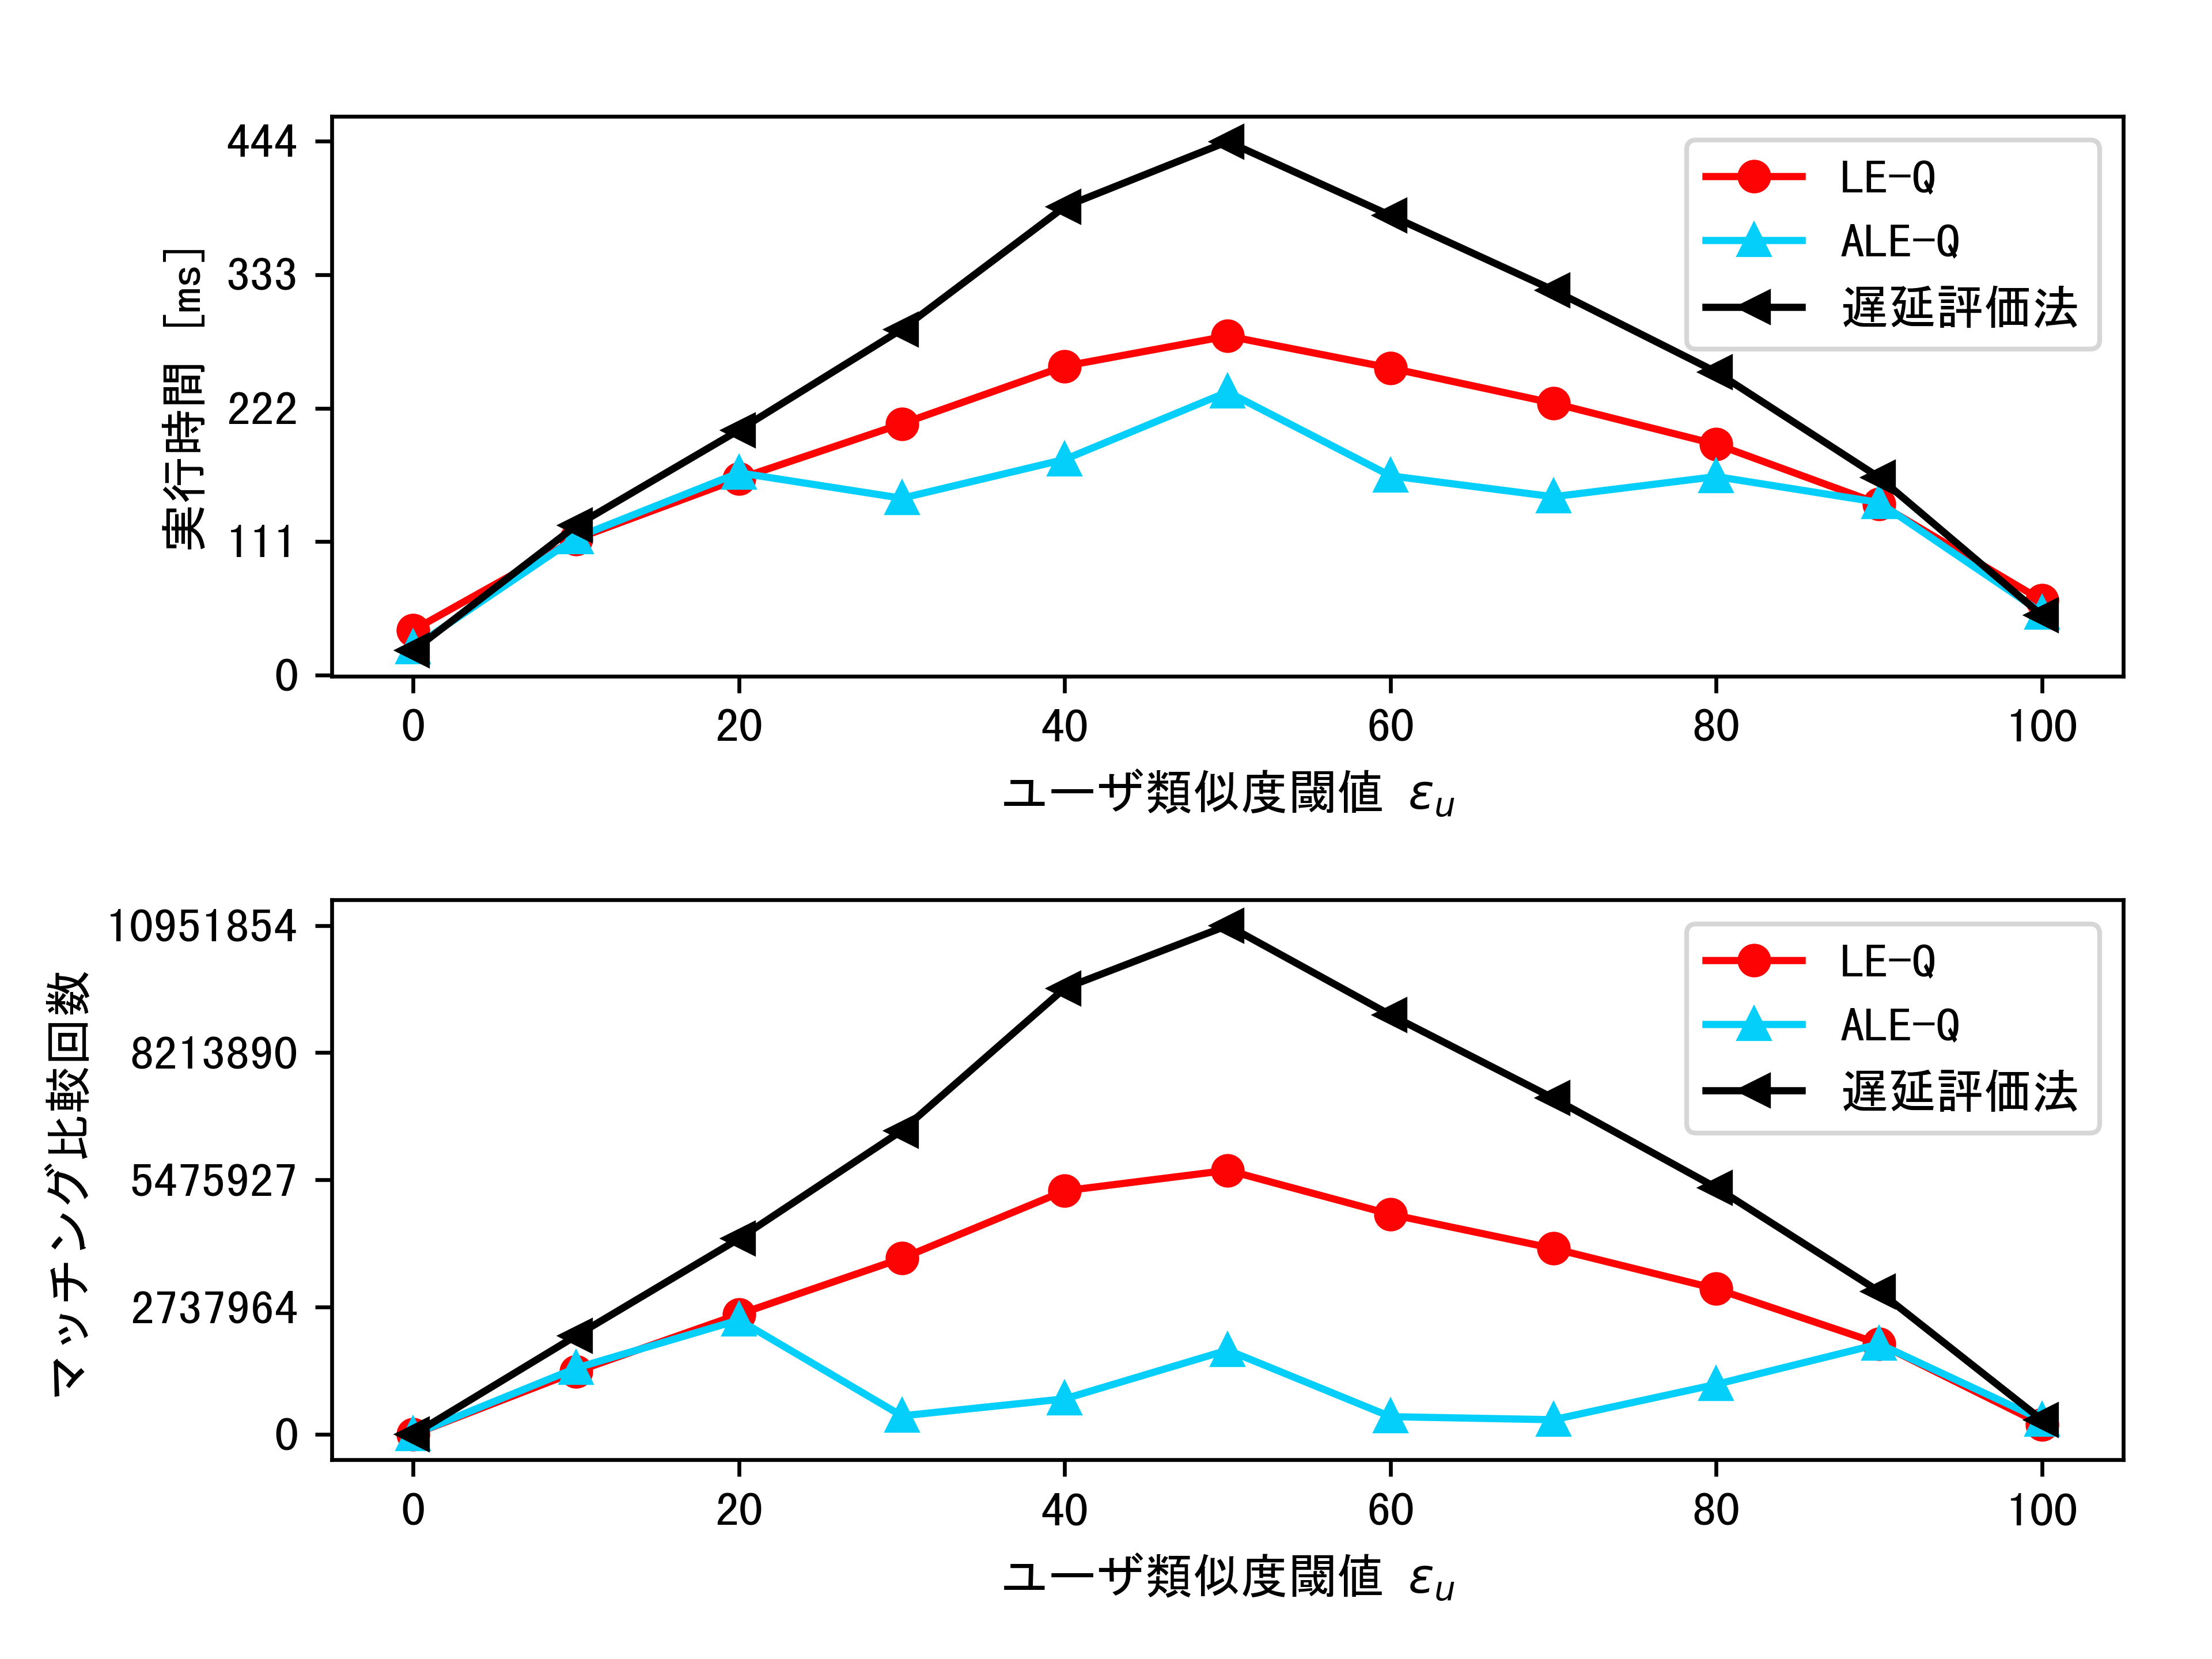
\includegraphics[width=8.3cm]{eimg/exp3_7.png}
    \caption{ALE-Qの性能比較(人工データセット($p=0.7$))}
    \label{fig:exp3_7}
\end{figure}
\begin{figure}[H]
    \centering
    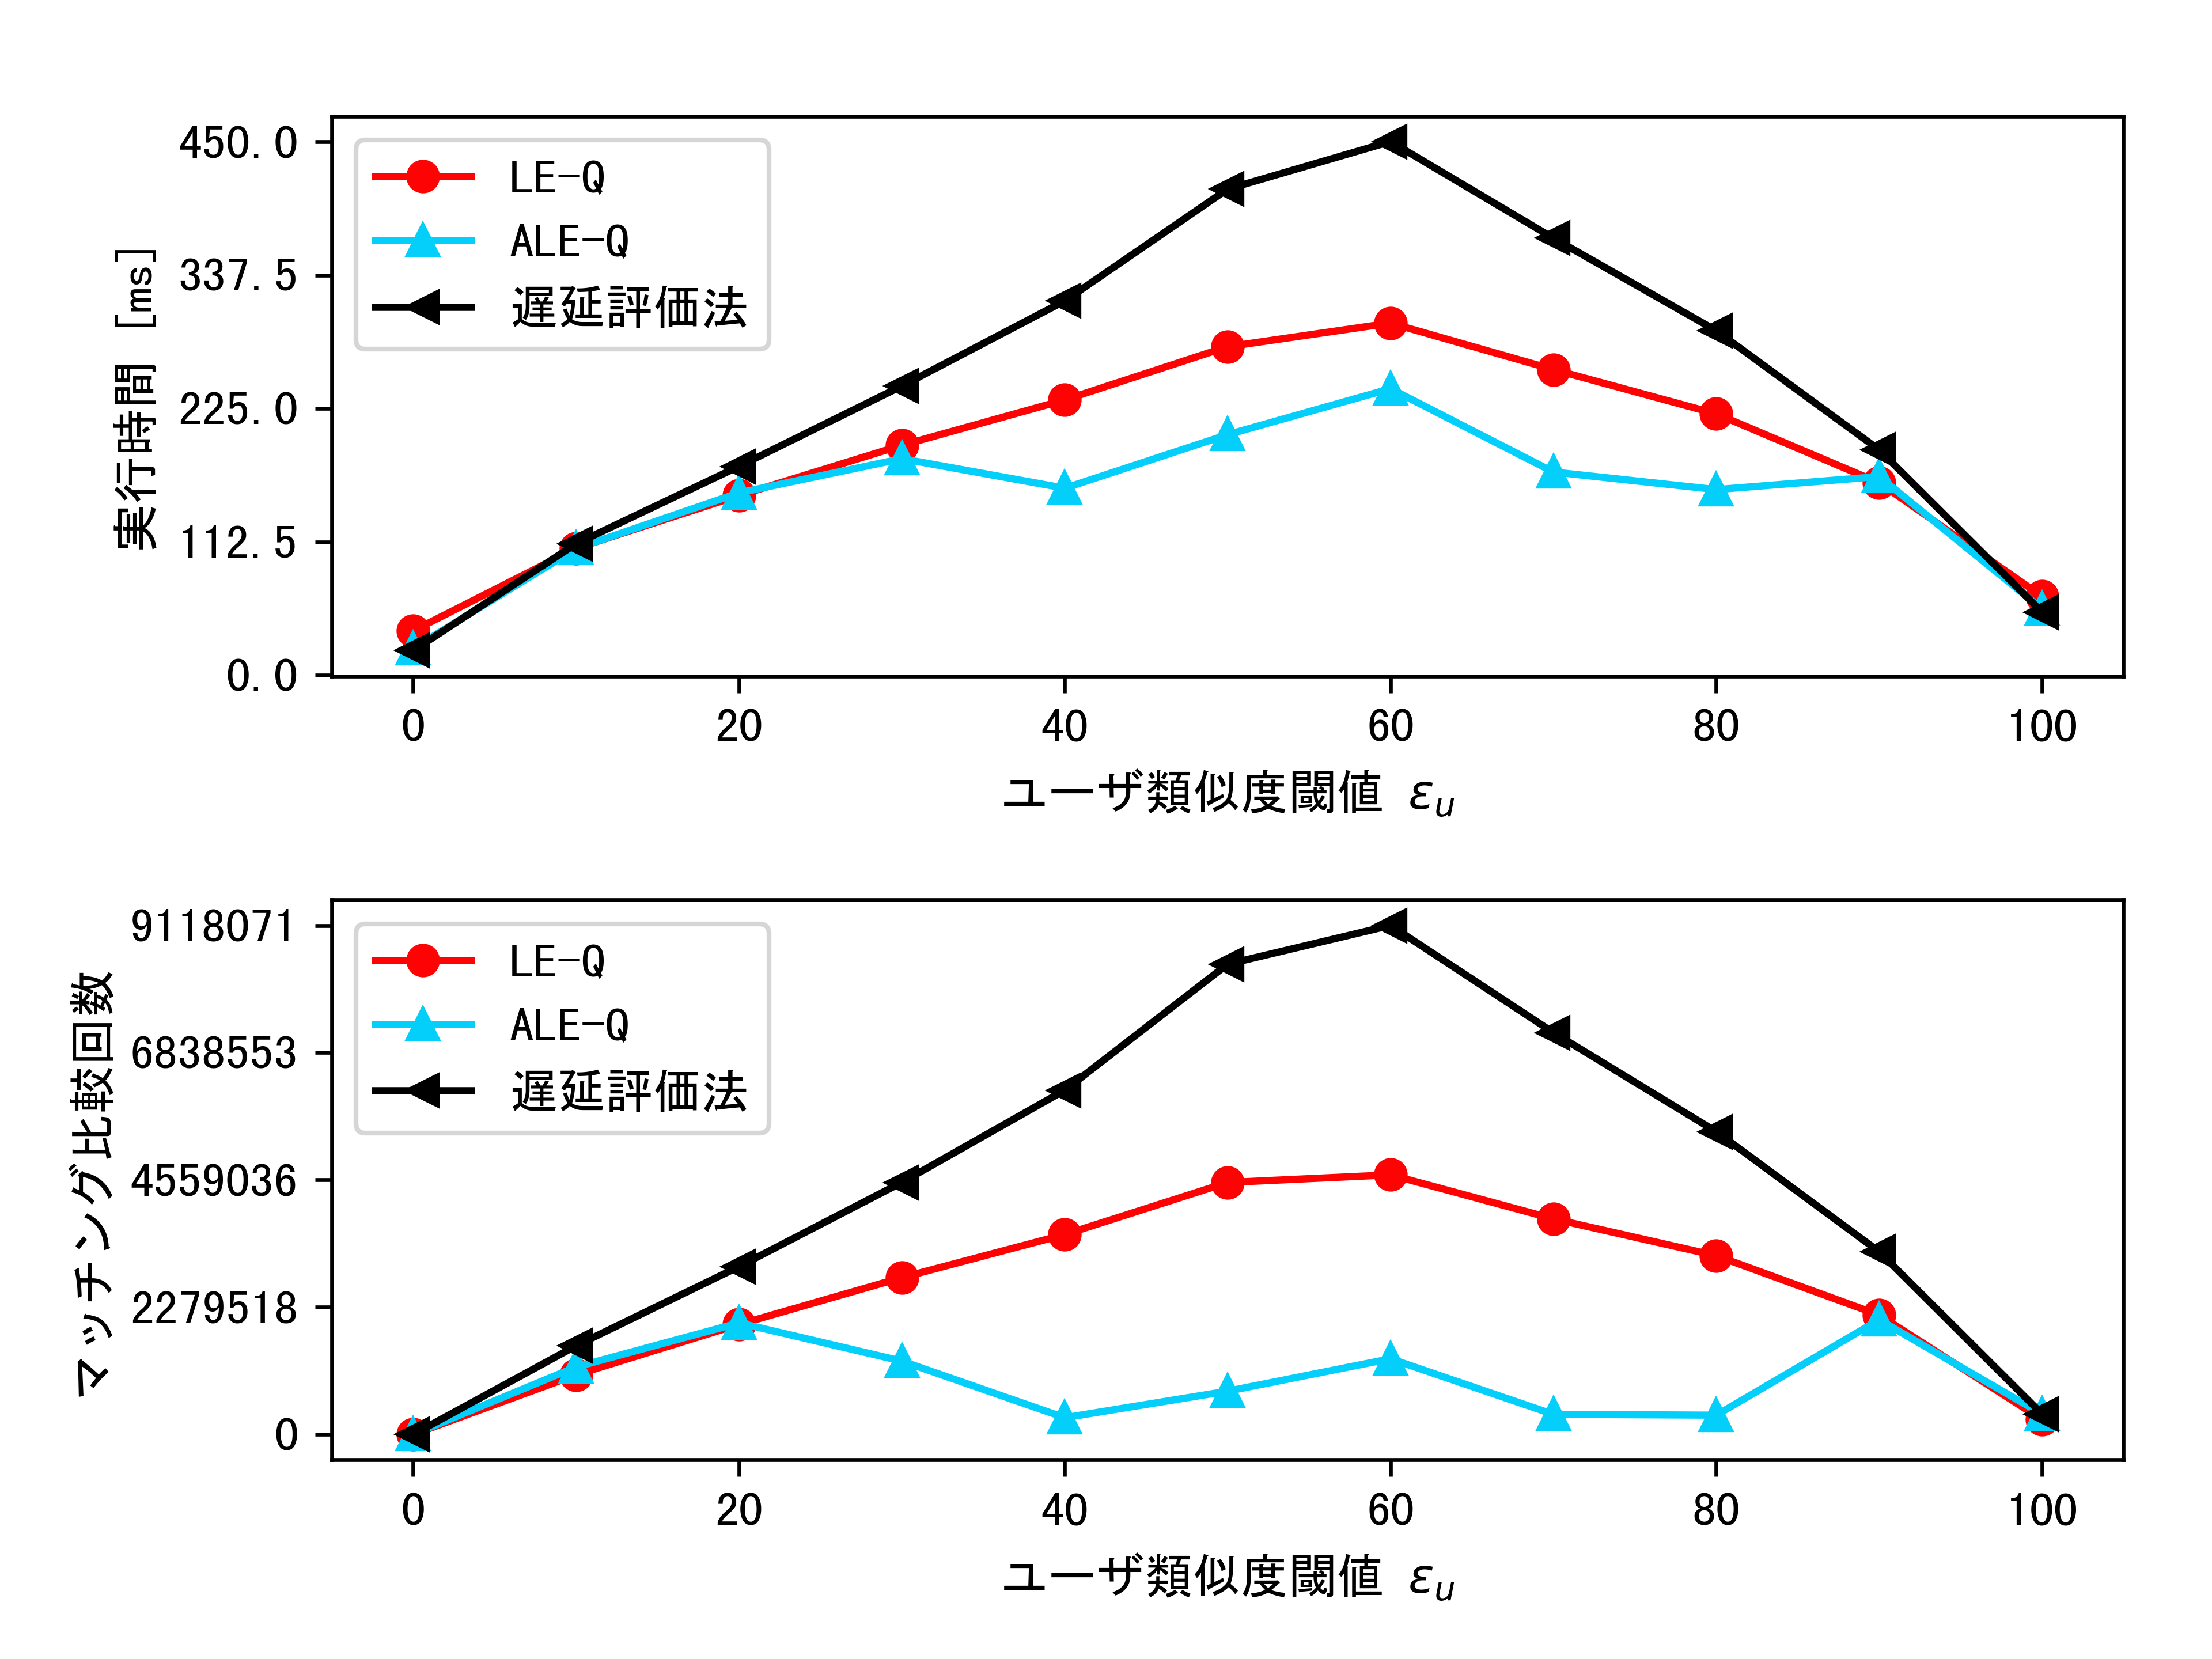
\includegraphics[width=8.3cm]{eimg/exp3_9.png}
    \caption{ALE-Qの性能比較(人工データセット($p=0.9$))}
    \label{fig:exp3_9}
\end{figure}

%よって,ALE-QをCTS問題の最も効率的なアルゴリズムであると結論付ける.